%% Mémoire de Master CyberVault — édition canonique en un seul fichier
%% Compilation : pdflatex -> pdflatex (bibliographie intégrée)
\documentclass[11pt,a4paper,oneside]{report}

\usepackage[utf8]{inputenc}
\usepackage[T1]{fontenc}
\usepackage[english,main=french]{babel}
\usepackage{lmodern}
\usepackage{microtype}
\usepackage{geometry}
\geometry{top=2.5cm,bottom=2.5cm,left=2.7cm,right=2.4cm}
\usepackage{setspace}
\setstretch{1.35}
\usepackage{amsmath,amssymb,amsfonts,amsthm}
\usepackage{booktabs,array,longtable,multirow,tabularx}
\usepackage{graphicx}
\graphicspath{{figures/}}
\usepackage{float}
\usepackage{caption}
\usepackage{subcaption}
\usepackage{enumitem}
\usepackage{xcolor}
\usepackage{url}
\usepackage{hyperref}
\usepackage{cleveref}
\usepackage{algorithm}
\usepackage{algpseudocode}
\usepackage{tikz}
\usetikzlibrary{arrows.meta,positioning,fit,calc,backgrounds,shapes.geometric}
\usepackage{fancyhdr}
\usepackage{titlesec}

\definecolor{cv1}{RGB}{41,98,255}
\definecolor{cv2}{RGB}{0,150,136}
\definecolor{cv3}{RGB}{245,124,0}
\definecolor{cv4}{RGB}{142,36,170}
\definecolor{cv5}{RGB}{198,40,40}
\definecolor{cvg}{RGB}{55,71,79}

\hypersetup{
  colorlinks=true,
  linkcolor=black,
  citecolor=cv1,
  urlcolor=cv1,
  pdfauthor={Oumaima Alfairam},
  pdftitle={CyberVault : détection comportementale hybride et réponse sous contraintes pour les sessions d'accès privilégié}
}
\urlstyle{same}

\theoremstyle{definition}
\newtheorem{definition}{Définition}[chapter]
\newtheorem{assumption}{Hypothèse}[chapter]
\theoremstyle{plain}
\newtheorem{proposition}{Proposition}[chapter]

\titleformat{\chapter}[display]
  {\normalfont\huge\bfseries}{\chaptertitlename\ \thechapter}{15pt}{\Huge}
\titlespacing*{\chapter}{0pt}{-8pt}{28pt}

\pagestyle{fancy}
\fancyhf{}
\fancyhead[L]{\small CyberVault}
\fancyhead[R]{\small\nouppercase{\leftmark}}
\fancyfoot[C]{\thepage}
\renewcommand{\headrulewidth}{0.3pt}
\setlength{\headheight}{14pt}

\begin{document}
\selectlanguage{french}

% ------------------------------------------------------------------
% Pages liminaires
% ------------------------------------------------------------------
\begin{titlepage}
\centering
{\large Université Moulay Ismaïl, Meknès}\\[0.2cm]
{\large Faculté des sciences}\\[0.2cm]
{\large Master Intelligence artificielle et recherche opérationnelle (IARO)}\\[1.5cm]

{\Large\bfseries MÉMOIRE DE MASTER}\\[1.0cm]
\rule{\textwidth}{0.8pt}\\[0.65cm]
{\LARGE\bfseries CyberVault : détection comportementale hybride\\[0.22cm]
et réponse sous contraintes pour les\\[0.22cm]
sessions d'accès privilégié sur JumpServer}\\[0.65cm]
\rule{\textwidth}{0.8pt}\\[1.25cm]

\begin{minipage}{0.88\textwidth}
\begin{tabular}{@{}ll@{}}
\textbf{Auteure :} & Oumaima Alfairam \\[0.25cm]
\textbf{Encadrant :} & Prof. Khalid El Yassini \\
& Équipe de recherche IAOR, Laboratoire IA, UMI \\[0.25cm]
\textbf{Co-encadrante :} & Prof. Kenza Oufaska \\
& Laboratoire LERMA, Université Internationale de Rabat \\[0.25cm]
\textbf{Organisme d'accueil :} & Venthone Luxembourg \\[0.25cm]
\textbf{Période du projet :} & 28 mars 2026 -- 8 juillet 2026 \\
\textbf{Année universitaire :} & 2025--2026
\end{tabular}
\end{minipage}

\vfill
{\small Mémoire présenté en vue de l'obtention du diplôme de Master IARO.}
\end{titlepage}

\pagenumbering{roman}

\chapter*{Déclaration}
\addcontentsline{toc}{chapter}{Déclaration}
Je déclare que ce mémoire rend compte du projet CyberVault tel qu'il a été mis en œuvre et évalué dans le dépôt qui l'accompagne. Les idées externes et les travaux antérieurs sont signalés au moyen de citations. Les affirmations relatives à l'état de l'implémentation et aux performances expérimentales se limitent au code source conservé et aux artefacts de mesure disponibles. Des outils d'assistance au code, de révision linguistique et de structuration du document ont été utilisés sous la responsabilité de l'auteure ; l'ensemble des interprétations techniques, des affirmations expérimentales et de la formulation finale a été vérifié au regard des éléments probants du projet.

\chapter*{Remerciements}
\addcontentsline{toc}{chapter}{Remerciements}
Je remercie le Prof. Khalid El Yassini pour son encadrement et pour m'avoir régulièrement conduite à distinguer, au sein du projet, ce qui relevait d'une contribution scientifique de ce qui procédait de l'intégration logicielle. Je remercie également la Prof. Kenza Oufaska pour nos échanges sur la modélisation multi-objectifs et pour avoir souligné qu'un modèle d'optimisation doit représenter les contraintes opérationnelles, et non uniquement une fonction objectif. Enfin, j'exprime ma gratitude à l'équipe pédagogique du Master IARO ainsi qu'à ma famille pour leur soutien tout au long du projet.

\chapter*{Abstract}
\addcontentsline{toc}{chapter}{Abstract}
Privileged Access Management (PAM) systems mediate and record administrator sessions, yet recording alone does not assess whether behaviour remains acceptable after access has been granted. This thesis presents \textbf{CyberVault}, an operational analytics layer integrated with the open-source JumpServer bastion. The system combines deterministic command and policy rules, per-user User and Entity Behaviour Analytics (UEBA), an Isolation Forest--Random Forest tabular detector, conditional SHAP/LIME explanations, and a constraint-aware response policy. The architecture separates computed evidence from response authority: model scores are fused conservatively, while lock and termination actions remain subject to protected-account and confidence constraints.

The implementation instruments JumpServer command, authentication, and session events, publishes them through asynchronous file, Redis, HTTP, or Kinesis producers, and processes them in a separate Python service. Experiments combine adapted public corpora (CERT Insider Threat, LANL), laboratory PAM telemetry, and a complementary synthetic benchmark. On the 300-event test fold, hybrid fusion achieves an $F_1$ score of $66.23\%$ and recall of $81.97\%$, a clear gain over rules alone ($51.22\%$ F$_1$, $34.43\%$ recall). Technical validations include Docker deployment, JumpServer integration, SSH/RDP sessions, response actions, and an AWS EC2 proof of concept. A bounded multi-objective response comparison completes the evaluation. The thesis contributes an inspectable AI--OR architecture, an implementation-grounded formalisation, and a systematic evidence audit. Limitations and priority perspectives are consolidated in a dedicated section.

\medskip
\noindent\textbf{Keywords:} privileged access management, insider threat, anomaly detection, UEBA, explainable AI, multi-objective optimisation, JumpServer.

\chapter*{Résumé}
\addcontentsline{toc}{chapter}{Résumé}
Les plateformes de gestion des accès privilégiés (PAM) centralisent et enregistrent les sessions d'administration, mais l'enregistrement ne permet pas, à lui seul, d'évaluer si le comportement demeure acceptable au cours d'une session active. Ce mémoire présente \textbf{CyberVault}, une couche analytique opérationnelle intégrée au bastion open source JumpServer. Le système combine des règles déterministes relatives aux commandes et aux politiques, un profilage comportemental UEBA propre à chaque utilisateur, un détecteur tabulaire associant Isolation Forest et Random Forest, des explications conditionnelles SHAP/LIME, ainsi qu'une politique de réponse soumise à des contraintes de sécurité. L'architecture distingue les éléments probants calculés du pouvoir de décision : les scores des modèles sont fusionnés de manière conservatrice, tandis que le verrouillage ou l'interruption d'une session restent soumis à des contraintes relatives aux comptes protégés et au niveau de confiance.

L'implémentation instrumente les commandes, les authentifications et les événements de session de JumpServer, les publie via des producteurs asynchrones (fichier, Redis, HTTP, Kinesis) et les traite dans un service Python dédié. Les expérimentations s'appuient sur des corpus publics adaptés (CERT Insider Threat, LANL), sur la télémétrie d'un laboratoire PAM et sur un benchmark synthétique complémentaire. Pour l'ensemble de test de 300 événements, la fusion hybride atteint un score $F_1$ de $66{,}23\%$ et un rappel de $81{,}97\%$, soit un gain net par rapport aux règles seules ($51{,}22\%$ de F$_1$, $34{,}43\%$ de rappel). Des validations techniques (Docker, intégration JumpServer, sessions SSH/RDP, actions de réponse, POC AWS) et une comparaison bornée de politiques multi-objectifs complètent ce volet. Ce mémoire contribue une architecture IA--RO inspectable, une formalisation ancrée dans l'implémentation et un audit systématique des éléments probants. Les limites et les perspectives prioritaires sont rassemblées dans une section dédiée.

\medskip
\noindent\textbf{Mots-clés :} gestion des accès privilégiés, menace interne, détection d'anomalies, UEBA, IA explicable, optimisation multi-objectifs, JumpServer.

\chapter*{Liste des abréviations}
\addcontentsline{toc}{chapter}{Liste des abréviations}
\begin{longtable}{@{}ll@{}}
ACL & Liste de contrôle d'accès \\
API & Interface de programmation d'application \\
CERT & Jeu de données du Computer Emergency Response Team sur les menaces internes \\
DL & Apprentissage profond \\
FPR & Taux de faux positifs \\
GNN & Réseau de neurones sur graphes \\
IF & Isolation Forest \\
JIT & Accès privilégié juste-à-temps \\
LANL & Jeu de données du Los Alamos National Laboratory \\
LIME & Explications locales interprétables indépendantes du modèle \\
LSTM & Mémoire à long et court terme \\
ML & Apprentissage automatique \\
MOO & Optimisation multi-objectifs \\
PAM & Gestion des accès privilégiés \\
RF & Random Forest \\
SHAP & Explications additives de SHapley \\
SIEM & Gestion des informations et des événements de sécurité \\
SOAR & Orchestration, automatisation et réponse en matière de sécurité \\
SOC & Centre des opérations de sécurité \\
UEBA & Analyse du comportement des utilisateurs et des entités \\
WIP & Travail en cours \\
XAI & Intelligence artificielle explicable \\
\end{longtable}

\tableofcontents
\listoffigures
\listoftables
\clearpage
\pagenumbering{arabic}

% ================================================================

% restore

\chapter{Introduction générale}
\label{chap:intro}

\section{Présentation de l'organisme d'accueil}
\label{sec:intro-venthone}

Venthone, fondée en 2002 et établie à Capellen (Luxembourg), est une société
européenne de consultance et de \emph{payrolling}, avec une présence au
Luxembourg, en France, en Belgique, en Allemagne et au
Portugal~\cite{paperjam2026venthone,venthone2026about,venthone2026home}. Elle
accompagne consultants et clients sur les aspects contractuels, administratifs,
financiers et juridiques des missions, et propose des outils numériques
(\emph{onboarding}, suivi du temps et des dépenses, tableaux de bord). Cette
activité, fondée sur des identités, des rôles et des données sensibles,
fournit le contexte professionnel du stage ; CyberVault demeure toutefois un
travail autonome de recherche appliquée.

\section{Cadre du stage}
\label{sec:intro-stage}

Le stage s'est déroulé du 28 mars au 8 juillet 2026 et a offert le cadre
professionnel pour étudier la surveillance des accès privilégiés,
depuis la formulation du besoin jusqu'à la réalisation d'un prototype fonctionnel.
Le travail a consisté à examiner comment une plateforme de gestion
des accès privilégiés pouvait être complétée par une couche d'analyse
comportementale, puis à formaliser, implémenter et évaluer cette proposition.
La démarche associe étude
bibliographique, spécification, développement logiciel, expérimentation et
analyse des preuves produites.

CyberVault est un prototype de recherche opérationnel construit autour de JumpServer. Les
expérimentations combinent des corpus publics de référence (notamment CERT
Insider Threat et LANL), des traces produites dans un laboratoire PAM
contrôlé, des scénarios synthétiques complémentaires, ainsi que des
validations techniques de bout en bout couvrant le déploiement, l'intégration et la réponse.
Les données utilisées proviennent exclusivement de sources publiques et de
laboratoire. La
validité scientifique de CyberVault repose sur les méthodes, le code
et les artefacts expérimentaux explicitement examinés, dont la portée et les limites sont détaillées au chapitre Discussion.

\section{Besoin métier : surveiller l'usage des privilèges}
\label{sec:intro-motivation}

Les comptes privilégiés concentrent des capacités dont l'abus peut avoir des
conséquences majeures. Un administrateur système, un opérateur cloud, un
propriétaire de base de données, un compte de service ou une identité
d'urgence peut modifier une politique de sécurité, accéder à des informations
sensibles, déployer un logiciel ou interrompre un service. La gestion des
accès privilégiés, ou PAM, réduit cette exposition en encadrant les
habilitations, en protégeant les secrets, en servant d'intermédiaire aux
connexions et en enregistrant les sessions~\cite{ref1,ref2,ref5}. Un bastion
tel que JumpServer relie ainsi une identité authentifiée à un actif et à un
compte cibles tout en conservant des traces d'audit.

Ces contrôles répondent principalement aux questions « qui peut accéder à
quoi ? » et « dans quelles conditions ? ». Ils ne suffisent pas à déterminer
si chaque action demeure légitime une fois la session ouverte. Un accès
valide peut être utilisé par un acteur interne malveillant, détourné après une
compromission ou conduire à une erreur d'administration dangereuse. Le besoin
métier porte donc sur la période qui suit l'authentification : détecter assez
tôt les comportements risqués, fournir des éléments compréhensibles à
l'analyste et recommander une réponse proportionnée.

La difficulté est double. D'une part, certaines opérations correspondent à
des interdits explicites, alors que d'autres ne deviennent suspectes qu'en
fonction d'un profil, d'un horaire, d'une adresse source ou d'une succession
d'accès. L'UEBA et les méthodes d'apprentissage peuvent compléter les règles
pour traiter ce contexte~\cite{ref7,ref24,ref27}. D'autre part, un score élevé
oriente la décision : un faux positif peut mobiliser un
analyste ou interrompre une opération critique. La réponse reste donc
traçable, graduée et soumise à des contraintes, notamment pour les comptes
protégés. Les explications éclairent l'origine d'un signal et soutiennent le
triage ; leur valeur opérationnelle s'apprécie conjointement avec la
gouvernance de la réponse~\cite{ref12,ref13,ref25}.

\section{Problématique et périmètre}
\label{sec:intro-problem}

La problématique consiste à transformer un événement de session privilégiée
en une recommandation de réponse inspectable et compatible avec des exigences
de sûreté. À partir d'informations portant sur l'identité, la session,
l'actif, le compte cible, la source, l'heure et la commande, le système doit
produire des indices complémentaires, préserver leur provenance, expliquer
les sorties lorsque cela est possible, puis choisir une action parmi un
ensemble borné. CyberVault répond à ce problème par un service analytique
adjacent au plan de contrôle PAM, et non par le remplacement de ce dernier.

JumpServer conserve l'authentification, l'autorisation, la médiation des
identifiants, l'enregistrement des sessions et l'application éventuelle des
décisions. CyberVault reçoit certains événements, maintient un état limité par
session et par utilisateur, combine règles, profilage comportemental et
modèles tabulaires, puis journalise une recommandation. Les réponses possibles
sont graduées, de l'absence d'action à l'interruption, avec des mécanismes de
protection destinés à empêcher une mesure irréalisable ou trop risquée.

Le modèle de menace commence après l'authentification d'un accès privilégié.
Il couvre les usages malveillants, compromis ou dangereux qui restent
observables dans la télémétrie PAM. Il exclut les activités contournant
JumpServer, la compromission du bastion ou du service analytique, la
falsification des événements, l'attribution juridique d'une intention et les
actions invisibles au point d'observation. Les modèles séquentiels ou
graphiques expérimentaux ne font pas partie du noyau évalué ; l'optimisation
du niveau de privilège demeure consultative et l'exécution perturbatrice est
désactivée par défaut. Le périmètre correspond donc à un banc d'essai
intégré, non à une défense PAM autonome prête pour la production.

\section{Questions de recherche}
\label{sec:intro-rqs}

La question principale de recherche (\emph{Main Research Question}, MRQ) qui
guide cette étude est la suivante :
\begin{quote}
\emph{Comment un cadre intégré d'intelligence artificielle, d'IA explicable
et de recherche opérationnelle peut-il améliorer la détection en temps réel,
l'explication et l'optimisation de la réponse pour les sessions d'accès
privilégié sur une plateforme PAM open source ?}
\end{quote}

Cette MRQ est décomposée en quatre sous-questions (\emph{Sub-Research
Questions}, SRQ) :
\begin{itemize}[leftmargin=1.5em]
  \item \textbf{SRQ1 (Détection)~:} Un ensemble hybride (règles expertes, UEBA
  comportemental, apprentissage tabulaire et scoreurs de séquence/graphe)
  peut-il détecter les anomalies de comptes privilégiés plus efficacement que
  chaque moteur isolé sur une télémétrie PAM reproductible ?
  \item \textbf{SRQ2 (Explicabilité)~:} Les attributions SHAP et LIME,
  combinées aux justifications textuelles des règles et de l'UEBA,
  peuvent-elles rendre les alertes actionnables pour les analystes SOC
  pendant les sessions en cours ?
  \item \textbf{SRQ3 (Optimisation)~:} Une sélection de réponse
  multi-objectifs peut-elle surpasser les politiques à seuils statiques
  lorsque les contraintes d'interruption et les comptes protégés
  s'appliquent ?
  \item \textbf{SRQ4 (Intégration)~:} Une conception conjointe du pipeline
  produit-elle un gain de détection mesurable par rapport à une utilisation
  séquentielle ou isolée des moteurs ?
\end{itemize}

Les Chapitres~\ref{chap:impl} et~\ref{chap:discussion} traitent les
SRQ1--SRQ4 à partir des preuves du banc d'essai et des mesures du prototype.

\section{Objectifs}
\label{sec:intro-objectives}

Le projet poursuit cinq objectifs. Le premier est de définir l'événement
analysé, les caractéristiques observables, le modèle de menace et les
frontières de confiance. Le deuxième consiste à formaliser un détecteur
hybride dont les signaux déterministes, comportementaux, non supervisés et
supervisés restent séparément inspectables. Le troisième vise à distinguer le
calcul du risque de la décision, en représentant les coûts des réponses et les
contraintes propres aux comptes sensibles. Le quatrième est de construire le
chemin technique reliant l'instrumentation de JumpServer à l'ingestion,
l'enrichissement, la notation, la journalisation et, sous conditions, aux
appels de contrôle. Enfin, le cinquième objectif est d'évaluer le prototype
sans dépasser la force des preuves disponibles, en documentant les menaces sur
la validité, les difficultés de reproductibilité et les travaux nécessaires à
une validation opérationnelle.

\section{Contributions}
\label{sec:intro-contributions}

Le mémoire apporte d'abord une architecture intégrée opérationnelle qui sépare clairement
l'autorité PAM du service analytique et relie l'observation, l'état, les
détecteurs, l'explicabilité, la décision et l'exécution simulée. Il propose
ensuite une formalisation inspectable du chemin décisionnel couvrant la représentation
des événements, les scores des moteurs, leur fusion, les conditions d'explication,
la gradation des actions et les contraintes d'interruption.

La troisième contribution est un prototype fonctionnel intégré à JumpServer et
accompagné d'un audit systématique de son état réel. Cet audit établit les fonctions
effectives, identifie les capacités partielles et distingue les extensions envisagées,
notamment en matière de transport, de persistance, de sécurité de
configuration et d'application des décisions. Le travail fournit également une
évaluation expérimentale structurée en plusieurs volets : adaptation réussie de corpus publics
(CERT, LANL) démontrant la capacité d'ingestion de données standardisées, comparaison des détecteurs et des politiques de réponse sur un
benchmark PAM conservé, validation opérationnelle du pipeline
JumpServer--CyberVault (déploiement Docker, intégration SSH/RDP, POC AWS), et examen de stratégies de décision multi-objectifs.
Ces artefacts soutiennent une comparaison descriptive et une preuve de concept
intégrée. Les conditions nécessaires à une validation opérationnelle complète ainsi que les perspectives prioritaires sont rassemblées dans une section unifiée du chapitre Discussion.

\section{Conduite du projet}
\label{sec:intro-pilotage}

Le projet a été conduit selon une approche Agile légère, de type Kanban,
adaptée à une preuve de concept exploratoire. Les travaux ont été organisés
par lots successifs (instrumentation JumpServer, moteurs de détection,
politique de réponse, interface et validation), avec un suivi simple de
l'avancement plutôt qu'un formalisme Scrum complet. Cette conduite a permis
d'ajuster rapidement les priorités lorsque des hypothèses techniques étaient
infirmées ou lorsque le schéma d'événements était mieux compris. Les détails
de backlog, de risques et de planification ne sont pas reproduits ici : le
mémoire privilégie la contribution scientifique et technique ; quelques
éléments complémentaires figurent en annexe
(Annexe~\ref{chap:app-management}).


\section{Organisation du mémoire}
\label{sec:intro-outline}

Le mémoire suit la structure recommandée par le Guide PFE du Master IARO.
La présente introduction générale situe le contexte, la problématique, les
objectifs, la méthodologie et les contributions. Le
Chapitre~\ref{chap:sota} présente l'état de l'art sur la PAM, la détection
comportementale et l'optimisation de la réponse, puis identifie le gap
scientifique. Le Chapitre~\ref{chap:method} expose la méthodologie proposée :
conception de CyberVault, formalisation des détecteurs, explicabilité et
politique multiobjectif. Le Chapitre~\ref{chap:impl} décrit
l'implémentation, les données, le déploiement et le fonctionnement en temps
réel, ainsi que les protocoles expérimentaux. Le
Chapitre~\ref{chap:discussion} analyse et discute les résultats, les limites
et les perspectives. La conclusion générale synthétise les apports et ouvre
les travaux futurs. Les annexes rassemblent des éléments de reproductibilité,
de gestion et de configuration.

\chapter{État de l'art}
\label{chap:sota}

\section{Périmètre et démarche d'analyse}

La gestion des accès à privilèges (\emph{Privileged Access Management}, PAM) encadre des opérations d'administration dont l'abus peut causer des dommages étendus. Elle ne se limite ni à authentifier un administrateur ni à chiffrer ses mots de passe : elle relie identité, pouvoir, ressource, justification, durée et trace. Elle associe gouvernance des habilitations, maîtrise des secrets, médiation des connexions, moindre privilège et audit du cycle de vie~\cite{ref1,ref2}.

Ce chapitre réunit fondements et travaux connexes, sans répéter les notions ni assimiler des énoncés commerciaux hétérogènes à des résultats expérimentaux. Trois niveaux de preuve sont distingués : les normes et recherches fondent concepts, limites méthodologiques et critères ; les documentations d'éditeurs établissent des capacités déclarées, sans efficacité comparative ; le code et les artefacts rendent une architecture inspectable, sans prouver la qualité de sa détection. Cette hiérarchie évite d'inférer une architecture interne ou une performance à partir d'une fonction annoncée.

L'analyse suit une session privilégiée : identifier le sujet, obtenir le secret, médiatiser la connexion, observer l'activité, qualifier et expliquer le risque, puis sélectionner une réponse. Elle articule plateformes PAM, UEBA, apprentissage automatique, explicabilité et optimisation multiobjectif. Le PAM décide surtout \emph{qui peut exercer un privilège et par quel canal} ; CyberVault étudie \emph{comment réévaluer et traiter le risque pendant cet exercice}.

Cette lecture privilégie les responsabilités et les points de décision plutôt qu'un inventaire de fonctions. Elle permet de comparer des architectures différentes sans supposer que des termes commerciaux identiques recouvrent les mêmes mécanismes, ni que des composants de recherche testés hors ligne satisfont directement les contraintes d'une session en cours.

\section{Architecture fonctionnelle commune d'une plateforme PAM}
\label{sec:domain-architecture}

Malgré des découpages différents, une architecture PAM peut être lue comme sept fonctions liées. Cette grille compare des responsabilités, qu'elles soient regroupées ou distribuées.

\subsection{Identité, gouvernance et autorisation}

Une identité privilégiée peut être humaine --- administrateur, prestataire ou utilisateur d'urgence --- ou non humaine : compte de service, certificat, robot ou jeton d'API. Le privilège dépend du contexte, notamment des élévations indirectes. La couche d'identité rattache le sujet à des rôles, actifs et politiques, et distingue l'utilisateur réel du compte technique partagé sur la cible.

La décision combine ressource, protocole, temps, origine, motif, approbation et durée. Le juste-à-temps réduit la persistance des droits, la séparation des tâches leur concentration, et la révision périodique les habilitations inutiles. Elle doit aussi conserver le lien entre le demandeur, l'approbateur et le compte effectivement employé. Cette explication normative de l'admission --- telle règle autorise tel accès --- ne qualifie toutefois pas l'activité ultérieure. La gouvernance relie rôles, comptes, contrôles et supervision, mais reste centrée sur l'autorisation~\cite{ref1,ref2}.

\subsection{Coffre-fort et maîtrise des secrets}

Le coffre-fort conserve mots de passe, clés, certificats et jetons. Au-delà du chiffrement, il gouverne leur usage, journalise les opérations et peut injecter l'identifiant dans la connexion sans l'exposer à l'opérateur. Il réduit ainsi copie, réutilisation et divulgation, mais constitue lui-même un actif critique à protéger et sauvegarder.

La rotation renouvelle un secret à échéance, après usage ou événement, réduisant sa fenêtre d'exploitation. Lorsque l'architecture le permet, elle réconcilie la valeur conservée avec celle configurée sur la cible. Elle doit respecter les dépendances, car changer sans coordination un mot de passe de service peut interrompre une application. Surtout, le coffre ne sécurise pas une session déjà autorisée : initié, terminal compromis, détournement ou erreur peuvent agir sans révéler le secret. Les offres PAM associent donc identifiants et sessions~\cite{ref16,ref17,ref18}.

\subsection{Médiation, bastion et contrôle du chemin d'accès}

Le bastion est le point de passage entre opérateur et actifs. Il authentifie le sujet, applique la politique, choisit le compte cible, relaie le protocole et rattache l'activité au contexte. Cette médiation attribue l'usage d'un compte partagé et limite la connectivité directe vers les réseaux sensibles.

Sans remplacer segmentation, pare-feu ou sécurité du poste, ce point de contrôle permet d'évaluer l'exercice du privilège. Selon la logique Zero Trust, ni position réseau ni admission passée ne créent de confiance durable : sujet, ressource et contexte peuvent être réévalués~\cite{ref22,ref47}. Le bastion devient ainsi une frontière d'observation pendant la session.

\subsection{Cycle de session et observation en direct}

Une session suit demande, approbation éventuelle, ouverture, activité, suspension ou terminaison, puis clôture. Selon le protocole, la supervision recueille source, actif, compte, durée, commandes, transferts et contrôles. L'enregistrement sert l'audit a posteriori ; le direct permet d'intervenir avant l'événement suivant. Une archive fidèle peut donc arriver trop tard pour le confinement.

Le traitement en ligne enchaîne événement, enrichissement contextuel, caractéristiques, règles et modèles, score, explication, décision, action et journalisation. La faible latence ne suffit pas : l'observation doit précéder l'effet irréversible et l'action rester sûre. La mesure doit donc séparer temps de collecte, d'inférence, d'explication et d'exécution. Les protocoles graphiques ou chiffrés exposent parfois moins de sémantique qu'une commande textuelle ; l'unité observée --- paquet, événement de contrôle, commande ou session --- doit être précisée.

\subsection{Audit, preuve et redevabilité}

La piste d'audit relie identité, politique, compte technique, cible, événements et interventions. Elle exige intégrité, horodatage, conservation et interrogation. Avec l'apprentissage automatique, elle conserve aussi version du modèle, caractéristiques pertinentes, seuil, raisons et politique de réponse. Cette continuité permet de reproduire la décision et d'expliquer pourquoi deux événements proches ont reçu des traitements différents.

L'audit doit respecter finalités, conservation et droits, et protéger des traces susceptibles de contenir des secrets. Une explication technique n'attribue pas juridiquement une intention : elle rend la décision inspectable, sans transformer un score en preuve de malveillance.

\subsection{Réponse et orchestration}

La réponse traduit le risque en mesure opérable : journaliser, alerter, demander une validation, surveiller davantage, suspendre ou terminer la session, puis éventuellement enquêter ou effectuer une rotation. Ces actions ont des coûts différents : terminer peut arrêter une attaque ou interrompre une restauration ; alerter préserve la continuité mais laisse agir.

L'orchestration formalise les playbooks~\cite{ref15,ref41}, sans toujours exposer le compromis entre sécurité, perturbation et fatigue d'alerte. Les contraintes priment : comptes de secours, opérations vitales ou environnements fragiles peuvent interdire l'arrêt automatique. La réponse doit être gouvernée, traçable et, si possible, réversible.

\section{Modèle de menace à la frontière PAM}
\label{sec:domain-threat}

Les objets protégés sont sessions, actifs, secrets et piste d'audit. Le socle de confiance comprend plateforme PAM, plan de contrôle, service d'analyse, modèles, politiques et canal de réponse. L'analyse vise l'abus d'un initié habilité, le contexte privilégié compromis et l'erreur grave. Cette typologie ne suppose pas que l'intention soit observable : des manifestations proches peuvent relever d'une malveillance, d'un vol d'identifiant ou d'une faute~\cite{ref6}. Le système estime donc un risque opérationnel, non une culpabilité.

Les signaux incluent heure inhabituelle, nouvelle source, cible rare, cadence anormale, déplacement latéral ou commande interdite. Isolés, ils restent ambigus : une intervention nocturne peut être une astreinte. Il faut combiner règles, historique et modèles sans confondre rareté et attaque.

Une connexion contournant le bastion échappe à l'observation ; un plan de contrôle compromis peut falsifier politiques ou traces ; un contenu inaccessible ne peut être analysé. Aucun modèle ne détecte toute attaque, surtout si elle imite une opération habituelle, et la gouvernance peut interdire l'automatisation malgré un risque élevé. Ces exclusions définissent les conditions de validité des décisions.

\section{Fondements analytiques : de l'écart à la réponse}
\label{sec:domain-foundations}

\subsection{UEBA et références comportementales}

L'UEBA (\emph{User and Entity Behaviour Analytics}) construit une référence d'utilisateurs, comptes, sources, actifs ou sessions, puis mesure les écarts. Elle complète l'authentification lorsqu'un identifiant valide apparaît dans un contexte inhabituel~\cite{ref27}. Fréquences, statistiques robustes, valeurs connues et fenêtres temporelles produisent en PAM des signaux lisibles comme « nouvelle source » ou « cible rare ».

Démarrage à froid, dérive et empoisonnement fragilisent toutefois la référence. La première phase manque d'historique ; la seconde déplace progressivement la norme légitime ; le troisième mécanisme tente d'y faire entrer une activité hostile. Rareté des attaques, déséquilibre, qualité des données et faux positifs rendent l'exactitude insuffisante~\cite{ref7,ref24,ref32,ref40}. L'évaluation doit publier précision, rappel, $F_1$, taux de faux positifs et latence, avec partitions temporelles et entités séparées pour éviter les fuites.

\subsection{Apprentissage classique, séquentiel et graphique}

Isolation Forest isole récursivement les observations, des chemins courts signalant les points atypiques~\cite{ref8}. LOF compare la densité locale aux voisinages~\cite{ref19}, tandis que l'OCSVM estime le support des données normales~\cite{ref20}. Utiles avec peu d'attaques étiquetées, leurs scores ne sont pas des probabilités ; mise à l'échelle, contamination, voisinage, noyau et seuil modifient fortement le résultat. Random Forest apprend une discrimination supervisée et des interactions non linéaires~\cite{ref30}, mais reproduit les biais des labels et ignore potentiellement les attaques inédites.

Les ensembles agrègent des détecteurs aux erreurs différentes~\cite{ref48}. Leur gain exige de publier caractéristiques, partitions, hyperparamètres, calibration et fusion ; une faible amélioration moyenne ne compense pas des faux positifs déclenchant des interruptions.

Les LSTM représentent les activités ordonnées et sont étudiés pour les menaces internes~\cite{ref10,ref31,ref44}; les Transformers relient les positions par attention~\cite{ref36}; les réseaux graphiques modélisent entités et accès, donc relations inhabituelles et déplacement latéral~\cite{ref23}. Sans présumer leur supériorité, leur transfert exige données suffisantes, fenêtres ou graphe définis, gestion des nouveaux nœuds, étalonnage, artefacts, budget de latence et comparaison appariée aux modèles tabulaires.

La littérature sur les menaces internes agrège souvent authentifications, fichiers, courriels, navigation et périphériques sur de longues périodes. Diversité des scénarios, labels incertains et corpus isolés limitent la généralisation~\cite{ref6,ref7,ref24,ref32,ref40}. Le jeu synthétique CERT facilite la reproductibilité~\cite{ref43}, mais ne reproduit pas nécessairement les événements d'un bastion. Une performance sur CERT ne démontre donc ni latence en ligne, ni reconnaissance d'une commande dangereuse, ni sûreté de la réponse.

La frontière PAM change l'unité de décision : l'étude rétrospective classe après plusieurs jours, le contrôle de session parfois entre deux commandes. Une fenêtre courte accélère mais appauvrit le contexte ; une longue retarde et peut mélanger plusieurs objectifs administratifs. Le protocole doit distinguer événement, séquence, session et entité, préserver la chronologie et empêcher les fuites d'historique. Les familles doivent être comparées sur les mêmes partitions et le même contexte ; sinon, l'avantage apparent d'un modèle profond peut venir de données supplémentaires plutôt que de son architecture.

\subsection{Explicabilité et limites de l'interprétation}

Une explication justifie un score dans une représentation, sans prouver causalité, correction ou intention. SHAP attribue des contributions inspirées de Shapley~\cite{ref12}; LIME ajuste un substitut local~\cite{ref13}. Fond de référence, perturbations et corrélations influencent les résultats ; fidélité, stabilité, robustesse et utilité doivent être évaluées pour l'usage visé~\cite{ref25}.

En ligne, l'explication peut être réservée aux scores dépassant un seuil afin de maîtriser la latence. Les raisons déterministes et UEBA restent nommées, toute attribution absente est signalée, et modèle comme explicateur sont versionnés. Une explication utile au triage privilégie les éléments contrôlables --- nouvelle cible, horaire, origine ou motif de commande --- plutôt que des dimensions latentes invérifiables. Son utilité se mesure aussi par la capacité de l'opérateur à confirmer ou contester la raison.

\subsection{Optimisation multiobjectif de la réponse}

La sélection d'une action confronte au moins trois objectifs : réduire le risque résiduel, limiter la perturbation et maîtriser la fatigue d'alerte. Pour un événement $e$ et l'ensemble des actions admissibles $\mathcal{A}_{\mathrm{feas}}(e)$, une scalarisation simple s'écrit :
\begin{equation}
 a^*(e)\in\arg\min_{a\in\mathcal{A}_{\mathrm{feas}}(e)}
 \left[\alpha f_{\mathrm{sec}}(a,e)+\beta f_{\mathrm{dis}}(a,e)+\gamma f_{\mathrm{fat}}(a,e)\right].
\end{equation}
Les poids expriment une politique et non une vérité universelle ; cette forme ne calcule pas le front de Pareto complet~\cite{ref39}. Les interdictions d'interrompre un compte protégé ou les exigences minimales de confiance appartiennent à l'ensemble admissible plutôt qu'à une pénalité que le score pourrait compenser. Les travaux sur les défenses, les plans d'incident et leur coût confirment la pertinence d'une décision tenant conjointement compte des conséquences techniques, financières et opérationnelles~\cite{ref33,ref38}.

Une MOO exploitable restitue candidats, coûts, poids, actions éliminées par contrainte et motif de sélection, avec une politique de repli si les données manquent. Les interdictions absolues doivent rester distinctes des préférences pondérées, afin qu'un gain de sécurité estimé ne compense pas une opération interdite. Son bénéfice exige une comparaison aux seuils ou playbooks fixes, notamment lorsqu'une contrainte change effectivement l'action.

L'optimiseur ne corrige ni score mal calibré, ni explication instable, ni coût arbitraire. La conception sépare donc risque, raisons, confiance, contraintes et préférences. La gouvernance peut alors modifier les coûts ou l'admissibilité sans réentraîner le détecteur, et l'évaluation procéder par ablation : règles, UEBA, modèles, fusion, puis réponse.

L'orchestration prend souvent une alerte qualifiée en entrée~\cite{ref15,ref41}, tandis que la recherche multiobjectif traite des défenses ou plans plus longs qu'une commande~\cite{ref33,ref38}. Dans une session PAM, les actions sont moins nombreuses, mais temps et perturbation sont immédiats. Il faut donc démontrer que la réponse est non seulement optimale formellement, mais autorisée, rapide, journalisée et compréhensible.

\section{Plateformes PAM de référence}
\label{sec:domain-products}

\subsection{CyberArk}

CyberArk présente une offre intégrée de protection et de gestion des accès privilégiés~\cite{ref16}, avec coffre, identifiants et contrôle générique des accès ou sessions. Elle constitue à ce titre une référence commerciale pour situer les responsabilités fonctionnelles d'une chaîne PAM. La documentation disponible établit la réunion de la gouvernance, des secrets et des sessions ; elle retient toutefois un niveau de présentation général, sans détailler corpus, caractéristiques, modèles, seuils, fidélité des explications et performances par événement nécessaires à une comparaison méthodologique reproductible avec le pipeline étudié.

\subsection{Delinea Secret Server}

Delinea décrit Secret Server comme une solution PAM centrée sur les secrets~\cite{ref18}. Sont donc retenus le coffre et le contrôle du cycle d'usage des identifiants, ainsi que leur insertion générale dans des politiques d'entreprise. La documentation disponible retient ces responsabilités fonctionnelles, sans détailler connecteurs, algorithmes, modes de déploiement ni évaluation appariée de l'explicabilité en session au niveau de granularité requis pour une comparaison méthodologique homogène.

\subsection{BeyondTrust Privileged Remote Access}

Privileged Remote Access de BeyondTrust est centré sur l'accès distant privilégié~\cite{ref17}. Il fournit donc un point de comparaison pour la médiation : la connexion administrative passe par un contrôle attribué plutôt que par un accès direct. La documentation disponible permet de retenir le contrôle générique des accès et sessions ; l'analyse comparative retient toutefois les éléments documentés concernant l'emplacement de la décision et les preuves publiées, sans extrapoler sur des fonctionnalités d'apprentissage, attributions locales ou fonctions de coût non précisées.

\subsection{JumpServer}

JumpServer fournit une plateforme PAM et un bastion open source~\cite{ref5}. Il centralise et médiatise les accès, associe sessions, identités et actifs, puis produit une télémétrie exploitable par un composant d'analyse. Il constitue ainsi une frontière d'intégration concrète entre plan de contrôle et moteur expérimental. Son ouverture favorise inspection, adaptation et reproductibilité architecturale, sans résoudre nativement la question étudiée ni garantir une sécurité supérieure à une offre commerciale.

JumpServer reste responsable du plan PAM --- identité, autorisation, médiation et session --- tandis que CyberVault construit les signaux, estime et explique le risque, puis propose une réponse gouvernée. Une indisponibilité analytique ne doit pas modifier implicitement la politique d'accès ; toute action perturbatrice passe par une interface autorisée et auditée.

\section{Comparaison prudente des plateformes}

Le tableau~\ref{tab:domain-pam-comparison} synthétise uniquement ce que les sources de référence permettent de défendre. « Non établi » signifie que la citation utilisée ici ne publie pas l'information avec une précision suffisante ; cela ne signifie pas que la fonction est absente. De même, la colonne analytique décrit un positionnement documentaire général et non une mesure comparative. Les quatre plateformes ne sont donc pas classées par performance : elles servent à situer le coffre, la médiation, l'ouverture et la disponibilité de preuves selon un vocabulaire commun.

\begin{table}[htbp]
\centering
\caption{Comparaison fonctionnelle prudente de plateformes PAM de référence.}
\label{tab:domain-pam-comparison}
\scriptsize
\begin{tabular}{@{}p{1.75cm}p{2.25cm}p{1.65cm}p{1.8cm}p{1.75cm}p{1.65cm}p{1.8cm}p{2.05cm}@{}}
\toprule
\textbf{Plateforme} & \textbf{Architecture / déploiement} & \textbf{Coffre} & \textbf{Session} & \textbf{Analytics} & \textbf{Explicabilité publiée} & \textbf{Ouverture / intégration} & \textbf{Limites de la comparaison} \\
\midrule
CyberArk~\cite{ref16}
& Suite PAM commerciale ; détail de déploiement non comparé & Fonction PAM de secrets retenue & Contrôle PAM retenu à un niveau générique & Capacités précises non évaluées ici & Protocole XAI reproductible non établi & Produit commercial ; interfaces précises hors preuve citée & Documentation fournisseur, sans banc d'essai commun \\
Delinea Secret Server~\cite{ref18}
& Solution commerciale centrée sur Secret Server ; options précises non établies & Fonction centrale documentée & Contrôle associé au PAM, sans granularité comparative & Méthodes et résultats non établis & Protocole XAI reproductible non établi & Intégration générique attendue d'un PAM ; détails non affirmés & Source insuffisante pour comparer modèles et seuils \\
BeyondTrust PRA~\cite{ref17}
& Solution commerciale orientée accès distant privilégié & Hors du point principal établi par la citation & Médiation et contrôle d'accès distant & Méthodes et résultats non établis & Protocole XAI reproductible non établi & Interfaces précises hors preuve citée & Périmètre produit différent d'une suite évaluée de bout en bout \\
JumpServer~\cite{ref5}
& Plateforme PAM / bastion open source, déployable et inspectable & Capacité exacte non détaillée dans la comparaison & Frontière de médiation et de télémétrie & Détection comportementale avancée non présumée & Pas de protocole XAI établi par la citation & Code ouvert, favorable à l'intégration expérimentale & Inspectabilité sans preuve automatique d'efficacité \\
\bottomrule
\end{tabular}
\end{table}

Les offres commerciales reposent sur des données, modèles et protocoles internes dont la publication scientifique reste limitée, ce qui restreint ici les possibilités de reproduction méthodologique. Inversement, l'ouverture de JumpServer ne présume pas d'une supériorité intrinsèque : elle facilite une instrumentation contrôlée, dont l'efficacité dépend toujours de la configuration, du déploiement et de l'évaluation.

\section{Comparaison transversale des familles de travaux}
\label{sec:domain-transversal}

Les produits ne représentent qu'une couche de l'état de l'art. Le tableau~\ref{tab:domain-transversal} compare les familles selon les données, le point de décision, l'explication, la réponse, la reproductibilité et la difficulté de transfert vers une session en direct. Il ne classe pas des performances obtenues sur des corpus incompatibles.

\begin{table}[htbp]
\centering
\caption{Comparaison transversale des familles de travaux au regard de la PAM en direct.}
\label{tab:domain-transversal}
\scriptsize
\begin{tabular}{@{}p{2.25cm}p{2.25cm}p{1.75cm}p{1.75cm}p{1.65cm}p{1.7cm}p{2.05cm}@{}}
\toprule
\textbf{Famille} & \textbf{Données} & \textbf{Décision} & \textbf{Explication} & \textbf{Réponse} & \textbf{Reproductibilité} & \textbf{Limite de transfert PAM} \\
\midrule
Gouvernance / PAM~\cite{ref1,ref2,ref5,ref16,ref17,ref18}
& Identités, droits, secrets, sessions & Admission et contrôle & Règle ou politique & Accès et session & Forte si artefacts ouverts ; variable sinon & Peu de protocoles publiés par événement \\
UEBA / menace interne~\cite{ref6,ref24,ref27,ref32,ref40}
& Historiques multi-sources & Écart d'entité & Signal contextuel & Alerte surtout & Corpus synthétiques disponibles & Fenêtres et granularités différentes \\
Anomalie classique~\cite{ref8,ref19,ref20,ref30,ref48}
& Vecteurs avec ou sans labels & Score ou classe & Selon modèle & Non native & Bonne si protocole complet & Calibration, dérive et faux positifs \\
Séquentiel profond~\cite{ref10,ref31,ref44}
& Activités ordonnées & Motif ou séquence & Partielle & Non native & Exige données et artefacts & Fenêtre, état et latence \\
Graphes~\cite{ref23}
& Nœuds, arêtes et temps & Relation ou voisinage & Partielle & Non native & Dépend de la construction & Dynamique du graphe à définir \\
XAI sécurité~\cite{ref12,ref13,ref25}
& Observation et modèle & Après le score & Fonction principale & Non native & Dépend des hypothèses & Coût et utilité en direct \\
Orchestration / MOO~\cite{ref15,ref33,ref38,ref39,ref41}
& Alertes, coûts, contraintes & Après qualification & Coûts ou playbook & Fonction principale & Bonne si politique publiée & Suppose une alerte en amont \\
\textbf{Périmètre CyberVault}
& Événements PAM et profils & Événement en direct & Raisons et attributions & Action contrainte & Pipeline inspectable & Validation externe encore requise \\
\bottomrule
\end{tabular}
\end{table}

La comparaison révèle une discontinuité fonctionnelle : la PAM porte identité, autorisation et exécution ; l'UEBA et les modèles qualifient l'écart ; la XAI expose des facteurs ; l'orchestration et la MOO choisissent la réponse. Les sources retenues dans ce corpus abordent ces dimensions séparément, sans formaliser conjointement cette chaîne complète pour un événement de bastion avec données, seuils, explications, contraintes et mesures communes. Les historiques agrégés sur plusieurs jours ne se transposent pas directement en interruption sûre par session ou commande.

\section{Gap scientifique et positionnement de CyberVault}
\label{sec:domain-gap}

La littérature fournit les composants éprouvés ; leur composition reproductible à la frontière PAM constitue l'opportunité scientifique adressée par ce travail. Les plateformes contrôlent l'accès et établissent des capacités générales ; l'UEBA qualifie l'écart comportemental ; la XAI rend compte des décisions de modèles ; l'orchestration et la MOO sélectionnent des actions défensives. L'opportunité consiste à formaliser l'enchaînement mesurable de ces fonctions complémentaires dans un contexte de session privilégiée en direct.

L'opportunité étudiée peut être formulée ainsi :
\begin{quote}
\emph{concevoir et évaluer un pipeline PAM ouvert et reproductible qui, sur le chemin des événements de sessions privilégiées, combine des règles de politique nommées, des références d'entités protégées, des modèles tabulaires supervisés et non supervisés, une explication locale conditionnelle et une sélection multiobjectif des actions soumise à des contraintes strictes de sécurité des comptes.}
\end{quote}

Cette formulation reconnaît que des produits associent PAM et analyse, tout en constatant que les équations, corpus, partitions, ablations et contraintes communes demeurent généralement non publiés par les fournisseurs. La contribution ne porte donc pas sur un nouvel algorithme d'anomalie, mais sur l'architecture, la traçabilité et l'évaluation rigoureuse de méthodes établies dans ce contexte particulier.

L'opportunité invite à documenter composants, caractéristiques, fusion et versions ; mesurer rareté, faux positifs et pas seulement exactitude ; évaluer disponibilité, stabilité, fidélité et latence des explications ; comparer la sélection multiobjectif aux seuils ou playbooks lorsque les contraintes changent la décision. LSTM, Transformer et graphe demeurent expérimentaux dans ce contexte, leur apport devant être établi par comparaison appariée.

Par rapport aux plateformes commerciales (CyberArk, Delinea, BeyondTrust), CyberVault se positionne comme une contribution ouverte et inspectable : formalisation du pipeline, artefacts de mesure, mode simulation par défaut et séparation explicite entre score, explication et autorité d'exécution sur JumpServer. Face à JumpServer seul, qui enregistre et contrôle sans fusion comportementale multi-moteur publiée, CyberVault apporte la détection hybride, l'explicabilité conditionnelle et une politique de réponse sous contraintes. Cette approche ouverte favorise la reproductibilité et l'adaptation à différents contextes opérationnels.

\section{Synthèse et transition}

Une plateforme PAM gouverne l'identité, protège et renouvelle les secrets, médie la connexion, suit la session, conserve la preuve et exécute les réponses autorisées. Elle fournit contexte et intervention ; l'analyse comportementale en session vient enrichir cette gouvernance. L'état de l'art apporte séparément UEBA, détecteurs, explications et décision multiobjectif ; leur intégration reproductible en session avec interfaces, granularités et protocole communs constitue l'opportunité scientifique de ce travail.

CyberVault se positionne en complémentarité avec JumpServer. Il exploite le flux de session déjà associé à une identité, un compte et un actif, le transforme en risque explicable, puis propose une réponse soumise aux contraintes PAM. JumpServer demeure l'autorité d'accès et d'exécution ; CyberVault apporte une couche analytique et décisionnelle auditable. Cette distinction fonde la contribution originale du projet et oriente la méthodologie du chapitre suivant.

\chapter{Méthodologie proposée}
\label{chap:method}

\section{Finalité, exigences et frontière du système}

CyberVault constitue une couche d'analyse et de réponse complémentaire à
JumpServer. Le système observe les événements produits pendant l'usage d'un
accès privilégié, extrait des indices de risque, produit une décision
explicable et, lorsque la politique l'autorise, peut demander une mesure de
contrôle sur la session concernée. L'architecture préserve la séparation des
responsabilités : l'authentification, l'autorisation initiale, la médiation des
protocoles, l'ouverture des connexions et l'enregistrement des sessions
demeurent sous la responsabilité de JumpServer.

Cette séparation impose cinq exigences : une intégration non intrusive qui ne
bloque pas le PAM en cas d'indisponibilité ; une décision traçable reliant
événement, contexte, moteurs disponibles, motifs, risque, confiance et action ;
une dégradation explicite, jamais assimilée à un événement normal ; des effets
perturbateurs soumis aux comptes protégés, à une confiance minimale et à un
mode de simulation sûr par défaut ; enfin, une distinction entre noyau attesté,
extensions conditionnelles et recommandations sans effet direct.

La frontière d'observation est précise. CyberVault consomme des événements
structurés relatifs aux commandes, aux décisions d'ACL, aux connexions et au
cycle de vie des sessions. Le système exploite l'utilisateur, l'actif, le compte
cible, l'adresse source, l'horodatage et la charge utile selon leur disponibilité.
Cette observation se concentre sur les comportements post-authentification au
niveau applicatif ; la qualité de la décision dépend de la fidélité, de l'ordre
et de la complétude des événements transmis par JumpServer.

\subsection{Exigences fonctionnelles}

Le contrat cible exige une enveloppe versionnée, une validation du schéma et
la préservation de la référence à l'observation. Le service construit un
contexte borné depuis l'état de session et le profil de l'entité, puis
appelle les évaluateurs disponibles. Chacun retourne un statut, des motifs et
un score explicite ; l'orchestrateur fusionne ces résultats et sélectionne une
réponse admissible. Le prototype implémente le flux principal ; la validation
formelle du schéma JSON avant enrichissement et la journalisation préalable à
l'effet constituent des axes de durcissement prévus pour une version
industrielle.

Le système permet à l'analyste de consulter le contexte, les motifs, les
statuts des moteurs et la réponse retenue. L'administrateur peut configurer
les transports, les seuils, les comptes protégés, le mode de simulation et les
canaux d'alerte, puis éprouver cette configuration de manière contrôlée. Le
rejeu réutilise le même contrat d'analyse en marquant l'origine historique de
l'événement. Lorsque les préconditions sont réunies, le système joint une
explication locale, notifie les destinataires, peut demander le verrouillage
ou l'arrêt d'une session et calcule une recommandation de privilège. Ces
fonctions étendent le noyau de manière conditionnelle ou consultative selon
leur nature.

\subsection{Exigences non fonctionnelles}

La conception doit être modulaire et testable : un évaluateur peut être
remplacé ou désactivé sans modifier l'ingestion ni la politique d'effet, et les
dépendances externes restent derrière des interfaces. L'état comportemental
survit à une reprise tout en restant distinct de l'événement courant. La
simulation produit une trace comparable au mode réel sans appeler le système
de référence.

La traçabilité exige de relier chaque dossier à la version du schéma, de la
politique et des adaptateurs effectivement mobilisés. Les entrées doivent être
validées avant leur utilisation, les effets externes doivent être idempotents
autant que possible, et chaque échec d'adaptateur, de notification ou d'action
doit être visible dans l'audit. La confidentialité impose de minimiser les
données conservées et d'empêcher qu'une commande sensible soit recopiée sans
contrôle dans une explication ou un export. Enfin, les secrets nécessaires aux
canaux externes et à l'API JumpServer ne font pas partie de l'événement métier
et ne doivent jamais être incorporés aux sorties d'analyse. Disponibilité et sûreté sont volontairement asymétriques : une indisponibilité
de CyberVault préserve l'accès PAM, tandis qu'une incertitude sur l'exécution
privilégie l'audit et la simulation plutôt qu'une action perturbatrice.

\section{Acteurs et cas d'utilisation}
\label{sec:impl-use-cases}

L'opérateur privilégié est une source indirecte : JumpServer transforme ses
actions en événements. L'analyste examine les décisions, l'administrateur règle
l'intégration et la réponse, et l'ingénieur ML prépare les adaptateurs appris.
Les canaux de notification restent secondaires : leur indisponibilité
n'efface pas une décision enregistrée.

\begin{figure}[H]
\centering
\resizebox{0.99\textwidth}{!}{%
\begin{tikzpicture}[
  actor/.style={draw, rounded corners, fill=cvg!8, align=center,
                minimum width=29mm, minimum height=9mm, font=\scriptsize},
  usecase/.style={draw, ellipse, fill=white, align=center,
                  minimum width=34mm, minimum height=10mm,
                  inner sep=2.5pt, font=\scriptsize},
  corecase/.style={draw, ellipse, fill=cv1!9, align=center,
                   minimum width=34mm, minimum height=10mm,
                   inner sep=2.5pt, font=\scriptsize},
  condcase/.style={draw, ellipse, dashed, fill=cv3!8, align=center,
                   minimum width=34mm, minimum height=10mm,
                   inner sep=2.5pt, font=\scriptsize},
  advisory/.style={draw, ellipse, dash dot, fill=cv4!8, align=center,
                   minimum width=36mm, minimum height=10mm,
                   inner sep=2.5pt, font=\scriptsize},
  boundary/.style={draw, rounded corners, thick, inner sep=5mm},
  assoc/.style={thick},
  umlrel/.style={-{Latex[length=1.8mm]}, dashed, thin, align=center},
  indirect/.style={dotted, thick}
]
\node[actor] (operator) at (-5.8,4.8) {Opérateur\\privilégié};
\node[actor] (jumpserver) at (-5.8,2.8) {JumpServer};
\node[actor] (soc) at (-5.8,-0.3) {Analyste\\SOC/PAM};
\node[actor] (admin) at (-5.8,-3.3) {Administrateur\\CyberVault};
\node[actor] (researcher) at (-5.8,-6.1) {Chercheur /\\ingénieur ML};
\node[actor] (channels) at (13.3,-3.0) {Services de\\notification};

\node[usecase] (configure) at (0,4.7) {Configurer et tester\\l'intégration};
\node[corecase] (ingest) at (0,2.8) {Publier / ingérer\\un événement};
\node[corecase] (analyze) at (4.3,2.8) {Analyser l'événement\\en ligne};
\node[usecase] (enrich) at (8.6,4.7) {Enrichir avec\\le contexte};
\node[usecase] (rules) at (8.6,3.2) {Évaluer règles\\et comportement};
\node[condcase] (ml) at (8.6,1.7) {Appeler les adaptateurs\\appris disponibles};
\node[usecase] (fusion) at (4.3,0.9) {Fusionner les\\évaluations};
\node[condcase] (xai) at (8.6,0.1) {Produire une explication\\conditionnelle};
\node[usecase] (response) at (4.3,-0.7) {Sélectionner une\\réponse admissible};
\node[usecase] (log) at (8.6,-1.2) {Journaliser décision\\et résultat};
\node[condcase] (control) at (4.3,-2.3) {Demander verrouillage /\\arrêt};
\node[condcase] (notify) at (8.6,-2.8) {Notifier\\si requis};
\node[usecase] (investigate) at (0,-0.4) {Consulter, investiguer\\et exporter};
\node[usecase] (replay) at (0,-3.0) {Rejouer un journal\\d'événements};
\node[advisory] (privilege) at (4.3,-5.0) {Recommander un niveau\\de privilège};

\node[boundary, fit=(configure)(ingest)(analyze)(enrich)(rules)(ml)
                         (fusion)(xai)(response)(log)(control)(notify)
                         (investigate)(replay)(privilege),
      label={[font=\small\bfseries]above:CyberVault}] (system) {};

\draw[indirect] (operator) -- node[above, sloped, font=\tiny]
  {activité de session} (jumpserver);
\draw[assoc] (jumpserver) -- (ingest);
\draw[assoc] (jumpserver) -- (control);
\draw[assoc] (soc) -- (investigate);
\draw[assoc] (admin) -- (configure);
\draw[assoc] (admin) -- (investigate);
\draw[assoc] (admin) -- (replay);
\draw[assoc] (researcher) -- (replay);
\draw[assoc] (researcher) -- (privilege);
\draw[assoc] (channels) -- (notify);

\draw[umlrel] (ingest) -- node[above, font=\tiny]{\texttt{<<include>>}} (analyze);
\draw[umlrel] (analyze) -- node[above, sloped, font=\tiny]{\texttt{<<include>>}} (enrich);
\draw[umlrel] (analyze) -- node[above, sloped, font=\tiny]{\texttt{<<include>>}} (rules);
\draw[umlrel] (analyze) -- node[left, font=\tiny]{\texttt{<<include>>}} (fusion);
\draw[umlrel] (analyze) -- node[right, font=\tiny]{\texttt{<<include>>}} (response);
\draw[umlrel] (analyze) -- node[above, sloped, font=\tiny]{\texttt{<<include>>}} (log);
\draw[umlrel] (ml) -- node[above, sloped, font=\tiny, align=center]
  {\texttt{<<extend>>}\\adaptateur disponible} (analyze);
\draw[umlrel] (xai) -- node[right, font=\tiny, align=center]
  {\texttt{<<extend>>}\\seuil + préconditions} (ml);
\draw[umlrel] (control) -- node[right, font=\tiny, align=center]
  {\texttt{<<extend>>}\\action autorisée} (response);
\draw[umlrel] (notify) -- node[right, font=\tiny, align=center]
  {\texttt{<<extend>>}\\politique d'alerte} (response);
\draw[umlrel] (replay) -- node[above, sloped, font=\tiny]{\texttt{<<include>>}} (analyze);
\end{tikzpicture}}
\caption{Cas d'utilisation de CyberVault : noyau systématique, extensions
conditionnelles et recommandation consultative.}
\label{fig:impl-use-cases}
\end{figure}

\subsection{Responsabilités des acteurs}

\begin{table}[H]\centering\small
\begin{tabularx}{\textwidth}{p{2.7cm} X X}\toprule
\textbf{Acteur} & \textbf{Interaction attendue} & \textbf{Hors frontière} \\\midrule
Opérateur privilégié & Produit indirectement des commandes, connexions et changements de session. & JumpServer reste le client SSH/RDP et assure l'authentification. \\
JumpServer & Publie les événements structurés et reçoit, sous conditions, une demande de verrouillage ou d'arrêt. & Conserve l'autorité sur l'identité, les ACL, les sessions et l'exécution réelle du contrôle. \\
Analyste SOC/PAM & Consulte le risque, les motifs, le contexte, la décision et les explications disponibles. & Bénéficie d'indices d'aide à la décision pour investiguer les anomalies. \\
Administrateur CyberVault & Configure les transports, seuils, protections, canaux et mode d'exécution. & Applique les contraintes de sûreté définies dans la politique. \\
Chercheur / ingénieur ML & Produit et qualifie les artefacts utilisés par des adaptateurs conditionnels. & Les entraînements s'effectuent hors ligne, l'inférence en ligne. \\
Services de notification & Transportent un message vers les destinataires configurés. & L'accusé technique confirme l'envoi, le traitement reste humain. \\\bottomrule
\end{tabularx}
\caption{Acteurs, interactions et limites fonctionnelles.}
\label{tab:impl-actors}
\end{table}

\subsection{Spécification des cas d'utilisation de niveau utilisateur}

Les opérations d'enrichissement, d'évaluation, de fusion et de journalisation
du diagramme sont des étapes incluses dans UC-01 ; elles ne constituent pas
des objectifs autonomes pour un acteur humain. Les cinq cas ci-dessous
définissent les interactions de niveau utilisateur.

\paragraph{UC-01 --- Analyser un événement privilégié.}
\textbf{Objectif :} produire un risque, des motifs et une réponse à partir
d'une activité JumpServer. \textbf{Préconditions :} le plugin et un transport
pris en charge sont actifs ; la charge est un JSON décodable ; les répertoires
d'état sont accessibles. \textbf{Scénario nominal :} l'événement est ingéré,
enrichi, évalué par les moteurs disponibles, fusionné, puis soumis à la
politique. L'exécuteur tente l'effet autorisé, journalise décision et résultat,
notifie si nécessaire, puis la baseline est mise à jour sous la porte
d'apprentissage. \textbf{Alternatives :} un JSON invalide est rejeté ; un
champ absent reçoit le traitement par défaut ; un modèle sans artefact renvoie
un statut d'indisponibilité ; en \emph{dry-run}, aucun effet JumpServer n'est
produit ; une erreur d'API ou de notification est inscrite ou absorbée selon
le composant. \textbf{Postconditions :} si le traitement atteint
\texttt{ActionExecutor}, une trace contient la décision et le résultat ; la
persistance des états reste une écriture au mieux.

\paragraph{UC-02 --- Investiguer et exporter une décision.}
\textbf{Objectif :} permettre à l'analyste SOC/PAM de comprendre le contexte
d'une alerte. \textbf{Préconditions :} le journal est lisible et le service de
consultation disponible. \textbf{Scénario nominal :} l'analyste filtre les
enregistrements, ouvre le contexte, examine scores, motifs, statuts et
explication éventuelle, puis exporte les éléments utiles.
\textbf{Alternatives :} une explication peut être absente, un moteur
indisponible ou une ligne mal formée ; ces cas doivent être affichés comme
statuts plutôt que masqués. \textbf{Postconditions :} l'analyse est consultée
sans déclencher de nouvel effet automatique.

\paragraph{UC-03 --- Configurer et tester l'intégration.}
\textbf{Objectif :} paramétrer les transports, seuils, protections, canaux et
mode d'exécution. \textbf{Préconditions :} l'administrateur connaît l'URL et
les identifiants nécessaires et conserve initialement le mode simulation.
\textbf{Scénario nominal :} il renseigne la configuration, teste le webhook et
les canaux, vérifie les statuts, puis autorise séparément les fonctions
nécessaires. \textbf{Alternatives :} jeton absent, API JumpServer inaccessible
ou canal de notification défaillant produisent un test négatif ; la surface
HTTP partiellement authentifiée interdit de considérer ce scénario comme une
administration de production durcie. \textbf{Postconditions :} les paramètres
actifs et le résultat du test sont observables, sans passage implicite au mode
réel.

\paragraph{UC-04 --- Rejouer un journal d'événements.}
\textbf{Objectif :} appliquer le même processeur à un corpus historique.
\textbf{Préconditions :} le fichier JSON/JSONL est disponible, les actions sont
neutralisées et l'état de rejeu est isolé. \textbf{Scénario nominal :} les
événements sont marqués comme historiques et traités dans l'ordre par le
pipeline commun. \textbf{Alternatives :} les lignes invalides sont rejetées,
les volumes excessifs doivent être bornés et l'absence d'isolement peut
contaminer profils et compteurs. \textbf{Postconditions :} les décisions de
rejeu sont distinguées des décisions en direct et aucun contrôle réel n'est
autorisé.

\paragraph{UC-05 --- Recommander un niveau de privilège.}
\textbf{Objectif :} fournir une recommandation consultative fondée sur les
coûts et contraintes configurés. \textbf{Préconditions :} le risque, le compte
cible et l'ensemble des niveaux admissibles sont disponibles.
\textbf{Scénario nominal :} le module calcule les six coûts, élimine les
niveaux interdits et sélectionne le minimum ou une demande admissible dans la
tolérance. \textbf{Alternatives :} \texttt{FULL\_ROOT} est exclu lorsque le
risque ou la protection du compte l'impose ; en cas de données incomplètes, la
recommandation doit rester explicitement consultative.
\textbf{Postconditions :} le niveau proposé est joint à l'audit, sans
modification automatique des ACL JumpServer.

\phantomsection\label{tab:impl-use-cases-summary}

\section{Architecture fonctionnelle et niveaux de capacité}

L'architecture adopte une chaîne de responsabilités plutôt qu'un détecteur
monolithique. La couche d'intégration reçoit des événements depuis JumpServer
ou depuis une source de rejeu. La couche de contexte interprète les identifiants
disponibles, applique les valeurs par défaut et consulte les magasins d'état.
La validation formelle contre le schéma reste une cible non reliée au
processeur courant. La couche
d'analyse rassemble les contrôles déterministes et comportementaux, auxquels
s'ajoutent des adaptateurs appris lorsque leurs préconditions sont réunies. La
couche de décision fusionne les évaluations, applique la politique de réponse
et prépare une éventuelle recommandation. Enfin, la couche d'effet écrit
l'audit, notifie et appelle, si cela est permis, l'interface de contrôle de
JumpServer.

Trois catégories organisent les fonctions selon leur rôle dans le système.
Les \textbf{capacités centrales} assurent une analyse complète : ingestion,
contrôle syntaxique, enrichissement, règles, profil comportemental, fusion,
sélection d'une réponse et audit. Elles fonctionnent sans modèle appris et
produisent des motifs lisibles. Les \textbf{capacités conditionnelles}
comprennent les adaptateurs tabulaires, séquentiels ou relationnels,
l'explication locale, la notification et les mesures de verrouillage ou
d'arrêt. Leur activation dépend respectivement d'artefacts compatibles, d'un
seuil et d'une référence explicative, d'un canal configuré ou d'une action
admissible en mode réel. Les \textbf{capacités consultatives} proposent une
orientation sans modifier le système de référence. La recommandation de niveau
de privilège appartient à cette catégorie et peut être reliée à un actionneur
d'ACL gouverné lors d'une évolution future.

Chaque adaptateur conditionnel annonce sa disponibilité, les données acceptées,
un score borné, une confiance documentée, des motifs et un statut d'erreur. Il
préserve la séparation entre analyse et effet. Sa catégorie dépend de son rôle
plutôt que de l'implémentation : la présence d'un artefact compatible active
le signal. Une notification reste conditionnelle, tandis que l'audit appartient
au noyau. Le système combine ainsi un socle déterministe et comportemental avec
des adaptateurs évolutifs, offrant une architecture modulaire et extensible.

\begin{figure}[H]
\centering
\begin{tikzpicture}[
  node distance=7mm and 9mm,
  box/.style={draw, rounded corners, align=center, minimum height=9mm,
              minimum width=28mm, fill=white},
  flow/.style={-{Latex[length=2mm]}, thick},
  optional/.style={-{Latex[length=2mm]}, dashed, thick}
]
\node[box, fill=cv1!10] (source) {JumpServer /\\source de rejeu};
\node[box, right=of source, fill=cv2!10] (ingest) {Adaptateurs\\d'entrée};
\node[box, right=of ingest, fill=cv3!10] (processor) {Orchestrateur\\d'analyse};
\node[box, above right=8mm and 11mm of processor, fill=cv3!10] (core)
  {Règles et profil\\comportemental};
\node[box, below right=8mm and 11mm of processor, fill=cv3!10] (adapters)
  {Adaptateurs appris\\conditionnels};
\node[box, right=25mm of processor, fill=cv4!10] (decision)
  {Seuils + repli\\scalarisé};
\node[box, right=of decision, fill=cv5!10] (executor)
  {Audit et\\exécuteur};
\node[box, above=of executor, fill=cvg!10] (channels)
  {Canaux de\\notification};
\node[box, below=of executor, fill=cvg!10] (jsapi)
  {Contrôle de session\\JumpServer};
\node[box, below=18mm of processor, fill=cvg!10] (state)
  {État contextuel, profils\\et artefacts référencés};

\draw[flow] (source)--(ingest);
\draw[flow] (ingest)--(processor);
\draw[flow] (processor)--(core);
\draw[optional] (processor)--(adapters);
\draw[flow] (core)--(decision);
\draw[optional] (adapters)--(decision);
\draw[flow] (decision)--(executor);
\draw[flow] (processor)--(state);
\draw[optional] (executor)--(channels);
\draw[optional] (executor)--(jsapi);
\end{tikzpicture}
\caption{Topologie conceptuelle des composants et séparation entre noyau,
adaptateurs conditionnels, décision et effets externes.}
\label{fig:impl-components}
\end{figure}

\section{Flux de données de haut niveau}
\label{sec:method-dataflow}

Le flux commence par une enveloppe contenant un type, un horodatage et un
identifiant stable, complétés selon le cas par le contexte et une charge utile.
Le transport vérifie que la charge utile est du JSON exploitable. L'enrichissement
produit les indicateurs nécessaires en intégrant l'état disponible. Le prototype
exploite une validation syntaxique légère permettant un enrichissement rapide ;
la validation formelle contre \path{schemas/security_event.json} peut
renforcer la robustesse dans une version ultérieure.

L'enrichissement relie l'événement au contexte de session et au profil, puis
produit les indicateurs nécessaires. La mise à jour du profil intervient après
la décision et seulement si la porte d'apprentissage l'autorise, afin qu'un
événement risqué ne devienne pas immédiatement une norme.

Les évaluateurs reçoivent le même événement enrichi : les règles expriment des
sévérités explicites, le profil mesure l'écart historique et les adaptateurs
disponibles utilisent leur projection contractuelle. La fusion conserve le
signal le plus sévère plutôt qu'un vote moyen. L'explication accompagne une
évaluation apprise sans modifier le risque ni la décision.

\begin{figure}[H]
\centering
\resizebox{\textwidth}{!}{%
\begin{tikzpicture}[
  font=\small,
  box/.style={draw,rounded corners=2pt,align=center,inner sep=5pt,minimum height=0.9cm},
  arr/.style={-{Latex},thick},
  dasharr/.style={-{Latex},thick,dashed}
]
\node[box,fill=cvg!15,minimum width=2.8cm] (js) {événement\\structuré};
\node[box,fill=cv1!16,minimum width=3.0cm,right=0.55cm of js] (en)
  {contrôle minimal\\et enrichissement};
\node[box,fill=cv2!16,minimum width=2.4cm,above right=0.35cm and 0.65cm of en] (rr)
  {règles};
\node[box,fill=cv2!16,minimum width=2.4cm,right=0.65cm of en] (rb)
  {comportement};
\node[box,fill=cv2!16,minimum width=2.7cm,below right=0.35cm and 0.65cm of en] (rm)
  {adaptateurs appris\\disponibles};
\node[box,fill=cv3!18,minimum width=2.5cm,right=0.85cm of rb] (fu)
  {fusion\\risque, confiance};
\node[box,fill=cv4!18,minimum width=2.7cm,above=0.45cm of fu] (xa)
  {explication\\conditionnelle};
\node[box,fill=cv5!16,minimum width=3.0cm,right=0.7cm of fu] (de)
  {seuils + repli\\scalarisé};
\node[box,fill=cvg!12,minimum width=3.0cm,right=0.6cm of de] (ex)
  {effet éventuel ;\\audit du résultat};
\draw[arr] (js)--(en);
\draw[arr] (en)--(rr);
\draw[arr] (en)--(rb);
\draw[dasharr] (en)--(rm);
\draw[arr] (rr)--(fu);
\draw[arr] (rb)--(fu);
\draw[dasharr] (rm)--(fu);
\draw[dasharr] (rm)-|(xa);
\draw[dasharr] (xa)-|(de);
\draw[arr] (fu)--(de);
\draw[arr] (de)--(ex);
\end{tikzpicture}}
\caption{Flux principal : l'explication accompagne l'audit sans influencer le
score, tandis que les adaptateurs appris restent conditionnels.}
\label{fig:method-dataflow}
\end{figure}

La sortie de fusion alimente une politique hybride. Le chemin nominal associe
des intervalles de risque à l'absence d'action, à la journalisation, à l'alerte,
au verrouillage ou à l'arrêt. Si l'action proposée enfreint une contrainte, par
exemple pour un compte protégé ou une confiance insuffisante, le repli
scalarisé compare les actions admissibles selon la sécurité résiduelle, la
perturbation et la fatigue opérationnelle. Cette architecture combine des
\emph{seuils avec repli scalarisé}, permettant des décisions lisibles dans le
cas nominal et une résolution optimisée sous contraintes. L'action finale et
les raisons du repli sont calculées avant l'appel externe ; l'implémentation
journalise le résultat complet après la tentative d'exécution.

\section{Composants logiques et responsabilités de classes}

La conception objet concentre l'orchestration dans \texttt{EventProcessor}.
Celui-ci ne porte pas les règles métier de chaque moteur ; il impose le contrat
du flux, collecte les statuts et construit la décision globale.
\texttt{FeatureStore} fournit le contexte de session et les agrégats
opérationnels, tandis que \texttt{BaselineStore} représente les profils
comportementaux par entité. Leur séparation évite de confondre un historique
technique de traitement et une référence utilisée pour qualifier une anomalie.

Les évaluateurs implémentent une interface commune et retournent un objet
d'évaluation plutôt qu'un nombre isolé. Cet objet contient au minimum le nom et
la version logique du moteur, son état de disponibilité, le risque, la
confiance, les motifs et les avertissements. Le solveur de réponse consomme la
fusion et les contraintes ; il ne lit pas directement les magasins et ne
commande pas lui-même JumpServer. \texttt{ActionExecutor} constitue la frontière
des effets : il délègue le contrôle à \texttt{JumpServerClient}, écrit ensuite
la décision et le résultat, puis sollicite \texttt{AlertNotifier}. Cette
décomposition facilite les essais en simulation et limite les privilèges de
chaque composant.

\begin{figure}[H]
\centering
\resizebox{0.96\textwidth}{!}{%
\begin{tikzpicture}[
  cls/.style={draw,rounded corners,align=left,minimum width=3.4cm,
              minimum height=1.05cm,inner sep=4pt,font=\scriptsize},
  dep/.style={-{Latex[length=1.8mm]},thick},
  optdep/.style={-{Latex[length=1.8mm]},thick,dashed}
]
\node[cls,fill=cv1!12] (processor) at (0,0)
  {\textbf{EventProcessor}\\\texttt{process(event)}\\orchestre une analyse};
\node[cls,fill=cv2!10] (feature) at (-5,-2)
  {\textbf{FeatureStore}\\\texttt{enrich()}\\contexte session/utilisateur};
\node[cls,fill=cv2!10] (baseline) at (-1.7,-2)
  {\textbf{BaselineStore}\\\texttt{load/save()}\\profils par entité};
\node[cls,fill=cv3!10] (detectors) at (1.7,-2)
  {\textbf{Evaluators}\\règles, comportement\\et adaptateurs conditionnels};
\node[cls,fill=cv4!10] (solver) at (5,-2)
  {\textbf{ResponsePolicy}\\\texttt{decide()}\\seuils + repli scalarisé};
\node[cls,fill=cv5!10] (executor) at (1.7,-4.1)
  {\textbf{ActionExecutor}\\audit et effets autorisés};
\node[cls,fill=cvg!10] (client) at (-0.4,-6.1)
  {\textbf{JumpServerClient}\\verrouillage / arrêt};
\node[cls,fill=cvg!10] (notifier) at (3.8,-6.1)
  {\textbf{AlertNotifier}\\canaux et état de remise};
\draw[dep] (processor)--(feature);
\draw[dep] (processor)--(baseline);
\draw[dep] (processor)--(detectors);
\draw[dep] (processor)--(solver);
\draw[dep] (processor)--(executor);
\draw[optdep] (executor)--(client);
\draw[optdep] (executor)--(notifier);
\end{tikzpicture}}
\caption{Responsabilités et dépendances logiques des principales classes.}
\label{fig:impl-classes}
\end{figure}

\subsection{Séquence d'interaction des composants}

Le diagramme de classes décrit les responsabilités statiques ; la
Figure~\ref{fig:impl-sequence} montre immédiatement comment ces composants
coopèrent lors du traitement d'un événement. La frontière asynchrone se situe
autour de Celery et du transport. À partir de l'ingestion, l'analyse devient
ordonnée : décodage, enrichissement, détection, fusion, explication
conditionnelle, décision, exécution et persistance. Les flèches en tirets
représentent des capacités dépendantes d'artefacts ou d'une configuration et
ne doivent pas être lues comme disponibles dans toute installation.

\begin{figure}[H]
\centering
\resizebox{\textwidth}{!}{%
\begin{tikzpicture}[
  lifeline/.style={draw,rounded corners,fill=cv1!8,minimum width=18mm,
                  minimum height=7mm,align=center,font=\scriptsize},
  msg/.style={-{Latex[length=1.7mm]},thick},
  opt/.style={-{Latex[length=1.7mm]},thick,dashed},
  note/.style={font=\tiny,align=center}
]
\node[lifeline] (js) at (0,0) {Hook\\JumpServer};
\node[lifeline] (ce) at (2.2,0) {Celery};
\node[lifeline] (tr) at (4.4,0) {Transport};
\node[lifeline] (pr) at (6.6,0) {Ingestion /\\processeur};
\node[lifeline] (de) at (8.8,0) {Détecteurs};
\node[lifeline] (dx) at (11,0) {Décision /\\XAI};
\node[lifeline] (ex) at (13.2,0) {Exécuteur /\\état};
\foreach \x in {0,2.2,4.4,6.6,8.8,11,13.2}
  \draw[densely dotted] (\x,-0.4)--(\x,-10.7);
\draw[msg] (0,-0.8) -- node[above,note]{enveloppe structurée} (2.2,-0.8);
\draw[msg] (2.2,-1.5) -- node[above,note]{publication au mieux} (4.4,-1.5);
\draw[msg] (4.4,-2.2) -- node[above,note]{fichier / Redis / HTTP} (6.6,-2.2);
\node[note,text=cv5] at (5.5,-2.75) {Kinesis : aucune ingestion};
\draw[msg] (6.6,-3.3) -- node[above,note]{contrôle minimal et enrichissement} (8.8,-3.3);
\draw[msg] (6.6,-4.1) -- node[above,note]{règles puis UEBA} (8.8,-4.1);
\draw[opt] (6.6,-4.9) -- node[above,note]{IF/RF si artefacts} (8.8,-4.9);
\draw[opt] (6.6,-5.7) -- node[above,note]{LSTM/GNN expérimentaux} (8.8,-5.7);
\draw[msg] (8.8,-6.5) -- node[above,note]{scores, confiance, motifs} (6.6,-6.5);
\draw[msg] (6.6,-7.3) -- node[above,note]{fusion ; seuils / repli} (11,-7.3);
\draw[opt] (11,-8.1) -- node[above,note]{XAI de RF seulement} (6.6,-8.1);
\draw[msg] (11,-8.9) -- node[above,note]{action unique} (13.2,-8.9);
\draw[msg] (13.2,-9.7) -- node[above,note]{journal ; notification ; action ou dry-run} (6.6,-9.7);
\draw[msg] (6.6,-10.5) -- node[above,note]{UEBA si \(r\leq.40\) ; persistance / dashboard} (13.2,-10.5);
\end{tikzpicture}}
\caption{Séquence d'interaction des composants pour le traitement d'un
événement. Les modèles, l'XAI, les notifications et les effets JumpServer
sont conditionnels.}
\label{fig:impl-sequence}
\end{figure}

\section{Entrées, sorties et décisions}

Le contrat d'entrée sépare identité technique et contenu analysé. Une entrée
canonique peut être notée
\[
e=(\mathit{id},\mathit{type},t,u,s,v,p,i,q,m),
\]
où \(\mathit{id}\) identifie l'événement, \(t\) est son horodatage, \(u\)
l'utilisateur, \(s\) la session, \(v\) l'actif, \(p\) le compte cible, \(i\)
l'adresse source, \(q\) la charge utile typée et \(m\) les métadonnées. Seuls
l'identifiant, le type et l'horodatage appartiennent au socle commun ; les
autres champs sont requis selon le type. Cette optionalité doit être
représentée explicitement : une valeur absente n'équivaut ni à zéro, ni à une
valeur normale.

L'identifiant permet corrélation et déduplication, le type sélectionne les
validations et les identifiants contextuels relient l'état. La charge utile
reste typée ; les champs inconnus peuvent être conservés, sans influencer
silencieusement la décision. L'enrichissement produit
\(\tilde e=\Gamma(e,H)\), où \(H\) désigne l'état antérieur disponible, sans
fixer les méthodes de calcul traitées dans le chapitre consacré à l'IA.

La sortie principale est un dossier de décision. Il contient la référence à
l'événement, le contexte calculé, la liste des évaluations disponibles, le
risque fusionné, la confiance, les motifs, l'action proposée, les contraintes
appliquées, l'action finale et le résultat d'exécution. Une explication locale
ou une recommandation de privilège peut y être jointe avec son statut
conditionnel ou consultatif. L'audit distingue ainsi quatre faits : une anomalie
a été observée ; une réponse a été choisie ; une tentative d'effet a eu lieu ;
le système externe a confirmé ou refusé cet effet.

La sortie peut être formalisée par
\[
d(e)=\bigl(\mathit{id},\tilde e,\mathcal{Q},r,c,\mathcal{M},
           a^*,\kappa,\xi,\phi,\ell^*\bigr),
\]
où \(\mathcal{Q}\) réunit les évaluations et leurs statuts, \(r\) est le risque
fusionné, \(c\) la confiance de gouvernance, \(\mathcal{M}\) les motifs,
\(a^*\) l'action retenue, \(\kappa\) les contraintes appliquées et \(\xi\)
l'état de l'exécution. L'explication \(\phi\) et le niveau recommandé
\(\ell^*\) sont facultatifs. Le dossier fournit à l'analyste un contexte complet
permettant d'auditer la décision et son exécution.

\section{Modèle conceptuel de décision}
\label{sec:method-formal}

La formalisation de conception distingue les observations, les scores et les
variables de décision. Soit \(\mathcal{E}\) l'ensemble des événements acceptés
et \(\mathcal{A}_{\mathrm{act}}\) l'ensemble fini des réponses :
\[
\mathcal{A}_{\mathrm{act}}=
\{\texttt{NO\_ACTION},\texttt{LOG\_ONLY},\texttt{ALERT\_ANALYST},
\texttt{CREATE\_TICKET},\texttt{LOCK\_SESSION},\texttt{KILL\_SESSION}\}.
\]
Pour un événement \(e\), le risque, la confiance, les motifs et les
contributions explicatives sont des sorties calculées. Ils paramètrent la
politique. La décision active est l'action \(a^*(e)\), unique et appartenant
aux actions admissibles pour cet événement. L'admissibilité dépend du contexte
de gouvernance : compte protégé, confiance minimale, présence d'un identifiant
de session et autorisation du mode réel.

Cette distinction s'écrit avec les variables binaires
\[
y_a(e)\in\{0,1\}\quad(a\in\mathcal{A}_{\mathrm{act}}),
\qquad
\sum_{a\in\mathcal{A}_{\mathrm{act}}}y_a(e)=1,
\]
où \(y_a(e)=1\) signifie que l'action \(a\) est retenue. Le risque \(r\), la
confiance \(c\), les évaluations des règles, du comportement et des
adaptateurs appris, ainsi que les contributions explicatives, restent des
paramètres calculés. La notation \(a^*(e)\) désigne l'unique action sélectionnée.

Le premier niveau de la politique est une application par seuils, lisible par
l'administrateur et stable dans le temps. Le second niveau intervient lorsque
la candidate issue des seuils est interdite. Il sélectionne alors une action
admissible en minimisant un coût scalarisé représentant trois préférences :
réduire le risque résiduel, éviter une perturbation disproportionnée et limiter
la fatigue des analystes. Ces préférences sont des paramètres de politique
validés organisationnellement et versionnés dans l'audit.

Une seconde décision peut proposer un niveau de privilège. Elle obéit également
à une contrainte d'unicité, son résultat restant consultatif : il est joint
au dossier sans provoquer de changement d'ACL. Cette séparation formelle
réserve les effets automatiques aux seules actions dont le chemin de contrôle
est explicitement gouverné.

En notant \(\mathcal{L}\) l'ensemble des niveaux proposés, cette décision
consultative utilise exclusivement
\[
y_\ell(e)\in\{0,1\}\quad(\ell\in\mathcal{L}),
\qquad
\sum_{\ell\in\mathcal{L}}y_\ell(e)=1.
\]
Ainsi, \(y_a\) et \(y_\ell\) sont les seules variables de décision de la
conception. Les fonctions objectives, les coefficients de scalarisation et la
formulation détaillée des contraintes sont volontairement réservés au chapitre
consacré à l'IA et à la recherche opérationnelle. Le présent chapitre fixe
seulement le domaine des choix, leur unicité, leur statut actif ou consultatif
et leur dépendance à des entrées calculées.

\section{Modes de dégradation et garanties minimales}

La dégradation s'organise comme un ensemble d'états explicites assurant la
transparence du système. Lorsqu'un adaptateur appris est absent, incompatible
ou en échec, son statut devient indisponible ; les règles, le profil
comportemental, la fusion des évaluations restantes et l'audit continuent. Le
système signale les phases d'initialisation du profil et les champs facultatifs
manquants, garantissant la traçabilité.

La reprise après perte de l'état contextuel s'effectue en mode dégradé avec un
marquage explicite du démarrage à froid. Les erreurs de persistance distinguent
la décision produite de la garantie de conservation. Les événements mal formés
sont rejetés ou mis en quarantaine avant l'évaluation ; les doublons détectables
sont corrélés à l'identifiant stable pour empêcher la répétition d'un effet.

Les défaillances situées après la décision conservent la trace complète : une
notification indisponible ajoute un état d'échec de remise sans annuler le dossier ;
une API de contrôle inaccessible transforme l'effet en tentative échouée sans
réécrire l'action choisie. Le mode simulation conserve cette séparation, permettant
d'auditer la politique indépendamment de l'infrastructure d'effet.

L'indisponibilité de CyberVault préserve l'authentification, l'autorisation et
la continuité des sessions assurées par JumpServer. Ce choix architectural
privilégie la disponibilité du PAM ; au rétablissement, les lacunes
d'observation restent identifiables, permettant à l'analyste de distinguer
absence de signal et absence de données.

\section{Synthèse de la conception et transition vers les modèles}

La conception établit une frontière claire : JumpServer demeure l'autorité PAM,
tandis que CyberVault valide, contextualise, évalue et trace les événements
post-authentification. Le noyau fonctionne avec des règles et un profil
comportemental ; les modèles et l'explicabilité enrichissent l'analyse comme
adaptateurs conditionnels ; la recommandation de privilège apporte une aide
consultative. Le flux sépare l'observation, le calcul du risque, le choix
d'une action et son effet réel. La réponse s'articule comme une politique à
seuils avec repli scalarisé, soumise à des contraintes explicites.

Cette architecture fournit le cadre nécessaire aux chapitres suivants. La
partie consacrée à l'intelligence artificielle précise comment les adaptateurs
produisent des signaux complémentaires et sous quelles conditions ils sont
interprétables. La partie consacrée à la recherche opérationnelle formalise
l'admissibilité, les préférences et l'unicité de la réponse en distinguant
clairement score observé et variable de décision. L'IA estime et explique des
indices ; la RO gouverne un choix parmi des actions autorisées. Leur articulation
repose sur les contrats et les frontières définis dans ce chapitre.

\subsection{Intelligence artificielle et recherche opérationnelle}
\label{sec:method-ai-ro}

\subsection{Positionnement scientifique et périmètre}

Après authentification, un compte légitime et autorisé peut encore être employé
dangereusement ou contrairement à la politique de sécurité. L'objectif est de
transformer les indices d'un événement en risque, puis ce risque en réponse admissible.
L'intelligence artificielle exploite les connaissances codées ou apprises ; la
recherche opérationnelle choisit une action sous contraintes.

La méthode retenue associe plusieurs formes de raisonnement complémentaires. Les
règles déterministes encodent des interdits ou des motifs connus. L'analyse
comportementale des utilisateurs et des entités (UEBA) mesure l'écart entre une
observation et un profil individuel. La forêt d'isolation (IF) estime la rareté
d'un vecteur sans exiger un catalogue complet d'attaques, tandis que la forêt
aléatoire (RF) exploite les étiquettes disponibles. Les deux sorties apprises sont
mélangées, puis une fusion par maximum préserve le signal le plus sévère entre
apprentissage, règles et comportement. Une explicabilité conditionnelle documente
localement la prédiction RF. Une politique à seuils détermine l'action principale ;
une scalarisation intervient en repli lorsqu'une action d'arrêt est interdite.
Une seconde formulation d'optimisation propose un niveau de privilège consultatif.

Le chapitre présente ces mécanismes ; l'architecture, la préparation hors ligne
et l'algorithme temps réel sont traités dans le chapitre suivant. Chaque résultat
suit immédiatement sa méthode. Les cinq matrices proviennent d'une archive de
$n=300$ événements, dont 61 positifs et 239 négatifs, avec une graine fixée et
un seuil de $0.55$. Elles caractérisent cette expérimentation contrôlée.

\subsection{Cadre formel et représentation synthétique}
\label{sec:ai-ro-formal}

Soit $\mathcal{E}$ l'espace des événements, $\mathcal{U}$ l'ensemble des utilisateurs, $\mathcal{V}$ celui des actifs, $\mathcal{I}$ celui des adresses sources et $\mathcal{H}=\{0,\ldots,23\}$ celui des heures UTC. Pour un événement $e\in\mathcal{E}$, les fonctions $u(e)$, $v(e)$, $i(e)$, $h(e)$ et $q(e)$ désignent respectivement l'utilisateur, l'actif, l'adresse source, l'heure et la commande. Les scores produits par les détecteurs appartiennent à $[0,1]$. Ils expriment une sévérité, une rareté remise à l'échelle ou un score supervisé selon leur origine ; ils ne sont pas automatiquement des probabilités comparables.

La représentation tabulaire commune aux modèles appris est conservée ici comme entrée synthétique. Elle fixe l'interface mathématique nécessaire à la présentation d'IF et de RF, sans détailler la constitution des données. Le vecteur $\mathbf{x}(e)\in[0,1]^{12}$ est défini par
\begin{align}
x_1&=h(e)/23, &
x_2&=\min(n_{\mathrm{cmd,session}}/50,1),\nonumber\\
x_3&=\min(n_{\mathrm{cmd,user}}/500,1),&
x_4&=\mathbb{1}[\text{violation ACL}],\nonumber\\
x_5&=\mathbb{1}[\text{commande destructive}],&
x_6&=\mathbb{1}[\text{échec de connexion}],\nonumber\\
x_7&=\mathbb{1}[\text{nouvel actif}],&
x_8&=\mathbb{1}[\text{nouvelle adresse}],\nonumber\\
x_9&=\mathbb{1}[\text{heure inhabituelle}],&
x_{10}&=\min(n_{\mathrm{cmd,session}}/\bar n_u,5)/5,\nonumber\\
x_{11}&=\min(n_{\mathrm{lateral}}/6,1),&
x_{12}&=\mathbb{1}[\text{compte inconnu}].
\label{eq:ai-ro-features}
\end{align}
Les trois premières composantes représentent le temps et des volumes bornés ; les suivantes codent des événements de sécurité ou des écarts ; $x_{10}$ mesure la vélocité relative, $x_{11}$ l'étendue latérale et $x_{12}$ l'absence du compte au référentiel. Les composantes dépendant d'un profil valent zéro avant son initialisation, et $x_{10}=0$ si $\bar n_u=0$. La saturation compacte le domaine mais efface les dépassements : cinquante et cent commandes donnent toutes deux $x_2=1$.

Cette définition n'est pas un protocole de préparation. Provenance, pseudonymisation, valeurs manquantes, partition temporelle, fuites entre sessions, étiquetage, normalisations et versionnement seront traités au chapitre~\ref{chap:impl}. Ici sont établis les calculs à partir de $\mathbf{x}$ ; ce chapitre ultérieur précisera ses conditions de construction et d'apprentissage.

Indicateurs, signaux UEBA, caractéristiques, scores et contributions explicatives sont calculés, non décidés. Les variables binaires n'apparaissent que pour l'action de réponse et la recommandation de privilège.

\subsection{Règles déterministes}
\label{sec:ai-ro-rules}

\subsection*{Présentation et principe}

Le moteur déterministe représente les connaissances dont la signification de sécurité est suffisamment stable pour être exprimée par des prédicats. Quatre familles sont réellement utilisées : une violation d'ACL, une commande destructive, un nombre de commandes de session strictement supérieur à 30 et un niveau de risque ACL supérieur ou égal à quatre. Elles reçoivent respectivement les sévérités $0.85$, $0.92$, $0.25$ et $0.70$. Les expressions destructives couvrent notamment la suppression récursive forcée, \texttt{dd if=}, \texttt{mkfs}, l'arrêt, le redémarrage, \texttt{chmod 777} et le téléchargement redirigé vers un shell.

Le principe vise à préserver la gravité d'un fait explicitement reconnu. Une
commande destructive reste critique même si les modèles statistiques la
considèrent fréquente. Le moteur produit un score de sévérité déterministe dont
la provenance est directement rattachable au prédicat activé.

\subsection*{Choix et comparaison avec les concurrents}

Une somme pondérée accumulerait des indices corrélés et pourrait dépasser l'échelle unitaire ; une logique binaire perdrait la hiérarchie des gravités. Un système expert représenterait davantage de contexte, avec une base plus difficile à tester, tandis que RF ou IF rendraient la couverture dépendante de l'apprentissage. Le maximum pondéré conserve donc le motif le plus sévère sans l'amplifier par duplication, au prix d'une absence de corrélation temporelle complexe.

\subsection*{Avantages, limites, formulation et domaine}

Soit $\mathcal{J}=\{1,\ldots,4\}$ l'ensemble des familles, $z_j(e)\in\{0,1\}$ leur activation et
$w=(0.85,0.92,0.25,0.70)$. Le score est
\begin{equation}
r_R(e)=\max_{j\in\mathcal{J}}\{w_jz_j(e)\},
\label{eq:ai-ro-rules}
\end{equation}
avec $\max\varnothing=0$ lorsque tous les indicateurs sont nuls. Le domaine d'entrée associe les attributs structurés de $e$ et la chaîne $q(e)$ ; le codomaine est l'ensemble fini $\{0,0.25,0.70,0.85,0.92\}$. Il n'existe ici aucune variable de décision, aucun objectif optimisé et aucune contrainte de choix : $z_j$ et $r_R$ sont calculés.

Cette approche offre la traçabilité, la reproductibilité et l'indépendance à un
artefact appris. La couverture reste focalisée sur les motifs explicites
configurés ; les variantes syntaxiques et les abus composés uniquement
d'actions autorisées relèvent des méthodes comportementales et apprises. Le
maximum préserve le signal dominant ; une politique alternative pourrait
agréger les signaux modérés pour considérer leur cooccurrence.

\subsection*{Procédure algorithmique, paramètres et complexité}

\begin{algorithm}[H]
\caption{Évaluation déterministe d'un événement}
\label{alg:ai-ro-rules}
\begin{algorithmic}[1]
\Require événement enrichi $e$, poids $w$, expressions destructives
\Ensure score $r_R$ et motifs activés
\State évaluer la violation ACL, le volume de session et le niveau ACL
\State parcourir les expressions destructives jusqu'à la première correspondance
\State construire $z(e)$ puis calculer $\max_j w_jz_j(e)$
\State \Return $(r_R,\{j:z_j(e)=1\})$
\end{algorithmic}
\end{algorithm}

Pour $P=8$ expressions et une commande de longueur $L$, le coût pratique de l'analyse textuelle est $O(PL)$ ; cette notation n'établit pas une borne adversariale stricte pour un moteur d'expressions régulières avec retour arrière. Les trois autres prédicats sont de coût constant. L'espace additionnel est constant hors stockage des motifs configurés.

\subsection*{Intégration, expérimentation et résultat immédiat}

Le score $r_R$ est transmis à la fusion sans calibration et accompagné des motifs responsables, ce qui permet l'audit. Dans l'expérience archivée, il a été comparé au seuil $0.55$ sur les 300 événements.

\begin{table}[H]
\centering
\caption{Résultat archivé des règles, $n=300$, seuil $0.55$.}
\label{tab:method-rules-results}
\small
\resizebox{\textwidth}{!}{%
\begin{tabular}{@{}rrrrrrrrr@{}}
\toprule
TP & FP & TN & FN & Exactitude & Précision & Rappel & $F_1$ & FPR\\
\midrule
21 & 0 & 239 & 40 & $86.67\%$ & $100.00\%$ & $34.43\%$ & $51.22\%$ & $0.00\%$\\
\bottomrule
\end{tabular}}
\end{table}

Le moteur détecte 21 des 61 positifs avec une précision de $100\%$ sur les 239
négatifs de l'archive. Ce résultat correspond au rôle des règles : couvrir
précisément les motifs explicites configurés. Le rappel de $34.43\%$ reflète la
focalisation sur ces motifs ; les méthodes comportementales et apprises
complètent naturellement cette couche déterministe pour élargir la couverture.

\subsection{UEBA et profil comportemental protégé}
\label{sec:ai-ro-ueba}

\subsection*{Présentation et principe}

L'UEBA compare l'événement au profil historique $b_{u(e)}$ de son utilisateur. Après
un démarrage à froid de cinq événements appris, huit écarts sont examinés : heure
inhabituelle, nouvel actif, nouveau compte, nouvelle adresse source, vélocité
supérieure à trois fois la référence, échec de connexion, rafale d'au moins trois
échecs et observation cumulée de plus de quatre actifs. La méthode capture les
abus privilégiés qui, tout en employant des commandes licites, divergent du contexte
habituel de l'entité.

Le profil contient des compteurs, un histogramme horaire et des ensembles d'entités
déjà observées. L'UEBA mesure une discordance relative à une mémoire individuelle.
Le score constitue ainsi un indice comportemental complémentaire aux règles
déterministes.

\subsection*{Choix et comparaison avec les concurrents}

Un profil global masquerait les différences individuelles. Une fenêtre complexe ou un modèle séquentiel représenterait mieux le temps, mais demanderait davantage d'historique ; une densité par utilisateur souffrirait des comptes peu actifs. Compteurs et ensembles offrent adaptation, coût borné et justification directe. Le maximum évite de compter plusieurs fois un même changement de contexte, mais ignore l'aggravation par combinaison de signaux faibles.

\subsection*{Avantages, limites, formulation et paramètres}

Soit $\mathcal{S}=\{1,\ldots,8\}$ l'ensemble des signaux, $v_s(e)\in\{0,1\}$ leur activation et $\delta_s$ leur poids.
\begin{table}[H]
\centering
\caption{Poids implémentés des signaux UEBA.}
\label{tab:ai-ro-ueba-weights}
\small
\begin{tabular}{@{}lc@{\qquad}lc@{}}
\toprule
Signal & Poids & Signal & Poids\\
\midrule
Heure UTC inhabituelle & $0.50$ & Échec de connexion & $0.55$\\
Nouvel actif & $0.55$ & Rafale d'échecs & $0.70$\\
Nouveau compte & $0.45$ & Nouvelle adresse source & $0.55$\\
Vélocité $>3$ fois la référence & $0.40$ & Plus de quatre actifs & $0.65$\\
\bottomrule
\end{tabular}
\end{table}

Pour $n_u$ événements appris et $N_{\min}=5$,
\begin{equation}
r_B(e)=
\begin{cases}
\max_{s\in\mathcal{S}}\{\delta_sv_s(e)\},&n_{u(e)}\geq N_{\min},\\
0,&n_{u(e)}<N_{\min}.
\end{cases}
\label{eq:ai-ro-ueba}
\end{equation}
Après calcul du risque fusionné $r(e)$, l'incorporation au profil est contrôlée par
\begin{equation}
\eta(e)=\mathbb{1}[r(e)\leq\rho_{\mathrm{learn}}],
\qquad \rho_{\mathrm{learn}}=0.40.
\label{eq:ai-ro-learning-gate}
\end{equation}
L'espace d'entrée combine $e$ et l'état $b_{u(e)}$ ; la sortie appartient à
$\{0,0.40,0.45,0.50,0.55,0.65,0.70\}$. Ni $v_s$, ni $\eta$, ni $r_B$ ne sont des variables de décision. La porte $\eta$ est une règle calculée de mise à jour, non une optimisation.

Une heure est habituelle lorsque sa fréquence empirique atteint $0.05$. La
vélocité compare le volume courant à une moyenne par session distincte. Les
réseaux \texttt{10.0.0.0/8} et \texttt{192.168.0.0/16} sont placés en liste
blanche ; l'implémentation retourne alors $r_B=0$. Les ensembles d'actifs
accumulent les observations sans fenêtre glissante. Le compteur d'échecs se
réinitialise après une connexion réussie. La porte d'apprentissage à $0.40$
atténue l'empoisonnement manifeste du profil.

\subsection*{Procédure algorithmique et complexité}

\begin{algorithm}[H]
\caption{Évaluation et apprentissage prudent du profil UEBA}
\label{alg:ai-ro-ueba}
\begin{algorithmic}[1]
\Require événement $e$, profil $b_{u(e)}$, risque fusionné disponible après évaluation
\Ensure score $r_B$, signaux $v$, profil éventuellement mis à jour
\If{$n_{u(e)}<5$}
  \State $r_B\leftarrow0$
\Else
  \State calculer les huit indicateurs $v_s(e)$
  \State $r_B\leftarrow\max_s\delta_sv_s(e)$
\EndIf
\If{$r(e)\leq0.40$}
  \State mettre à jour compteurs, histogramme et ensembles du profil
\EndIf
\State \Return $(r_B,v,b_{u(e)})$
\end{algorithmic}
\end{algorithm}

Les recherches dans les ensembles et les mises à jour coûtent $O(1)$ en moyenne. L'histogramme parcourt au plus 24 cases et huit signaux sont testés ; le coût est donc $O(|\mathcal{S}|+24)$, constant pour les dimensions fixées. L'espace dépend surtout du nombre d'entités distinctes mémorisées. En l'absence de purge, il peut croître avec l'historique, malgré un coût unitaire faible.

\subsection*{Intégration, expérimentation et résultat immédiat}

$r_B$ rejoint la fusion comme source indépendante. Les signaux activés restent disponibles pour l'audit, et la mise à jour est retardée jusqu'à la disponibilité de $r$. Sur la même archive, le score autonome a été seuillé à $0.55$.

\begin{table}[H]
\centering
\caption{Résultat archivé de l'UEBA, $n=300$, seuil $0.55$.}
\label{tab:method-ueba-results}
\small
\resizebox{\textwidth}{!}{%
\begin{tabular}{@{}rrrrrrrrr@{}}
\toprule
TP & FP & TN & FN & Exactitude & Précision & Rappel & $F_1$ & FPR\\
\midrule
36 & 40 & 199 & 25 & $78.33\%$ & $47.37\%$ & $59.02\%$ & $52.55\%$ & $16.74\%$\\
\bottomrule
\end{tabular}}
\end{table}

L'UEBA identifie 36 positifs et classe correctement 199 négatifs, obtenant un
rappel de $59.02\%$ supérieur à celui des règles. La précision de $47.37\%$ et
les 40 faux positifs (FPR $16.74\%$) reflètent le compromis de l'analyse
comportementale : la méthode capte des abus non couverts par les prédicats
déterministes en signalant les écarts au profil habituel. Cette sensibilité aux
changements de contexte permet de détecter des comportements suspects tout en
identifiant des interventions exceptionnelles légitimes. L'approche remplit son
rôle d'indicateur contextuel complémentaire aux règles et aux modèles.

\subsection{Forêt d'isolation}
\label{sec:ai-ro-if}

\subsection*{Présentation et principe}

La forêt d'isolation détecte les observations rares en les séparant par des partitions aléatoires. Une observation facilement isolée possède en moyenne un chemin court dans les arbres et reçoit un score d'anomalie élevé. Lorsqu'une étiquette normale est disponible, l'ajustement utilise les lignes normales ; sans étiquette, toutes les lignes fournies sont considérées comme candidates normales. IF ne recherche donc pas directement la classe « attaque » : elle mesure l'isolement géométrique de $\mathbf{x}(e)$.

Pendant l'apprentissage, chaque arbre tire un sous-échantillon, choisit
aléatoirement une caractéristique et un seuil entre ses valeurs minimales et
maximales, puis répète la séparation jusqu'à isolation ou profondeur limite.
L'estimateur ne minimise pas une perte de classification métier et n'utilise
pas les anomalies comme cible. Son objectif statistique implicite est de
construire des chemins dont la longueur révèle la facilité d'isolement.

\subsection*{Choix et comparaison avec les concurrents}

IF convient à cet espace tabulaire borné sans supposer de densité paramétrique. LOF représente des anomalies locales, mais dépend du nombre de voisins et d'un mode de nouveauté pour les nouvelles observations. OCSVM apprend une frontière autour des normales, sensible au noyau, à $\nu$, à l'échelle et au nombre de lignes. Un autoencodeur ajouterait des hyperparamètres et une interprétation moins directe pour douze caractéristiques. IF privilégie donc simplicité et interactions non supervisées ; LOF et OCSVM ne sont ni activés ni comparés expérimentalement.

\subsection*{Avantages, limites, formulation et paramètres}

Soit $d_{\mathrm{IF}}(\mathbf{x})$ la fonction de décision et
$s(\mathbf{x})=-d_{\mathrm{IF}}(\mathbf{x})$. Les extrêmes $s_{\min}$ et
$s_{\max}$ observés sur les normales d'entraînement sont archivés. Le score appliqué est
\begin{equation}
r_M^{\mathrm{IF}}(e)=
\mathrm{clip}_{[0,1]}
\left(\frac{s(\mathbf{x}(e))-s_{\min}}{s_{\max}-s_{\min}}\right),
\label{eq:ai-ro-if}
\end{equation}
avec retour à zéro si $s_{\max}=s_{\min}$. L'entrée appartient à $[0,1]^{12}$ et la
sortie à $[0,1]$. La remise à l'échelle normalise les scores bruts pour l'intégration
dans la fusion. Le détecteur applique des partitions aléatoires apprises hors ligne.

La forêt utilise $T_{\mathrm{IF}}=200$ arbres, une contamination $\pi=0.08$ et la
graine 42. La force principale de cette méthode est sa capacité à signaler une
configuration non couverte par les attaques étiquetées, complétant ainsi la
reconnaissance supervisée de RF.

\subsection*{Procédure algorithmique et complexité}

\begin{algorithm}[H]
\caption{Inférence par forêt d'isolation}
\label{alg:ai-ro-if}
\begin{algorithmic}[1]
\Require $\mathbf{x}(e)$, forêt IF, $s_{\min}$, $s_{\max}$
\Ensure score d'isolement remis à l'échelle
\State calculer la fonction de décision sur $\mathbf{x}(e)$
\State $s\leftarrow-d_{\mathrm{IF}}(\mathbf{x}(e))$
\If{$s_{\max}=s_{\min}$}
  \State \Return $0$
\Else
  \State \Return $\mathrm{clip}_{[0,1]}((s-s_{\min})/(s_{\max}-s_{\min}))$
\EndIf
\end{algorithmic}
\end{algorithm}

Avec \texttt{max\_samples=auto}, chaque arbre utilise au plus
$m=\min(n,256)$ lignes. L'inférence moyenne est donc de l'ordre de
$O(T_{\mathrm{IF}}\log m)$. Cette expression décrit la traversée des arbres,
non un temps de réponse mesuré. L'espace dépend du nombre de nœuds construits ;
aucune latence ni consommation mémoire n'est déduite de cet ordre.

\subsection*{Intégration, expérimentation et résultat immédiat}

$r_M^{\mathrm{IF}}$ est transmis au mélange appris et n'agit jamais directement comme une décision. Si l'artefact est absent, l'indisponibilité doit être distinguée d'un score nul calculé. Le score IF autonome a été comparé au seuil $0.55$.

\begin{table}[H]
\centering
\caption{Résultat archivé d'IF, $n=300$, seuil $0.55$.}
\label{tab:method-if-results}
\small
\resizebox{\textwidth}{!}{%
\begin{tabular}{@{}rrrrrrrrr@{}}
\toprule
TP & FP & TN & FN & Exactitude & Précision & Rappel & $F_1$ & FPR\\
\midrule
35 & 86 & 153 & 26 & $62.67\%$ & $28.93\%$ & $57.38\%$ & $38.46\%$ & $35.98\%$\\
\bottomrule
\end{tabular}}
\end{table}

IF détecte 35 positifs et conserve 153 vrais négatifs, obtenant un rappel de
$57.38\%$ comparable à l'UEBA. Les 86 faux positifs reflètent le principe de la
méthode : signaler la rareté géométrique dans l'espace des caractéristiques.
Cette sensibilité à l'isolement permet de couvrir des configurations non
étiquetées ; l'intégration dans la fusion hybride avec RF exploite cette
complémentarité entre couverture non supervisée et reconnaissance supervisée.

\subsection{Forêt aléatoire}
\label{sec:ai-ro-rf}

\subsection*{Présentation et principe}

La forêt aléatoire apprend une frontière supervisée entre événements normaux et anormaux à partir des douze caractéristiques. Chaque arbre est ajusté sur un échantillon et considère des sous-ensembles de variables ; l'agrégation réduit la variance d'un arbre unique. La sortie utilisée est la proportion agrégée en faveur de la classe positive, interprétée comme score supervisé.

À chaque nœud, l'apprentissage compare des coupures sur un sous-ensemble de
caractéristiques et retient celle qui réduit le plus l'impureté pondérée. Pour
deux classes, l'impureté de Gini est
\[
I_{\mathrm{Gini}}=1-\sum_{k\in\{0,1\}}p_k^2,
\]
où $p_k$ est la proportion pondérée de la classe $k$ dans le nœud. Les poids
équilibrés augmentent l'influence des anomalies minoritaires pendant cette
construction. RF n'optimise toutefois ni le $F_1$, ni le coût opérationnel des
faux positifs : ces critères interviennent lors de la validation et du choix
du seuil.

\subsection*{Choix et comparaison avec les concurrents}

La régression logistique exigerait des termes manuels pour les interactions ;
une machine à marge, un noyau et une calibration ; un arbre unique serait
instable. XGBoost et LightGBM pourraient exploiter efficacement les
interactions tabulaires par boosting régularisé, mais introduiraient une
séquence d'ajustements plus sensible au taux d'apprentissage, à la profondeur,
au nombre d'arbres et au sous-échantillonnage. Ils exigeraient un tuning et une
calibration séparés qui ne sont ni implémentés ni archivés dans ce projet. RF
accepte directement variables binaires et continues, pondération de classes et
TreeSHAP avec moins de choix couplés. Elle a donc été retenue comme baseline
supervisée inspectable, sans revendiquer une supériorité sur XGBoost ou
LightGBM non évalués.

\subsection*{Avantages, limites, formulation et paramètres}

Pour $Y\in\{0,1\}$, la sortie est
\begin{equation}
r_M^{\mathrm{RF}}(e)=\widehat{\Pr}(Y=1\mid\mathbf{x}(e)).
\label{eq:ai-ro-rf}
\end{equation}
Le domaine est $[0,1]^{12}$ et le codomaine $[0,1]$. Cette notation décrit l'interface
\texttt{predict\_proba} du modèle appris. RF exploite les étiquettes d'entraînement
pour produire un score supervisé.

Les paramètres sont $T_{\mathrm{RF}}=200$ arbres, une profondeur maximale
$d_{\mathrm{RF}}=12$, la graine 42 et \texttt{class\_weight=balanced}. La pondération
équilibrée augmente l'influence des anomalies minoritaires pendant l'apprentissage.
La profondeur bornée limite la complexité des arbres individuels.

\subsection*{Procédure algorithmique et complexité}

\begin{algorithm}[H]
\caption{Inférence supervisée par forêt aléatoire}
\label{alg:ai-ro-rf}
\begin{algorithmic}[1]
\Require $\mathbf{x}(e)$ et forêt RF entraînée
\Ensure score supervisé $r_M^{\mathrm{RF}}$
\For{chaque arbre $t=1,\ldots,T_{\mathrm{RF}}$}
  \State parcourir les tests jusqu'à une feuille
  \State obtenir la distribution de classes de la feuille
\EndFor
\State agréger les distributions pour la classe positive
\State \Return $r_M^{\mathrm{RF}}$
\end{algorithmic}
\end{algorithm}

Le coût d'inférence est $O(T_{\mathrm{RF}}d_{\mathrm{RF}})$ avec la profondeur bornée, soit au plus la traversée de 200 arbres de profondeur 12 dans cette configuration. Cette complexité asymptotique ne constitue pas une mesure de latence. L'espace est celui des nœuds des arbres et des distributions stockées dans les feuilles.

\subsection*{Intégration, expérimentation et résultat immédiat}

Le score RF participe au mélange avec IF. Il sert également d'objet à l'explication conditionnelle, mais l'explication ne le modifie pas. L'indisponibilité de l'artefact doit être journalisée distinctement d'un score nul. Sur le test archivé, RF seule est seuillée à $0.55$.

\begin{table}[H]
\centering
\caption{Résultat archivé de RF, $n=300$, seuil $0.55$.}
\label{tab:method-rf-results}
\small
\resizebox{\textwidth}{!}{%
\begin{tabular}{@{}rrrrrrrrr@{}}
\toprule
TP & FP & TN & FN & Exactitude & Précision & Rappel & $F_1$ & FPR\\
\midrule
14 & 0 & 239 & 47 & $84.33\%$ & $100.00\%$ & $22.95\%$ & $37.33\%$ & $0.00\%$\\
\bottomrule
\end{tabular}}
\end{table}

RF reconnaît 14 positifs avec une précision de $100\%$ dans cette exécution,
conservant tous les 239 négatifs. Le rappel de $22.95\%$ reflète un
comportement sélectif au seuil $0.55$ : la forêt privilégie la certitude
supervisée sur les motifs étiquetés. Cette précision élevée constitue l'apport
complémentaire à IF dans le mélange : RF apporte la reconnaissance ciblée des
patterns appris, tandis qu'IF assure la sensibilité aux configurations rares.

\subsection{Mélange IF--RF et fusion par maximum}
\label{sec:ai-ro-fusion}

\subsection*{Présentation et principe}

La combinaison s'effectue en deux niveaux. Le premier mélange les deux scores appris :
\begin{equation}
r_M(e)=0.60\,r_M^{\mathrm{RF}}(e)+0.40\,r_M^{\mathrm{IF}}(e).
\label{eq:ai-ro-ml-blend}
\end{equation}
Si un seul artefact est disponible, son score est utilisé ; si aucun ne l'est, $r_M=0$ avec un statut explicite d'indisponibilité. Le second niveau conserve le signal central le plus sévère :
\begin{equation}
r_{\mathrm{core}}(e)=\max\{r_R(e),r_B(e),r_M(e)\}.
\label{eq:ai-ro-core-fusion}
\end{equation}
Le mélange cherche un compromis entre connaissance supervisée et isolement. Le maximum répond à une autre exigence : un motif critique explicite ne doit pas être dilué par deux moteurs silencieux.

\subsection*{Choix et comparaison avec les concurrents}

Une moyenne globale diluerait un motif destructif ; une somme risquerait le double comptage ; un vote perdrait la sévérité. Un empilement demanderait une validation supplémentaire et resterait sensible au changement de distribution. La pondération configurée $0.60/0.40$, non apprise comme optimum, favorise RF tout en conservant IF. Le maximum préserve la source dominante sans prétention d'optimalité statistique.

\subsection*{Avantages, limites, formulation et paramètres}

$r_M^{\mathrm{RF}}$, $r_M^{\mathrm{IF}}$, $r_M$, $r_R$, $r_B$ et
$r_{\mathrm{core}}$ appartiennent à $[0,1]$. Tous sont des sorties calculées. La
pondération satisfait $0.60+0.40=1$, de sorte que le mélange reste dans l'enveloppe
des deux scores. Le maximum reste également dans $[0,1]$.

Le mélange bénéficie de la complémentarité entre labels et nouveauté. Le maximum
garantit la monotonie : augmenter un moteur ne peut réduire le score final. Cette
stratégie conservative préserve les signaux critiques issus de sources hétérogènes.

Les branches LSTM et GNN présentes dans l'architecture constituent des extensions
expérimentales qui explorent respectivement des séquences de commandes et des
relations en graphe. Un Transformer est prévu conceptuellement pour des dépendances
séquentielles plus longues. Ces modèles ne participent pas au mélange archivé ;
les résultats présentés reposent sur le noyau déterministe et le mélange IF--RF.

\subsection*{Procédure algorithmique et complexité}

\begin{algorithm}[H]
\caption{Mélange appris et fusion conservatrice}
\label{alg:ai-ro-fusion}
\begin{algorithmic}[1]
\Require scores disponibles $r_M^{\mathrm{IF}}$, $r_M^{\mathrm{RF}}$, $r_R$, $r_B$
\Ensure $r_M$ et $r_{\mathrm{core}}$
\If{IF et RF sont disponibles}
  \State $r_M\leftarrow0.40r_M^{\mathrm{IF}}+0.60r_M^{\mathrm{RF}}$
\ElsIf{un seul modèle est disponible}
  \State $r_M\leftarrow$ score de ce modèle
\Else
  \State $r_M\leftarrow0$ et signaler l'indisponibilité
\EndIf
\State $r_{\mathrm{core}}\leftarrow\max(r_R,r_B,r_M)$
\State \Return $(r_M,r_{\mathrm{core}})$
\end{algorithmic}
\end{algorithm}

Hors coûts des détecteurs, le mélange et la fusion parcourent un nombre fixe de scores : leur complexité est $O(1)$ et leur espace additionnel constant. Cette propriété ne permet pas d'inférer une latence totale, dominée par les moteurs en amont et l'environnement d'exécution.

\subsection*{Intégration, expérimentation et résultat immédiat}

$r_{\mathrm{core}}$ constitue le risque fourni à la politique de réponse dans le périmètre évalué. La provenance de chaque score doit être conservée afin qu'un maximum ne réduise pas l'audit à une valeur sans origine. L'expérience historique a appliqué le mélange et la fusion, puis le seuil $0.55$.

\begin{table}[H]
\centering
\caption{Résultat archivé de l'hybride IF--RF avec fusion maximale, $n=300$, seuil $0.55$.}
\label{tab:method-hybrid-results}
\small
\resizebox{\textwidth}{!}{%
\begin{tabular}{@{}rrrrrrrrr@{}}
\toprule
TP & FP & TN & FN & Exactitude & Précision & Rappel & $F_1$ & FPR\\
\midrule
50 & 40 & 199 & 11 & $83.00\%$ & $55.56\%$ & $81.97\%$ & $66.23\%$ & $16.74\%$\\
\bottomrule
\end{tabular}}
\end{table}

La méthode hybride détecte 50 des 61 positifs et conserve 199 vrais négatifs,
obtenant un rappel de $81.97\%$ et un $F_1$ de $66.23\%$ dans cette archive. Ces
résultats démontrent l'efficacité de la stratégie de combinaison : le mélange
IF--RF capture à la fois les motifs supervisés et les configurations rares,
tandis que la fusion par maximum avec les règles et l'UEBA préserve les signaux
critiques explicites. Les 40 faux positifs (FPR $16.74\%$) illustrent le
compromis retenu entre couverture et précision ; l'architecture modulaire permet
d'ajuster ce point d'équilibre selon les priorités opérationnelles.

\subsection{Explicabilité locale conditionnelle}
\label{sec:ai-ro-xai}

\subsection*{Présentation et principe}

L'explicabilité vise à documenter une prédiction RF lorsque le signal appris justifie le coût d'une analyse locale. Elle est déclenchée si
\begin{equation}
r_M(e)\geq\tau_X,\qquad \tau_X=0.25,
\label{eq:ai-ro-xai-gate}
\end{equation}
et si RF ainsi qu'une matrice de référence sont disponibles. TreeSHAP décompose localement la sortie de l'ensemble d'arbres ; LIME ajuste un substitut local sur des perturbations de l'observation. Jusqu'à cinq contributions de chaque méthode peuvent être jointes. Un consensus technique additionne les contributions associées au même nom de caractéristique puis les classe par valeur absolue.

\subsection*{Choix et comparaison avec les concurrents}

TreeSHAP exploite la structure de RF ; LIME utilise un voisinage perturbé. Les contrefactuels exigeraient des contraintes de plausibilité, les importances par permutation sont globales et le chemin d'un arbre ne représente pas les 200 arbres. SHAP et LIME fournissent donc deux descriptions locales sans validation mutuelle : accord et désaccord peuvent provenir des corrélations, voisinages ou approximations. L'explication reste hors du score.

\subsection*{Avantages, limites, formulation et notations}

Pour une sortie RF locale, TreeSHAP représente schématiquement
\begin{equation}
f(\mathbf{x})=\phi_0+\sum_{j=1}^{12}\phi_j,
\label{eq:ai-ro-shap}
\end{equation}
où $\phi_0$ est une référence et $\phi_j$ la contribution attribuée à la
caractéristique $j$. LIME approxime localement $f$ par un modèle simple $g$
minimisant une erreur pondérée dans un voisinage perturbé, avec une pénalisation
de complexité. Les contributions documentent les directions d'influence des
caractéristiques sur la prédiction RF.

La formulation locale de LIME peut s'écrire
\begin{equation}
g^*=\arg\min_{g\in\mathcal{G}}
\sum_{z\in\mathcal{Z}}\pi_{\mathbf{x}}(z)
\bigl(f(z)-g(z)\bigr)^2+\Omega(g),
\label{eq:ai-ro-lime}
\end{equation}
où $\mathcal{Z}$ contient les perturbations, $\pi_{\mathbf{x}}$ pondère leur
proximité à l'observation expliquée et $\Omega(g)$ pénalise un substitut trop
complexe. Le noyau, le nombre de perturbations et la graine sont versionnés
avec le modèle.

Exemple technique : pour un événement tel que
$\mathbf{x}=(0.96,0.84,0.21,1,1,0,1,1,1,0.73,0.33,0)$, TreeSHAP peut attribuer des
contributions positives à \emph{commande destructive}, \emph{violation ACL} et
\emph{heure inhabituelle}, tandis que le volume utilisateur apporte une faible
contribution négative. Cette sortie indique que, relativement à la référence du
modèle, ces valeurs déplacent la prédiction RF dans les directions observées.

\subsection*{Procédure algorithmique et complexité}

\begin{algorithm}[H]
\caption{Explication RF conditionnelle}
\label{alg:ai-ro-xai}
\begin{algorithmic}[1]
\Require $r_M$, RF, observation $\mathbf{x}$, matrice de référence
\Ensure explication locale facultative $\Phi$
\If{$r_M<0.25$ ou préconditions indisponibles}
  \State \Return $\varnothing$
\EndIf
\State calculer au plus cinq contributions TreeSHAP
\State calculer au plus cinq termes du substitut LIME
\State regrouper les termes portant le même nom et classer leurs amplitudes
\State \Return les sorties séparées et le consensus technique
\end{algorithmic}
\end{algorithm}

Le coût est conditionnel. TreeSHAP dépend de la structure et de la profondeur
des arbres ; LIME dépend du nombre de perturbations, de l'évaluation du modèle
sur celles-ci et de l'ajustement local. Le classement final porte sur un petit
nombre de termes.

\subsection*{Intégration, expérimentation et résultat immédiat}

L'explication est jointe à l'enregistrement d'audit. Elle accompagne la décision
sans modifier $r_M$, $r_{\mathrm{core}}$ ou l'admissibilité d'une action.
L'expérimentation archivée valide la capacité technique à produire une
explication locale RF lorsque les préconditions sont satisfaites, générant des
contributions signées et classées par amplitude.

Pour l'analyste SOC, la restitution associe le score RF, la valeur observée et
les cinq contributions les plus fortes, idéalement sous forme de barres divergentes
et d'un texte rappelant la référence. Le prototype fournit ainsi une piste
d'investigation documentée pour les alertes déclenchées par apprentissage, complétant
la traçabilité inhérente aux règles déterministes.

\subsection{Politique à seuils avec repli scalarisé}
\label{sec:ai-ro-response}

\subsection*{Présentation et principe}

La réponse transforme le risque $r(e)$ et une confiance heuristique $c(e)$ en
exactement une action. Le chemin principal est une table de seuils. La scalarisation
intervient lorsque la candidate \texttt{KILL\_SESSION} n'est pas admissible. La
formulation est donc une \emph{politique à seuils avec repli scalarisé} :
l'optimisation multiobjectif gouverne le choix de secours tout en conservant le
chemin nominal lisible et stable.

La conception reconnaît qu'un choix de détecteur peut également être formulé
comme un problème multiobjectif : maximiser le rappel et l'explicabilité tout en
minimisant FPR, latence, mémoire et charge analyste. L'optimisation implémentée
se concentre sur la \emph{réponse à un événement déjà scoré}, arbitrant
sécurité résiduelle, perturbation et fatigue de manière explicite.

L'ensemble des actions est
\[
\mathcal{A}_{\mathrm{act}}=
\{\texttt{NO\_ACTION},\texttt{LOG\_ONLY},\texttt{ALERT\_ANALYST},
\texttt{CREATE\_TICKET},\texttt{LOCK\_SESSION},\texttt{KILL\_SESSION}\}.
\]
L'ensemble par défaut des comptes protégés est
$\mathcal{P}=\{\texttt{root},\texttt{administrator}\}$. La confiance est une heuristique fournie par les moteurs et non une probabilité de correction.

\subsection*{Choix et comparaison avec les concurrents}

Une optimisation complète nécessiterait la validation organisationnelle des
coefficients ; des seuils seuls ne géreraient pas les contraintes d'admissibilité ;
des règles priorisées multiplieraient les branches décisionnelles ; l'apprentissage
par renforcement exigerait un environnement et des retours structurés. L'approche
retenue combine lisibilité du chemin nominal par seuils et résolution explicite
du repli : la scalarisation énumère les six actions, équilibre sécurité,
perturbation et fatigue, et garantit une solution admissible.

Une action $a$ domine $b$ au sens de Pareto si elle n'est pire sur aucune perte
et est strictement meilleure sur au moins une. Le front conserve toutes les
actions non dominées ; une règle secondaire est nécessaire pour sélectionner
l'action unique exigée en ligne. Une formulation par $\epsilon$-contrainte peut
s'écrire, par exemple,
\begin{equation}
\min_{a\in\mathcal{A}'(e)} L_{\mathrm{sec}}(a,e)
\quad\text{sous}\quad
L_{\mathrm{dis}}(a)\leq\epsilon_D,\;
L_{\mathrm{fat}}(a)\leq\epsilon_F.
\label{eq:ai-ro-epsilon}
\end{equation}
Elle traduit des budgets interprétables, mais exige de fixer et gouverner
$\epsilon_D$ et $\epsilon_F$.

\begin{table}[H]
\centering
\small
\caption{Comparaison des stratégies multiobjectifs pour la réponse PAM.}
\label{tab:ai-ro-moo-alternatives}
\begin{tabularx}{\textwidth}{@{}p{2.5cm}X X@{}}
\toprule
\textbf{Méthode} & \textbf{Intérêt} & \textbf{Limite dans CyberVault}\\
\midrule
Somme pondérée & Action unique, calcul exact, audit direct des poids. &
Compensation entre objectifs et sensibilité aux coefficients ; certains
points Pareto non supportés peuvent être ignorés.\\
Pareto exact & Rend visibles tous les compromis non dominés. &
Nécessite une règle secondaire pour agir ; avec six actions, le front peut
être énuméré sans métaheuristique.\\
$\epsilon$-contrainte & Transforme perturbation ou fatigue en budgets
explicites. & Les bornes doivent être validées et adaptées au contexte.\\
NSGA-II & Approxime un front diversifié dans de grands espaces non convexes. &
Population, générations et stochasticité sont disproportionnées pour six
actions exactement évaluables.\\
MOEA/D & Décompose le problème en sous-problèmes pondérés parallèles. &
Surcoût et choix de décomposition sans bénéfice démontré dans cet espace
fini.\\
\bottomrule
\end{tabularx}
\end{table}

La somme pondérée avec énumération exacte est retenue pour le repli parce que
l'espace contient seulement six actions, que les contraintes dures sont
appliquées avant le coût et qu'une décision unique doit être justifiable en
temps réel. NSGA-II et MOEA/D seraient pertinents pour un espace combinatoire
beaucoup plus vaste ; ils ne sont ni nécessaires, ni implémentés, ni évalués
ici.

\subsection*{Modélisation mathématique complète du repli}

\subsubsection*{Finalité du modèle}

La MOO ne sert pas à détecter l'anomalie : le risque $r(e)$ est déjà calculé.
Elle sert à choisir une réponse lorsque l'arrêt proposé par les seuils est
interdit. L'objectif est d'obtenir une action unique qui réduise le risque sans
imposer une perturbation ou une charge d'alerte disproportionnée.

\subsubsection*{Ensembles, indice et paramètres}

Soient $\mathcal{E}$ l'ensemble des événements, $\mathcal{A}_{\mathrm{act}}$
l'ensemble des six actions défini plus haut, $\mathcal{P}$ l'ensemble des
comptes protégés et $a\in\mathcal{A}_{\mathrm{act}}$ l'indice d'action. Pour un
événement $e$, les paramètres sont :
\begin{itemize}[leftmargin=1.8em]
  \item $r(e)\in[0,1]$, le risque fusionné ;
  \item $c(e)\in[0,1]$, la confiance heuristique ;
  \item $p(e)$, le compte cible ;
  \item $\sigma(a)\in[0,1]$, la proportion de risque résiduel ;
  \item $D(a)\in[0,1]$, le coût de perturbation ;
  \item $F(a)\in[0,1]$, le coût de fatigue d'alerte ;
  \item $(\lambda_1,\lambda_2,\lambda_3)=(0.55,0.30,0.15)$, les poids de
  sécurité, perturbation et fatigue.
\end{itemize}

Les coefficients par action sont les suivants.
\begin{table}[H]
\centering
\caption{Coefficients des objectifs de réponse.}
\label{tab:ai-ro-response-costs}
\small
\begin{tabular}{@{}lccc@{}}
\toprule
Action & $\sigma(a)$ & $D(a)$ & $F(a)$\\
\midrule
\texttt{NO\_ACTION} & $1.00$ & $0.00$ & $0.00$\\
\texttt{LOG\_ONLY} & $0.90$ & $0.10$ & $0.20$\\
\texttt{ALERT\_ANALYST} & $0.60$ & $0.35$ & $1.00$\\
\texttt{CREATE\_TICKET} & $0.50$ & $0.45$ & $1.00$\\
\texttt{LOCK\_SESSION} & $0.20$ & $0.65$ & $0.00$\\
\texttt{KILL\_SESSION} & $0.05$ & $0.90$ & $0.00$\\
\bottomrule
\end{tabular}
\end{table}

\subsubsection*{Variable de décision et espace de décision}

La variable binaire
\[
y_a(e)=
\begin{cases}
1,&\text{si l'action }a\text{ est sélectionnée pour }e,\\
0,&\text{sinon}
\end{cases}
\]
est la seule décision du modèle. Le paramètre $g_a(e)\in\{0,1\}$ indique si
l'action est admissible. L'espace de décision est
\begin{equation}
\mathcal{Y}(e)=
\left\{\mathbf{y}\in\{0,1\}^{|\mathcal{A}_{\mathrm{act}}|}:
\sum_{a\in\mathcal{A}_{\mathrm{act}}}y_a(e)=1,\;
y_a(e)\leq g_a(e)\ \forall a\right\}.
\label{eq:ai-ro-response-space}
\end{equation}
Chaque vecteur admissible est donc un vecteur \emph{one-hot} qui sélectionne
exactement une action autorisée.

\subsubsection*{Objectif 1 --- minimiser le risque de sécurité résiduel}

\begin{equation}
f_1(\mathbf{y};e)=
\sum_{a\in\mathcal{A}_{\mathrm{act}}}
r(e)\sigma(a)y_a(e).
\label{eq:ai-ro-objective-security}
\end{equation}
Un risque élevé pénalise les actions qui laissent une forte sévérité
résiduelle. Minimiser $f_1$ est équivalent à privilégier une réduction de
risque plus forte, sans présenter cette réduction comme une probabilité
d'incident évité.

\subsubsection*{Objectif 2 --- minimiser la perturbation opérationnelle}

\begin{equation}
f_2(\mathbf{y})=
\sum_{a\in\mathcal{A}_{\mathrm{act}}}D(a)y_a(e).
\label{eq:ai-ro-objective-disruption}
\end{equation}
Cet objectif pénalise le verrouillage et surtout l'interruption, susceptibles
de casser une opération d'administration légitime.

\subsubsection*{Objectif 3 --- minimiser la fatigue d'alerte}

\begin{equation}
f_3(\mathbf{y})=
\sum_{a\in\mathcal{A}_{\mathrm{act}}}F(a)y_a(e).
\label{eq:ai-ro-objective-fatigue}
\end{equation}
Il représente la charge créée par les actions exigeant un traitement humain,
notamment l'alerte et le ticket. Il s'agit d'un coût configuré, non d'une
mesure observée du temps analyste.

\subsubsection*{Problème multiobjectif et fonction objectif retenue}

Le problème vectoriel s'écrit
\begin{equation}
\min_{\mathbf{y}\in\mathcal{Y}(e)}
\left(f_1(\mathbf{y};e),f_2(\mathbf{y}),f_3(\mathbf{y})\right).
\label{eq:ai-ro-response-vector}
\end{equation}
Les trois composantes sont à minimiser et peuvent être conflictuelles :
\texttt{KILL\_SESSION} réduit fortement le risque résiduel mais perturbe
beaucoup, tandis que \texttt{NO\_ACTION} produit l'effet inverse.

L'implémentation transforme ce vecteur en somme pondérée :
\begin{align}
\min_{\mathbf{y}\in\mathcal{Y}(e)}\quad
Z(\mathbf{y};e)
&=0.55f_1(\mathbf{y};e)+0.30f_2(\mathbf{y})
+0.15f_3(\mathbf{y})\nonumber\\
&=\sum_{a\in\mathcal{A}_{\mathrm{act}}}
\left[0.55r(e)\sigma(a)+0.30D(a)+0.15F(a)\right]y_a(e).
\label{eq:ai-ro-response-scalar}
\end{align}

\subsubsection*{Contraintes}

Les contraintes sont :
\begin{align}
&\sum_{a\in\mathcal{A}_{\mathrm{act}}}y_a(e)=1
&&\text{(une seule action)},\label{eq:ai-ro-constraint-unique}\\
&y_a(e)\leq g_a(e)\quad\forall a
&&\text{(admissibilité)},\label{eq:ai-ro-constraint-feasible}\\
&g_{\texttt{KILL}}(e)=0
\quad\text{si }p(e)\in\mathcal{P}\text{ ou }c(e)<0.70
&&\text{(protection)},\label{eq:ai-ro-constraint-kill}\\
&y_a(e)\in\{0,1\}\quad\forall a
&&\text{(domaine binaire)}.\label{eq:ai-ro-constraint-binary}
\end{align}
L'ensemble des actions admissibles correspondant est
\begin{equation}
\mathcal{A}'(e)=
\{a\in\mathcal{A}_{\mathrm{act}}:g_a(e)=1\}.
\label{eq:ai-ro-response-feasible}
\end{equation}
\texttt{NO\_ACTION} reste admissible, ce qui garantit
$\mathcal{Y}(e)\neq\varnothing$. La configuration mentionne trois arrêts
maximum par utilisateur et par heure, mais cette borne n'est pas appliquée par
le solveur courant et ne figure donc pas parmi les contraintes effectives.

\subsubsection*{Articulation avec la politique à seuils}

La candidate principale est
\begin{equation}
\hat a(e)=
\begin{cases}
\texttt{KILL\_SESSION},&r\geq0.90,\\
\texttt{LOCK\_SESSION},&0.75\leq r<0.90,\\
\texttt{ALERT\_ANALYST},&0.55\leq r<0.75,\\
\texttt{LOG\_ONLY},&0.25\leq r<0.55,\\
\texttt{NO\_ACTION},&r<0.25.
\end{cases}
\label{eq:ai-ro-response-thresholds}
\end{equation}
La décision finale est
\begin{equation}
a^*(e)=
\begin{cases}
\hat a(e),&\hat a(e)\in\mathcal{A}'(e),\\
\displaystyle\arg\min_{a\in\mathcal{A}'(e)}Z(a,e),&\text{sinon}.
\end{cases}
\label{eq:ai-ro-response-decision}
\end{equation}
La fonction multiobjectif n'est donc minimisée que lorsque
$\hat a(e)\notin\mathcal{A}'(e)$. L'avantage est de conserver un chemin nominal
facile à auditer et un secours mathématiquement explicite. Les limites tiennent
aux poids configurés, à la confiance heuristique et à l'absence de validation
des coûts organisationnels.

\subsection*{Procédure algorithmique et complexité}

\begin{algorithm}[H]
\caption{Sélection d'une réponse admissible}
\label{alg:ai-ro-response}
\begin{algorithmic}[1]
\Require risque $r$, confiance $c$, compte cible $p$
\Ensure action unique $a^*$
\State déterminer $\hat a$ par les seuils $(0.25,0.55,0.75,0.90)$
\State construire $\mathcal{A}'$ selon le compte protégé et $c\geq0.70$
\If{$\hat a\in\mathcal{A}'$}
  \State \Return $\hat a$
\Else
  \State calculer $Z(a,e)$ pour chaque $a\in\mathcal{A}'$
  \State \Return une action admissible de coût minimal
\EndIf
\end{algorithmic}
\end{algorithm}

Le chemin principal est constant. En repli, les six actions sont énumérées en
$O(|\mathcal{A}_{\mathrm{act}}|)=O(6)$ avec un espace constant. L'intérêt de cette
formulation réside dans l'explicitation des préférences et contraintes de
gouvernance, permettant l'audit et la validation organisationnelle de la politique
de réponse.

\subsection*{Intégration, expérimentation et résultat immédiat}

La politique consomme le score fusionné et produit une action à journaliser ou
exécuter selon le mode opérationnel. L'architecture à deux niveaux --- seuils
pour le chemin nominal, scalarisation pour le repli --- assure l'auditabilité
des décisions courantes et la disponibilité d'une solution admissible lorsque
les contraintes de gouvernance interdisent la candidate proposée. Les poids
configurés $(0.55,0.30,0.15)$ reflètent les priorités relatives entre sécurité,
perturbation et fatigue ; leur ajustement suit la validation organisationnelle
et reste tracé dans la version d'audit.

\subsection{Attribution consultative des privilèges}
\label{sec:ai-ro-privilege}

\subsection*{Présentation et principe}

Le module de privilège propose un niveau parmi
\[
\mathcal{L}=\{\texttt{DENY\_ACCESS},\texttt{READ\_ONLY},
\texttt{STANDARD\_ADMIN},\texttt{JIT\_TIME\_LIMITED},
\texttt{ELEVATED},\texttt{FULL\_ROOT}\}.
\]
Il minimise un coût statique combinant risque propre au niveau, quantité de
privilège et disponibilité. La recommandation est jointe à l'enregistrement et
préserve l'autonomie de JumpServer sur les ACL. Le caractère \emph{consultatif}
permet à l'organisation d'évaluer la recommandation avant toute application.

\subsection*{Choix et comparaison avec les concurrents}

RBAC représente les rôles sans formaliser le compromis disponibilité--exposition ;
ABAC exigerait des attributs fiables et un actionneur audité ; une approche JIT
complète délivrerait et révoquerait effectivement les privilèges. L'optimisation
discrète classe six niveaux et permet leur exclusion selon les contraintes. Elle
apporte une auditabilité mathématique de la recommandation ; son application
effective peut être déployée par un actionneur d'ACL gouverné.

\subsection*{Avantages, limites, formulation et espace de décision}

Pour chaque niveau $\ell$,
\begin{equation}
W(\ell)=0.45R_\ell+0.30P_\ell+0.25(1-A_\ell),
\label{eq:ai-ro-privilege-cost}
\end{equation}
où $R_\ell$, $P_\ell$ et $A_\ell$ décrivent respectivement le risque, le privilège
et la disponibilité configurés. Les coûts corrigés sont :
\begin{align*}
W(\texttt{DENY\_ACCESS})&=0.2475,&
W(\texttt{READ\_ONLY})&=0.165,\\
W(\texttt{STANDARD\_ADMIN})&=0.305,&
W(\texttt{JIT\_TIME\_LIMITED})&=0.3700,\\
W(\texttt{ELEVATED})&=0.5675,&
W(\texttt{FULL\_ROOT})&=0.8025.
\end{align*}
Ces six valeurs corrigées sont conservées avec leur précision pour assurer la
reproductibilité du classement et de la tolérance.

Les variables de décision sont
\[
y_\ell(e)\in\{0,1\}\quad(\ell\in\mathcal{L}),\qquad
\sum_{\ell\in\mathcal{L}}y_\ell(e)=1.
\]
Avec $q_\ell(e)\in\{0,1\}$ le paramètre d'admissibilité,
\begin{align}
\min_{\mathbf{y}}\quad&
\sum_{\ell\in\mathcal{L}}W(\ell)y_\ell(e),
\label{eq:ai-ro-privilege-objective}\\
\text{sous contraintes}\quad&
\sum_{\ell\in\mathcal{L}}y_\ell(e)=1,\nonumber\\
&y_\ell(e)\leq q_\ell(e)\quad\forall\ell\in\mathcal{L},\nonumber\\
&y_\ell(e)\in\{0,1\}\quad\forall\ell\in\mathcal{L}.
\end{align}
\texttt{FULL\_ROOT} est inadmissible si $r\geq0.90$ ou si le compte est protégé.
Un niveau demandé admissible peut être conservé lorsque son coût arrondi se situe
à moins de $0.05$ du minimum.

L'espace de décision est fini et de cardinal six. L'unicité, l'admissibilité et
la lisibilité du coût constituent les apports de cette formulation.

\subsection*{Procédure algorithmique et complexité}

\begin{algorithm}[H]
\caption{Recommandation consultative de privilège}
\label{alg:ai-ro-privilege}
\begin{algorithmic}[1]
\Require niveau demandé, risque $r$, compte cible, coûts $W$
\Ensure niveau recommandé $\ell^*$
\State construire les admissibilités $q_\ell$
\State énumérer les niveaux admissibles et déterminer $W_{\min}$
\If{le niveau demandé est admissible et son coût arrondi est à moins de $0.05$ de $W_{\min}$}
  \State \Return le niveau demandé
\Else
  \State \Return un niveau admissible de coût minimal
\EndIf
\end{algorithmic}
\end{algorithm}

L'énumération coûte $O(|\mathcal{L}|)=O(6)$ et utilise un espace constant. La
résolution ne nécessite pas un solveur général. Elle fournit une décision binaire
auditable avec exclusions explicites, permettant l'inspection du compromis
disponibilité--risque--privilège.

\subsection*{Intégration, expérimentation et résultat immédiat}

La sortie est enregistrée comme recommandation séparée de l'action de réponse,
conformément au caractère consultatif de la fonction. L'application des
coefficients $(0.45,0.30,0.25)$ conduit systématiquement à recommander
\texttt{READ\_ONLY} (coût minimal $W=0.165$) en l'absence de demande admissible
dans la tolérance. Ce résultat déterministe fournit une base auditable pour
l'arbitrage disponibilité--risque ; son application effective peut s'appuyer
sur un actionneur d'ACL gouverné et audité.

\subsection{Extensions expérimentales et limites transversales}
\label{sec:ai-ro-extensions}

L'architecture prévoit des extensions pour l'analyse séquentielle et relationnelle.
Le module séquentiel implémente un BiLSTM sur des fenêtres de 16 commandes,
tronquées à 24 jetons par commande, avec embeddings et état caché de dimension 64.
L'artefact de recherche décrit 1\,625 fenêtres (dont 385 positives), 18 époques,
Adam et une entropie croisée binaire pondérée, aboutissant à une perte finale de
0.3104. Le GNN dispose également de chemins d'entraînement et d'inférence pour
explorer les relations en graphe. Le Transformer constitue une alternative
architecturale pour les dépendances séquentielles longues.

Ces composantes constituent des extensions expérimentales validant la modularité
de l'architecture. Les résultats du chapitre reposent sur le noyau déterministe
(règles, UEBA) et le mélange IF--RF qui fonde la validation comparative
principale ; les extensions séquentielles et relationnelles offrent des voies
d'enrichissement futures.

L'évaluation archivée avec une graine fixée, un échantillon de $n=300$ et le
seuil $0.55$ établit les performances des détecteurs dans ces conditions
contrôlées. L'architecture modulaire combine signaux hétérogènes (règles
explicites, écarts comportementaux, isolement géométrique et reconnaissance
supervisée) par une fusion conservative qui préserve les alertes critiques. Les
seuils et coûts configurés rendent les décisions auditables ; la validation
multi-graines, les partitions temporelles et la calibration constituent des
axes d'amélioration pour une généralisation robuste. Les résultats démontrent
la performance discriminante sur l'échantillon, établissent la capacité
technique à générer des explications locales et formalisent l'unicité et
l'admissibilité des actions.

\subsection{Synthèse méthodologique et transition}
\label{sec:ai-ro-transition-data}

Les formulations établies supposent une signification stable de l'événement, du
profil et de $\mathbf{x}\in[0,1]^{12}$. Cette stabilité dépend de l'origine des
données, de l'unité d'analyse, de la chronologie, de la pseudonymisation, des
valeurs manquantes, des normales, des étiquettes et de la prévention des fuites.

Le chapitre~\ref{chap:impl} examine la préparation des données et l'apprentissage :
constitution des corpus, contrôles de schéma, partitionnement temporel, stratégie
d'étiquetage, ajustement des artefacts, conservation de l'ordre des douze
caractéristiques, versionnement et reproductibilité. Cette transition maintient
une frontière claire. Le présent chapitre a défini les principes, domaines,
formulations, contraintes, procédures, résultats et interprétation des méthodes ;
le suivant établit les conditions empiriques sous lesquelles leurs entrées et
leurs artefacts sont construits et validés.


\chapter{Implémentation et expérimentation}
\label{chap:impl}

\section{Périmètre des expérimentations}
\label{sec:experiments-scope}

Le projet CyberVault met en œuvre un dispositif expérimental structuré en trois
familles complémentaires, chacune répondant à un objectif scientifique et
opérationnel distinct.

La première famille porte sur les \textbf{données et la détection hors ligne}.
Le système intègre des corpus publics de référence --- \emph{CERT Insider Threat}
et le jeu d'authentifications du \emph{Los Alamos National Laboratory} (LANL)
--- ainsi que des exports adaptés au schéma CyberVault. Ces sources valident
le transfert de formats hétérogènes, l'étiquetage partiel et la robustesse des
chargeurs face à des traces de granularité diverse. Un générateur de scénarios
synthétiques complète ce dispositif en offrant un contrôle explicite sur les
motifs rares (commandes destructives, horaires inhabituels, nouveauté d'actif),
permettant la non-régression et l'exploration de cas difficiles.

La deuxième famille concerne les \textbf{expérimentations techniques sur
l'environnement complet}. L'architecture établit le déploiement Docker de
CyberVault, l'intégration avec JumpServer, la surveillance de sessions SSH et
RDP en laboratoire, les tests de détection et de réponse sur des sessions
privilégiées, ainsi que le chemin de déploiement AWS (CloudFormation EC2) pour
une preuve de concept cloud. Ces expérimentations démontrent la faisabilité de
bout en bout du système dans un environnement contrôlé.

La troisième famille examine les \textbf{stratégies de décision
multi-objectifs} (MOO). Le projet compare plusieurs politiques pour arbitrer la
réponse de sécurité selon des objectifs concurrents : réduction du risque
estimé, limitation des faux positifs opérationnels, coût des actions,
continuité de service et protection des comptes critiques. La comparaison
oppose notamment une cartographie par seuils à un repli scalarisé sous
contraintes d'admissibilité, formalisant l'arbitrage entre sûreté et
disponibilité.

Le reste du chapitre détaille le rôle des données et les sources, puis le
déploiement, le temps réel et les protocoles d'essai. Les métriques
comparatives des détecteurs sont présentées avec chaque méthode au
chapitre~\ref{chap:method} ; leur discussion transversale et les perspectives
figurent au chapitre~\ref{chap:discussion}.

\section{Rôle des données dans CyberVault}

L'architecture de CyberVault place les données au cœur de sa démarche
scientifique. Les données déterminent la définition de l'événement, les
comportements représentables, la portée des étiquettes et, par conséquent, les
conclusions qu'un modèle peut soutenir. Une commande, un échec
d'authentification, une nouveauté d'adresse ou une activité hors horaire
décrivent des phénomènes distincts, et le système préserve cette granularité
sémantique tout en offrant une détection unifiée.

Le présent chapitre fixe les conditions empiriques : collecte, sources,
préparation, représentation, partitionnement, entraînement, déploiement et
protocoles d'essai. Le projet établit trois niveaux de validation
complémentaires : la présence d'un chargeur, d'un estimateur ou d'un fichier
de configuration atteste d'une capacité logicielle ; une métrique agrégée
archivée atteste d'une exécution mesurée ; une démonstration JumpServer
atteste d'un enchaînement opérationnel.

L'unité de base est un événement PAM structuré. Selon son type et sa source, il
peut contenir un horodatage, un utilisateur, une session, un actif, un compte
cible, une adresse source, un protocole, un résultat d'authentification, une
décision ACL et une commande. Les champs de contenu ne sont pas supposés
présents pour tous les protocoles : une session RDP peut fournir des
métadonnées sans livrer la sémantique des actions graphiques, tandis qu'une
session SSH peut exposer une séquence de commandes. Le schéma canonique doit
donc distinguer valeur absente, valeur non applicable et valeur effectivement
nulle.

Pour le chemin opérationnel du prototype, JumpServer demeure la source active
de télémétrie de session. Les corpus publics et les exports adaptés sont
traités hors ligne afin d'éprouver les adaptateurs et d'élargir la diversité
des traces, sans se substituer à l'autorité PAM ni devenir automatiquement une
vérité terrain. Les catégories de données --- corpus publics, traces de
laboratoire, scénarios synthétiques complémentaires --- ne doivent pas être
fusionnées sans conserver leur origine, leur période, leur schéma, leur mode
d'étiquetage et la version de leur adaptateur.

\section{Corpus publics et traces adaptées}
\label{sec:data-sources}

\subsection{Télémétrie PAM de laboratoire et vérité terrain}

Le projet intègre la télémétrie du bastion comme source d'événements réels.
Cette télémétrie a été produite et observée en environnement de laboratoire
via JumpServer : sessions SSH et RDP, authentifications, commandes capturées
selon le protocole, et décisions de politique associées. Cette télémétrie est
« réelle » au sens où elle émane d'un bastion exécuté et instrumenté, offrant
ainsi un environnement contrôlé pour valider l'ensemble de la chaîne de
détection et de réponse.

L'architecture CyberVault relie les incidents confirmés, les exercices
contrôlés et les violations de politique à des fenêtres d'événements. Dans le
POC, les scénarios de test (commandes à risque, horaires inhabituels,
nouveauté d'actif) ont servi de référence opérationnelle pour la détection et
la réponse, distincte des étiquettes des corpus publics. Cette séparation
méthodologique préserve l'indépendance des validations.

Le système offre la possibilité d'enrichir les événements PAM par des journaux
AD ou Entra, Windows, Linux, SIEM, EDR, cloud et Kubernetes. L'architecture
préserve la provenance de chaque champ, évitant ainsi la fuite de cible :
une alerte produite par un outil externe reste identifiable et ne devient pas
silencieusement une caractéristique d'apprentissage.

\subsection{CERT Insider Threat et LANL}
\label{sec:data-cert-lanl}

Le projet intègre deux adaptateurs pour les corpus publics de référence. Le
corpus \emph{CERT Insider Threat} (version r4.2) transforme les connexions de
\texttt{logon.csv} et propage une étiquette issue des utilisateurs
malveillants connus. Il constitue une référence largement utilisée pour la
menace interne. LANL \emph{cyber1} décrit des authentifications
utilisateur--machine et des événements \emph{red team} issus d'un environnement
de laboratoire réel, offrant des traces d'attaque simulée réalistes.

Ces corpus ont été adaptés au schéma d'événements CyberVault, vérifiant la
conversion de formats, la cohérence des champs (identité, horodatage, machine,
résultat) et la capacité du pipeline hors ligne à ingérer des traces
extérieures au bastion. Un notebook et des chargeurs documentent cette chaîne.
L'apport expérimental de ces corpus relève de l'intégration, de l'adaptation et
de la diversité des sources : ils établissent la généralité du schéma
CyberVault face à des formats hétérogènes.

Le chargeur JSON/JSONL PAM permet d'intégrer d'autres logs réels ou semi-réels
lorsque des exports autorisés sont disponibles. Cette voie a été préparée
techniquement, démontrant l'extensibilité de l'architecture. L'architecture
distingue explicitement les différentes provenances et leur granularité
respective, choix de conception qui préserve la traçabilité et permet une
évaluation ciblée par source.

\begin{table}[tb]
  \centering
  \caption{Sources, adaptation au schéma CyberVault et statut expérimental.}
  \label{tab:eval-real-sources}
  \scriptsize
  \begin{tabular}{@{}p{0.17\linewidth}p{0.25\linewidth}p{0.25\linewidth}p{0.25\linewidth}@{}}
    \toprule
    Source & Apport et transformation & Limite principale & Statut \\
    \midrule
    JumpServer (laboratoire) &
    Sessions SSH/RDP, identités, actifs et commandes observées en direct &
    Environnement contrôlé, non industriel &
    Intégration et essais de détection/réponse réalisés \\
    PAM JSON/JSONL &
    Exports normalisés ; étiquette attendue pour l'apprentissage supervisé &
    Exports naturels souvent non étiquetés et contenu sensible &
    Chargeur disponible ; aucun corpus client importé \\
    CERT r4.2 &
    Connexions converties ; étiquette propagée depuis des utilisateurs connus &
    Annotation grossière ; pas de commandes PAM &
    Adaptateur et essais d'ingestion ; pas de métriques $F_1$ versionnées \\
    LANL cyber1 &
    Authentifications et événements \emph{red team} de laboratoire &
    Vérité partielle ; l'échec n'est pas une preuve d'incident &
    Adaptateur et essais d'ingestion ; pas de métriques $F_1$ versionnées \\
    AD/Entra, hôtes, SIEM/EDR &
    Identités, privilèges, processus et contexte d'investigation &
    Couverture hétérogène et risque de fuite de cible &
    Enrichissements possibles, non évalués en campagne \\
    Synthétique (complément) &
    Scénarios contrôlés pour motifs rares et non-régression &
    Proximité sémantique génération--caractéristiques &
    Benchmark historique archivé ($n=1\,000$) \\
    \bottomrule
  \end{tabular}
\end{table}

\section{Scénarios synthétiques complémentaires}
\label{sec:data-historical-benchmark}

Les scénarios synthétiques complètent CERT, LANL et la télémétrie JumpServer
de laboratoire en offrant un contrôle précis sur la prévalence, l'injection de
motifs rares et la reproductibilité. Leur rôle est utilitaire : ils permettent
la non-régression, l'exploration de cas difficiles et la validation
méthodologique dans un environnement maîtrisé.

\subsection{Composition et statut de l'archive}

Le benchmark synthétique associé à l'expérience historique archivée comprend
1\,000 événements : 800 normaux et 200 anormaux. La classe positive regroupe
six scénarios programmés : 40 commandes destructives, 35 activités à horaire
inhabituel, 35 accès à un actif inhabituel, 35 usages d'une adresse IP
inhabituelle, 30 combinaisons dites latérales et 25 échecs de connexion. La
prévalence positive de 20\,\% offre une proportion commode pour un test
d'intégration et la comparaison méthodologique.

\begin{table}[tb]
  \centering
  \caption{Composition du benchmark PAM synthétique historique.}
  \label{tab:eval-dataset}
  \small
  \begin{tabular}{@{}lrr@{}}
    \toprule
    Classe ou scénario & Effectif & Part du corpus \\
    \midrule
    Normal & 800 & 80.0\% \\
    Destructif & 40 & 4.0\% \\
    Horaire inhabituel & 35 & 3.5\% \\
    Actif inhabituel & 35 & 3.5\% \\
    Adresse IP inhabituelle & 35 & 3.5\% \\
    Combinaison latérale & 30 & 3.0\% \\
    Échec de connexion & 25 & 2.5\% \\
    \midrule
    Total & 1\,000 & 100.0\% \\
    \bottomrule
  \end{tabular}
\end{table}

La génération et le mélange ont utilisé la graine 42. Le protocole archivé
effectue ensuite une coupure 70/30 au niveau des événements :
$n_{\mathrm{train}}=700$ et $n_{\mathrm{test}}=300$. Le test contient 239
événements normaux et 61 anomalies, soit une prévalence de 20.33\,\%.

Cette archive constitue un complément contrôlé d'intégration et de
non-régression. Les scénarios positifs sont construits à partir de propriétés
que le système représente également comme variables : commande destructive,
échec de connexion, nouveauté d'actif ou d'adresse et heure inhabituelle.
Le corpus mesure la capacité à retrouver des motifs programmés dans un
environnement contrôlé, ce qui est précisément son objectif de non-régression.

\subsection{Évolution du générateur}

Le générateur actuellement présent dans le projet produit un corpus enrichi de
1\,640 événements : 800 normaux initiaux, 200 anomalies initiales, 320
événements répartis dans 40 sessions progressives, 200 événements de sessions
multicommandes bénignes et 120 négatifs difficiles. Cette structure étendue
améliore le générateur historique en intégrant des sessions progressives et
des négatifs difficiles, enrichissant les cas de test disponibles.

Le projet distingue clairement les deux versions : l'archive historique de
1\,000 événements documente l'expérience passée conservée, tandis que le
générateur actuel de 1\,640 événements offre des capacités étendues pour les
expérimentations futures. Cette séparation méthodologique évite toute confusion
entre les résultats archivés et les corpus disponibles aujourd'hui. Les
effectifs historiques restent auditables comme description d'une exécution
passée.

\section{Expérimentations techniques sur l'environnement complet}
\label{sec:experiments-technical}

Le projet établit le fonctionnement du prototype dans un environnement
intégré complet. Le déploiement local repose sur Docker Compose : services
backend, interface et dépendances associées sont assemblés pour reproduire
une stack CyberVault mono-hôte. JumpServer est installé en parallèle (compose
ou installateur officiel) et relié via URL API, jeton d'accès et réseau
Docker partagé. Cette configuration permet d'exercer l'ingestion d'événements
(fichier, Redis ou HTTP), le traitement analytique et la restitution dans le
tableau de bord.

Dans ce laboratoire, des sessions SSH et RDP ont été ouvertes sur des actifs
de démonstration. La surveillance en temps réel porte sur l'apparition des
commandes et métadonnées de session dans CyberVault, le calcul de scores et
de motifs, puis la journalisation des décisions. Les tests de détection et de
réponse sur sessions privilégiées vérifient la chaîne alerte / verrouillage /
interruption lorsque le mode hors simulation est activé, ainsi que la
notification associée. Ces expérimentations démontrent la faisabilité
opérationnelle du couplage JumpServer--CyberVault dans un environnement
contrôlé.

Le chemin AWS a été préparé et exercé comme preuve de concept d'infrastructure
: un modèle CloudFormation provisionne une instance EC2 dans un VPC minimal,
puis un script guide l'installation de JumpServer et du service analytique.
Cette voie établit la portabilité du déploiement hors machine locale, offrant
une base pour une industrialisation progressive.

\section{Expérimentations liées à l'optimisation multi-objectifs}
\label{sec:experiments-moo}

Le projet met en œuvre des expérimentations dédiées à l'arbitrage
multi-objectifs pour la politique de réponse. Plusieurs stratégies de
décision sont évaluées pour choisir une action parmi un ensemble restreint
(journalisation, alerte, verrouillage, interruption, absence d'action), sous
contraintes d'admissibilité. Les objectifs pris en compte comprennent la
réduction du risque estimé, la limitation des faux positifs et des
interruptions injustifiées, le coût relatif des actions, la continuité de
service et la protection des comptes critiques (interdictions d'arrêt lorsque
le compte est protégé ou que la confiance est insuffisante).

L'architecture compare une cartographie par seuils à un repli scalarisé (MOO)
qui minimise une fonction de coût lorsque l'action nominale n'est pas
admissible. L'architecture formalise et journalise l'arbitrage entre sûreté,
disponibilité et coûts opérationnels. Une recommandation consultative de
niveau de privilège complète ce volet en offrant une aide à la décision sans
modifier directement les ACL JumpServer, préservant l'autorité humaine.
L'apport expérimental réside dans la mise en œuvre et la comparaison de
stratégies formalisées, établissant une base méthodologique pour les
arbitrages de sécurité.

\section{Confidentialité, anonymisation et gouvernance}

Une trace PAM peut révéler bien davantage qu'un identifiant technique. Les
horaires décrivent les astreintes ; les couples utilisateur--actif exposent les
responsabilités ; les noms d'hôtes, chemins, URL et arguments de commandes
peuvent contenir des clients, des projets, des adresses, des jetons ou des
secrets. Les sorties de terminal, contenus de fichiers, frappes et
presse-papiers sont encore plus intrusifs. Une collecte réelle doit être fondée
sur une finalité et une base juridique explicites, limitée aux champs
nécessaires, assortie d'une durée de conservation et accessible aux seules
personnes habilitées. Selon le contexte, une analyse d'impact peut être
nécessaire.

La pseudonymisation cohérente est préférable à la suppression brute lorsqu'il
faut suivre un utilisateur ou un actif entre plusieurs événements. Un HMAC
utilisant une clé gardée séparément du corpus permet de remplacer les
identifiants stables sans recourir à un hachage public vulnérable aux valeurs
prévisibles. Les adresses peuvent être généralisées en sous-réseaux ou
catégories. Les temps peuvent être décalés de manière cohérente au sein d'une
session. Les commandes peuvent être tokenisées en verbes, options et types
d'arguments ; chemins, URL, courriels, hôtes et littéraux deviennent des
marqueurs typés. Les contenus inutiles sont supprimés avant la mise à
disposition analytique.

Ces transformations ne rendent pas automatiquement le corpus anonyme. Une
séquence rare d'accès et d'horaires peut réidentifier une personne à partir de
connaissances auxiliaires. Il faut examiner l'unicité des combinaisons, les
petits groupes et le risque de rapprochement, puis documenter le risque
résiduel. Le chiffrement au repos et en transit, la séparation des clés, la
journalisation des accès, un environnement cloisonné et une destruction
programmée complètent la minimisation ; ils ne la remplacent pas.

L'anonymisation modifie aussi le signal. Un arrondi temporel peut masquer une
heure inhabituelle, une généralisation d'adresse peut effacer la nouveauté d'un
hôte, et la suppression d'un argument peut rendre indiscernables deux commandes
de gravité différente. Chaque transformation doit donc être versionnée et
testée comme une étape de mesure. Le compromis ne consiste pas à conserver le
maximum de détails, mais à démontrer que chaque détail restant est nécessaire
à une question définie.

\section{Nettoyage et contrôle de qualité}

Le nettoyage commence par un schéma canonique versionné distinguant acteur,
compte cible, actif, session, type d'événement, source, temps et contenu
autorisé. La version de l'adaptateur et la provenance accompagnent chaque
ligne. Les types, domaines de valeurs et identifiants obligatoires sont
contrôlés ; les lignes rejetées sont comptées avec leur motif. Une valeur
manquante reste explicitement manquante tant qu'une règle d'imputation ajustée
sur l'entraînement n'a pas été définie.

Les horodatages sont convertis en UTC, tout en conservant l'information
nécessaire à une éventuelle heure locale causale. Les fuseaux, changements
d'heure, dérives d'horloge et retards d'ingestion sont signalés. L'ordre d'une
session est reconstruit à partir de son identifiant, d'un numéro de séquence et
du temps disponible. Une ligne tardive ou une session tronquée ne doit pas être
silencieusement replacée comme si son ordre était certain.

La déduplication distingue les reprises techniques des répétitions réelles. Deux
commandes identiques successives peuvent refléter une action humaine répétée ;
les supprimer sur la seule égalité du contenu détruirait un signal de volume.
Une clé de transport, un identifiant d'événement ou une combinaison documentée
de champs est nécessaire pour déclarer un doublon. Les contrôles portent aussi
sur les effectifs, la cohérence des classes, les sessions orphelines, les
identifiants changeants et les valeurs hors domaine.

Enfin, le nettoyage doit respecter la causalité. Une baseline utilisateur ne
peut intégrer d'événements postérieurs à la ligne représentée. Un verdict issu
d'une investigation ultérieure peut servir d'étiquette, mais jamais de
caractéristique disponible au moment simulé. Les vocabulaires, imputations,
normalisations et seuils calculés sur les données sont ajustés uniquement sur
l'entraînement, puis appliqués sans réajustement aux plis suivants.

\section{Ingénierie des caractéristiques}

Le chemin tabulaire documenté représente chaque événement par douze variables
bornées. Il combine heure, volumes, indicateurs de politique, signaux
d'authentification et nouveautés comportementales :
\begin{align}
x_1&=h(e)/23, &
x_2&=\min(n_{\mathrm{cmd,session}}/50,1),\nonumber\\
x_3&=\min(n_{\mathrm{cmd,user}}/500,1),&
x_4&=\mathbb{1}[\text{violation ACL}],\nonumber\\
x_5&=\mathbb{1}[\text{commande destructive}],&
x_6&=\mathbb{1}[\text{connexion échouée}],\nonumber\\
x_7&=\mathbb{1}[\text{nouvel actif}],&
x_8&=\mathbb{1}[\text{nouvelle IP}],\nonumber\\
x_9&=\mathbb{1}[\text{heure inhabituelle}],&
x_{10}&=\min(n_{\mathrm{cmd,session}}/\bar n_u,5)/5,\nonumber\\
x_{11}&=\min(n_{\mathrm{lateral}}/6,1),&
x_{12}&=\mathbb{1}[\text{compte inconnu}].
\label{eq:method-features}
\end{align}

Ici, $h(e)$ est l'heure UTC, $n_{\mathrm{cmd,session}}$ le nombre de commandes
de la session, $n_{\mathrm{cmd,user}}$ le cumul de l'utilisateur, $\bar n_u$ sa
référence moyenne par session et $n_{\mathrm{lateral}}$ un compte d'actifs
latéraux. Les indicateurs comportementaux restent nuls tant que le profil ne
dispose pas du minimum d'observations requis, et $x_{10}=0$ lorsque
$\bar n_u=0$. L'ordre des douze colonnes fait partie de l'artefact : un modèle
chargé avec un ordre différent reçoit une sémantique différente malgré une
dimension identique.

La normalisation fixe facilite l'inspection et évite d'apprendre un transformeur
supplémentaire. Les variables binaires simplifient des réalités graduelles :
par exemple, une adresse peut être nouvelle pour l'utilisateur mais fréquente
dans son équipe. Ces choix représentent des décisions de conception qui
privilégient la lisibilité et la stabilité de la représentation.

Au-delà de ces douze variables, des extensions peuvent représenter des
séquences de commandes ou des relations utilisateur--actif sous forme de
graphe. Elles exigent des fenêtres, vocabulaires, politiques de troncature et
unités de partition propres.

\section{Sélection des caractéristiques}
\label{sec:data-feature-selection}

Les douze variables ont été définies \emph{a priori} à partir du modèle de
menace et des champs disponibles. Les importances RF et les contributions SHAP
servent à interpréter un modèle ajusté. Cette approche fixe un contrat
d'entrée versionné qui facilite l'inspection et la stabilité de la
représentation.

Un protocole d'évaluation ultérieur devrait évaluer chaque retrait uniquement
sur la validation, répéter l'opération sur plusieurs partitions groupées et
conserver une variable si son apport est stable sur le rappel, le $F_1$, le FPR
et la robustesse à la dérive. Le sous-ensemble ne serait figé qu'avant
l'ouverture du test final. Dans le projet actuel, les douze variables
constituent le contrat d'entrée versionné.

\section{Partitionnement et protocole hors ligne}

Le partage historique 700/300 est une coupure après mélange au niveau des
événements. Il ne comporte pas de validation documentée et peut placer un même
utilisateur ou une même session des deux côtés. Pour des caractéristiques
dépendant du profil, cette proximité accroît le risque de fuite. Le mélange
détruit aussi l'ordre naturel et peut permettre à une représentation mal
construite de résumer implicitement le futur. Ces limites n'annulent pas
l'archive, mais restreignent sa fonction à un test historique contrôlé.

Le protocole recommandé distingue trois usages. L'entraînement ajuste les
transformations et les modèles. La validation choisit hyperparamètres, seuils,
pondérations, calibration éventuelle et critères d'arrêt. Le test final reste
fermé jusqu'au gel de ces choix et ne sert qu'une fois à l'estimation finale.
Les proportions exactes dépendent du volume ; la séparation logique importe
plus qu'un ratio universel.

Les plis doivent être groupés par session et, lorsque l'objectif le demande,
par utilisateur afin qu'une séquence ne traverse jamais une frontière. Pour des
données opérationnelles, une période finale chronologique constitue le test le
plus réaliste : tout état et tout modèle y sont construits uniquement à partir
du passé. Une validation temporelle ou groupée précède cette période. Plusieurs
graines sont appropriées au synthétique ; pour le réel, un bootstrap ou un
rééchantillonnage par utilisateur ou session respecte mieux les dépendances que
le tirage de lignes individuelles.

\begin{figure}[tb]
\centering
\resizebox{\textwidth}{!}{%
\begin{tikzpicture}[
  font=\scriptsize,
  box/.style={draw,rounded corners=2pt,align=center,inner sep=4pt,
              minimum height=0.85cm,minimum width=2.05cm},
  absent/.style={draw,dashed,rounded corners=2pt,align=center,inner sep=4pt,
                 minimum height=0.8cm,minimum width=2.05cm,fill=cv5!7},
  arr/.style={-{Latex},thick},
  opt/.style={-{Latex},thick,dashed}
]
\node[font=\bfseries,anchor=east] at (-0.35,2.1) {Hors ligne};
\node[box,fill=cvg!12] (src) at (0,2.1) {sources\\synthétiques / publiques / PAM};
\node[box,fill=cv1!12] (prep) at (2.5,2.1) {nettoyage, encodage\\pseudonymisation};
\node[box,fill=cv2!12] (feat) at (5,2.1) {12 caractéristiques\\définies a priori};
\node[box,fill=cv3!12] (split) at (7.5,2.1) {partition historique\\70/30};
\node[box,fill=cv4!12] (train) at (10,2.1) {entraînement IF/RF\\paramètres configurés};
\node[box,fill=cv5!11] (valid) at (12.5,2.1) {métriques au seuil\\validation limitée};
\node[box,fill=cvg!10] (pack) at (15,2.1) {artefacts et\\manifeste incomplets};
\draw[arr] (src)--(prep);
\draw[arr] (prep)--(feat);
\draw[arr] (feat)--(split);
\draw[arr] (split)--(train);
\draw[arr] (train)--(valid);
\draw[arr] (valid)--(pack);

\node[absent] (fsel) at (5,3.45) {sélection automatique\\non réalisée};
\node[absent] (tune) at (10,3.45) {optimisation des\\hyperparamètres non réalisée};
\draw[opt] (feat)--(fsel);
\draw[opt] (train)--(tune);

\node[font=\bfseries,anchor=east] at (-0.35,-0.4) {En ligne};
\node[box,fill=cvg!12] (logs) at (0,-0.4) {logs et événements\\JumpServer};
\node[box,fill=cv1!12] (ingest) at (2.5,-0.4) {ingestion\\fichier / Redis / HTTP};
\node[box,fill=cv2!12] (enrich) at (5,-0.4) {décodage, contexte\\et caractéristiques};
\node[box,fill=cv3!12] (infer) at (7.5,-0.4) {règles, UEBA\\IF/RF si disponibles};
\node[box,fill=cv4!12] (risk) at (10,-0.4) {fusion et\\score de risque};
\node[box,fill=cv5!10] (xai) at (12.5,-0.4) {XAI RF\\conditionnelle};
\node[box,fill=cvg!10] (response) at (15,-0.4) {seuils, repli\\alerte ou action};
\node[box,fill=cv1!9] (dash) at (17.5,-0.4) {journal et\\tableau de bord};
\draw[arr] (logs)--(ingest);
\draw[arr] (ingest)--(enrich);
\draw[arr] (enrich)--(infer);
\draw[arr] (infer)--(risk);
\draw[arr] (risk)--(xai);
\draw[arr] (xai)--(response);
\draw[arr] (response)--(dash);
\draw[opt] (pack.south) |- node[pos=0.72,right,font=\tiny,align=left]
  {chargement seulement\\si artefacts présents} (infer.north);
\end{tikzpicture}}
\caption{Pipeline IA complet et statut réel des étapes. Les cadres en tirets
signalent les opérations méthodologiquement souhaitables mais non exécutées
dans l'expérience archivée.}
\label{fig:data-offline-pipeline}
\end{figure}

Le paquet expérimental doit contenir données matérialisées ou empreintes,
révision du code, dépendances, configuration, graine, indices des plis, ordre
des caractéristiques, modèles, transformeurs, scores et prédictions. Les
statistiques de classes et les lignes rejetées complètent le manifeste. Sans ce
paquet, une graine seule ne garantit ni identité des entrées ni équivalence
numérique des estimateurs.

\section{Entraînement des modèles}

L'Isolation Forest (IF) constitue la branche non supervisée tabulaire. Lorsque
des étiquettes fiables existent, son ajustement peut être limité aux lignes
normales d'entraînement ; sans étiquettes, toutes les lignes fournies sont
traitées comme candidates normales. La configuration documentée utilise 200
arbres, une contamination de 0.08 et la graine 42. Les extrêmes servant à
remettre son score à l'échelle sont calculés sur l'entraînement puis archivés.
Le score obtenu exprime un isolement relatif.

La Random Forest (RF) est la branche supervisée. Elle apprend à partir des
douze variables et des étiquettes binaires de l'entraînement. La configuration
documentée emploie 200 arbres, une profondeur maximale de 12, la graine 42 et
\texttt{class\_weight=balanced}. Cette pondération modifie l'ajustement, pas la
prévalence du test. Une calibration peut être ajustée sur la validation si une
probabilité RF doit être interprétée comme telle.

Les deux modèles exigent une sérialisation cohérente avec le schéma de
caractéristiques. Le manifeste enregistre noms et ordre des colonnes, versions
des bibliothèques, paramètres complets, classes observées, empreinte des
données et graine. Pour IF, il conserve aussi la population utilisée comme
référence et les bornes de remise à l'échelle. Pour RF, il conserve la règle de
pondération, l'encodage de la cible et, le cas échéant, l'objet de calibration.

Des extensions séquentielles ou graphiques peuvent apprendre respectivement les
transitions de commandes et les relations entre entités. Leur entraînement
requiert des jeux spécifiques : fenêtres ordonnées sans chevauchement entre
plis pour les séquences, graphes construits uniquement avec les arêtes
disponibles dans chaque période pour les relations.

\subsection{Optimisation des hyperparamètres : statut et protocole}

Les hyperparamètres précités sont configurés dans le projet. Un protocole
d'optimisation futur devrait préenregistrer l'espace de recherche, ajuster
uniquement sur la validation et archiver tous les essais, y compris ceux qui
échouent.

\section{Métriques et règles de lecture}
\label{sec:eval-metrics}

Pour une anomalie prise comme classe positive, $TP$ désigne les vrais positifs,
$FP$ les faux positifs, $TN$ les vrais négatifs et $FN$ les faux négatifs. Les
métriques retenues sont :
\begin{align}
\mathrm{Exactitude}
  &=\frac{TP+TN}{TP+FP+TN+FN},\\
\mathrm{Pr\acute{e}cision}
  &=\frac{TP}{TP+FP},\\
\mathrm{Rappel}
  &=\frac{TP}{TP+FN},\\
F_1
  &=\frac{2TP}{2TP+FP+FN},\\
\mathrm{FPR}
  &=\frac{FP}{FP+TN}.
\end{align}

L'exactitude mesure la proportion totale de décisions correctes, mais devient
trompeuse lorsque les anomalies sont rares. La précision décrit la part des
alertes correspondant à la classe positive ; le rappel, la part des positifs
retrouvés. $F_1$ résume leur compromis par une moyenne harmonique. Le taux de
faux positifs rapporte les fausses alertes aux seuls négatifs et renseigne la
pression potentielle sur le triage. Les dénominateurs doivent toujours être
publiés avec les pourcentages.

Aucune de ces mesures ne suffit à représenter l'utilité de sécurité. Elles
attribuent le même poids à une commande destructive et à une heure inhabituelle,
ainsi qu'à toutes les erreurs au sein d'une classe. Elles ne mesurent ni
gravité, ni délai, ni coût d'investigation. Sur un corpus réaliste, il convient
d'ajouter les courbes précision--rappel, des résultats par scénario et par
sous-groupe, puis des intervalles obtenus par répétitions groupées. Une courbe
ROC ou une courbe précision--rappel exige les scores individuels ; une matrice
agrégée à un seuil unique ne permet pas de la reconstruire.

La calibration est une question distincte de la discrimination. Elle compare
un score annoncé à une fréquence observée et n'est pertinente que si le score
est présenté comme probabilité. IF ne fournit pas naturellement une telle
probabilité. RF peut être calibrée, mais seulement sur des données séparées.
Le seuil de classification doit être choisi selon une métrique et des coûts
définis avant l'ouverture du test. Rapporter plusieurs seuils choisis après
inspection du test produirait une sélection optimiste.

Enfin, la prévalence doit accompagner toute métrique. La précision varie
fortement avec la fréquence des anomalies, même à sensibilité et spécificité
constantes. Les 20\,\% positifs du synthétique ne reproduisent pas
nécessairement un environnement PAM. Une validation externe doit donc publier
les effectifs bruts, la période, l'unité d'échantillonnage et les règles
d'annotation, sans transposer directement une précision synthétique à une
population opérationnelle.

\section{Synthèse et transition}

Le corpus historique de 1\,000 événements documente l'expérience de référence
: 700 lignes d'entraînement, 300 de test, dont 239 négatives et 61 positives,
avec la graine 42. Le générateur courant offre un corpus enrichi de 1\,640
événements incluant sessions progressives et négatifs difficiles. Les
adaptateurs CERT et LANL élargissent les possibilités d'ingestion en
établissant la compatibilité avec des formats hétérogènes ; le chargeur PAM
JSON/JSONL permet d'intégrer des exports autorisés.

L'architecture met en œuvre la minimisation, la pseudonymisation, un nettoyage
causal, douze caractéristiques versionnées et des partitions groupées et
temporelles. La documentation illustre les choix méthodologiques qui
préservent la traçabilité. IF, RF et les extensions sont entraînées dans un
pipeline hors ligne versionné ; leurs hyperparamètres sont configurés et
documentés. Les métriques décrivent les erreurs sur une population précisément
définie, établissant une base factuelle pour l'évaluation.

Ces choix de données et d'apprentissage fixent les contrats que
l'implémentation respecte : schéma, provenance, ordre des variables, artefacts
et manifestes. La section suivante examine comment ces contrats sont
matérialisés dans le service et les garanties que l'architecture offre lors de
son intégration et de son déploiement.

\section{Implémentation et déploiement}
\label{sec:impl-deploy}

\section{Périmètre d'implémentation}

La réalisation de CyberVault repose sur une séparation architecturale claire
entre le bastion et le service d'analyse. JumpServer demeure le système de
référence pour les identités, les actifs, les autorisations et les sessions
privilégiées. Il assure l'ouverture des connexions, l'enregistrement des
commandes et l'audit PAM. CyberVault reçoit une représentation structurée de
certains faits, maintient un état analytique propre, calcule un risque et
peut, sous conditions, demander une mesure de contrôle à JumpServer. Cette
frontière architecturale limite les modifications du projet amont et permet de
désactiver l'analyse sans remplacer le chemin d'accès privilégié, offrant
une intégration progressive.

Cette séparation s'étend au niveau des données. Le service PostgreSQL présent
dans l'environnement de développement appartient à JumpServer et contient les
objets métier du bastion. Le prototype AISS persiste son état dans des
fichiers JSON et JSONL montés dans son conteneur. Redis joue un rôle de
transport éphémère lorsque ce mode est choisi. Cette architecture permet une
preuve de concept inspectable sur un hôte unique, établissant les principes
avant une extension distribuée.

Le dépôt matérialise trois niveaux de maturité architecturale. Le chemin local
par fichier, Redis ou HTTP, le moteur AISS, l'interface HTTP et la
conteneurisation sont implémentés et opérationnels. La publication vers Amazon
Kinesis est partielle : le producteur est implémenté, établissant la base pour
une extension cloud. Firehose, S3, Lambda et DynamoDB sont décrits comme
cibles d'industrialisation futures. Cette gradation explicite distingue les
composants opérationnels, les bases extensibles et les objectifs futurs.

\section{Instrumentation de JumpServer}

\subsection{Application Django et points d'observation}

L'instrumentation est regroupée dans l'application Django
\path{apps/ai_security/}. Celle-ci est enregistrée dans
\path{apps/jumpserver/settings/base.py}. Au démarrage, la méthode
\texttt{AiSecurityConfig.ready()} importe les gestionnaires de signaux, ce qui
active les récepteurs sans introduire un second service dans le processus
Django. La configuration \texttt{AI\_SECURITY\_ENABLED}, désactivée par
défaut, constitue le premier garde-fou : les répartiteurs retournent sans
publier lorsque l'intégration n'est pas explicitement activée.

Les événements sont prélevés à des endroits où JumpServer a déjà accompli son
traitement métier. Un récepteur \texttt{post\_save} attaché au modèle de
session émet les changements de cycle de vie, notamment la création et la fin
d'une session. Les signaux d'authentification réussie ou échouée fournissent
les événements de connexion. Les commandes sont transmises après leur
stockage groupé par JumpServer, tandis qu'une décision d'ACL de commande peut
marquer explicitement une violation. Ainsi, l'analyse secondaire ne remplace
pas l'audit natif : elle observe un fait déjà reconnu par le bastion.

Le constructeur commun produit une enveloppe JSON contenant un identifiant
aléatoire, le type et l'horodatage de l'événement, les identifiants
d'organisation, de session, d'utilisateur et d'actif, le compte cible, le
protocole, l'adresse distante, une charge utile et des métadonnées de source.
Les champs indisponibles restent vides plutôt que d'être inventés. Une
commande transporte notamment son entrée, sa sortie encodée, son horodatage et
le niveau de risque éventuellement attribué par JumpServer. Un événement
d'ACL ajoute le filtre et le groupe de commandes concernés. Cette enveloppe
stable découple les modèles Django internes de l'interface consommée par
AISS.

\subsection{Découplage par Celery}

Les répartiteurs ne réalisent pas directement les entrées-sorties vers AISS.
Ils construisent une liste d'événements puis appellent
\texttt{publish\_security\_events\_task.delay()}. La tâche Celery partagée,
dont le résultat est ignoré, instancie le producteur configuré et lui transmet
le lot. Le processus Django reste ainsi protégé de la latence d'un appel HTTP,
d'une écriture disque ou d'une requête AWS. Une exception est interceptée et
journalisée dans le worker.

Ce mécanisme est asynchrone, mais il ne constitue pas une boîte d'envoi
transactionnelle. Le code ne déclare ni politique explicite de nouvelle
tentative, ni temporisation exponentielle, ni file de lettres mortes, ni clé
d'idempotence. Une panne avant l'acceptation de la tâche ou une erreur
terminale du producteur peut donc faire perdre une observation. Inversement,
une nouvelle exécution externe peut produire un doublon, que l'enveloppe
\texttt{event\_id} permet d'identifier sans que le consommateur impose
actuellement une déduplication générale. Le découplage protège le chemin
interactif de JumpServer ; il ne démontre pas une livraison exactement une
fois.

\section{Transports des événements}

\subsection{Quatre producteurs, trois chemins complets}

La fabrique de \path{apps/ai_security/publishers/} sélectionne quatre
producteurs. Pour une valeur inconnue, elle retourne le producteur fichier.
Cette solution de repli facilite une démonstration locale, mais elle peut
masquer une erreur de configuration ; une exploitation durable devrait
rejeter une valeur invalide au démarrage.

\begin{description}[leftmargin=3.2cm,style=nextline]
\item[Fichier.] Le producteur crée le répertoire parent puis ajoute un objet
JSON par ligne au fichier configuré. Ce JSONL est lisible, archivable et
rejouable. En revanche, l'écriture n'emploie ni verrou interprocessus, ni
\texttt{fsync}, ni rotation. Le consommateur AISS suit le fichier, se place
par défaut à sa fin et interroge les nouvelles lignes toutes les
500 millisecondes. L'option de démarrage permet aussi une lecture depuis le
premier octet. Une ligne JSON invalide est ignorée avec un avertissement.

\item[Redis.] Le producteur s'appuie sur \texttt{RedisPubSub} de JumpServer et
publie chaque objet sur le canal \texttt{fm.security\_events}. Le consommateur
AISS s'abonne au même canal et transmet les messages JSON au processeur.
Pub/Sub réduit le couplage et la latence locale, mais n'offre ni persistance,
ni acquittement, ni reprise après interruption : un abonné absent ne reçoit
pas l'historique.

\item[HTTP.] Le producteur envoie un POST contenant
\texttt{\{"events":[...]\}} vers l'URL configurée. Il applique un délai
d'expiration, ajoute facultativement un bearer token et traite les réponses
non 2xx comme des erreurs. Du côté AISS, \path{/events} accepte aussi bien ce
lot qu'un objet unitaire. Ce transport fournit le chemin le plus direct entre
deux piles de conteneurs qui ne partagent pas leur Redis, sous réserve que le
port soit routable et que le jeton soit identique aux deux extrémités.

\item[Kinesis.] Le producteur charge \texttt{boto3} à la demande et appelle
\texttt{put\_record} pour chaque événement. La clé de partition est
l'identifiant de session, ou à défaut celui de l'événement, tronqué à
128 caractères. Le code ne regroupe pas les écritures avec
\texttt{PutRecords}. Surtout, AISS ne contient aucun consommateur Kinesis,
aucune gestion d'itérateur de shard et aucun point de reprise. Ce transport
est donc partiel : la production est codée, mais le flux ne rejoint pas le
moteur d'analyse dans le dépôt actuel.
\end{description}

Les trois premiers modes offrent un chemin local complet, avec des compromis
différents entre simplicité, persistance et isolation réseau. Aucun ne
garantit à lui seul l'ordre global. Le fichier conserve un ordre d'ajout sur
un processus coopératif ; Redis conserve l'ordre du canal pendant la
connexion ; HTTP traite séquentiellement les éléments d'un lot dans le
serveur actuel. Ces propriétés pratiques ne doivent pas être élevées au rang
de protocole distribué.

\section{Service AISS et persistance du prototype}

\subsection{Organisation du code}

Le service indépendant est situé sous \path{ai-security-service/aiss/}. Le
module \path{consumer/main.py} choisit le consommateur fichier ou Redis et
peut démarrer en arrière-plan le serveur HTTP. Le
\texttt{EventProcessor} orchestre ensuite l'enrichissement, les détecteurs
disponibles, la fusion des évaluations, le choix d'une réponse et son
exécution éventuelle. Les règles et le profil comportemental restent
utilisables sans artefact appris. Les adaptateurs de modèles signalent au
contraire leur indisponibilité lorsque leurs poids ne peuvent pas être
chargés. Cette dégradation explicite est préférable à une assimilation de
l'absence de modèle à un risque nul scientifiquement établi.

Les actions de contrôle réellement codées sont le verrouillage et l'arrêt
d'une session par l'API JumpServer. En mode réel, l'exécuteur tente cet appel,
construit son résultat, puis écrit ensemble décision et résultat dans le
journal JSONL. Cet ordre laisse une fenêtre où un effet externe peut avoir eu
lieu avant la persistance locale ; une écriture préalable ou un journal
transactionnel serait nécessaire pour une garantie plus forte. La
recommandation de niveau de privilège demeure consultative. Les notifications
empruntent principalement SMTP (e-mail) et sont tentées après la journalisation. Une
erreur de notification n'annule pas la trace, mais exige une surveillance
indépendante pour rendre visible la panne du canal secondaire.

\subsection{État JSON et journaux JSONL}

La configuration centralise les chemins sous \path{/app/data} dans le
conteneur. \path{feature_store.json} maintient le contexte courant des
sessions et des utilisateurs ; \path{user_baselines.json} conserve les
profils comportementaux ; \path{decisions.jsonl} accumule les décisions et
leurs résultats d'exécution. D'autres fichiers JSON contiennent la
configuration utilisateur, les comptes de l'interface, les sessions bearer
et l'état d'intégration. Les tentatives de notification sont inscrites dans
\path{alert_outbox.jsonl}, tandis qu'un fichier JSON mémorise la déduplication
des alertes. Les données historiques soumises à l'interface peuvent être un
tableau JSON, un objet contenant une liste \texttt{events}, ou un JSONL à un
objet par ligne.

Ce choix rend l'état directement inspectable et simplifie la sauvegarde d'une
démonstration. Il confirme également qu'AISS n'utilise pas PostgreSQL comme
stockage principal. Il possède toutefois des limites nettes : absence de
transaction entre fichiers, de version de schéma, de verrou, de renommage
atomique systématique, de rétention, de partitionnement par organisation et
de coordination entre réplicas. Plusieurs processus peuvent écraser une
version plus récente, et une interruption pendant une réécriture peut
corrompre le fichier. Le stockage JSON/JSONL doit donc être qualifié de
persistance de POC mono-processus, non de registre probant ou de fondation
pour la haute disponibilité.

Les modèles constituent un état distinct. Le code prévoit des fichiers
pickle, NumPy et PyTorch sous \path{data/models}, mais les poids nécessaires
ne sont pas présents dans l'arborescence auditée. Les métadonnées JSON seules
ne permettent pas l'inférence. Par ailleurs, le chargement de pickle exige
une provenance de confiance, puisque ce format peut exécuter du code lors de
la désérialisation. Une mise en production demanderait des artefacts
immuables, signés ou vérifiés par empreinte, versionnés avec le schéma des
caractéristiques et promus selon une procédure de retour arrière.

\subsection{API HTTP fondée sur la bibliothèque standard}

L'API AISS n'est construite ni avec Flask, ni avec FastAPI. Le module
\path{aiss/ingest/http_server.py} utilise
\texttt{http.server.BaseHTTPRequestHandler} et \texttt{HTTPServer} de la
bibliothèque standard Python. La classe \texttt{IngestHandler} implémente
\texttt{do\_GET} et \texttt{do\_POST}, lit le corps selon
\texttt{Content-Length}, sérialise les réponses JSON et sert les ressources
statiques depuis le répertoire configuré. Le même processus expose la santé,
le webhook, la configuration, les décisions, les détails d'événements, les
activités de session, l'authentification et le rejeu de journaux.

Cette solution réduit les dépendances et suffit à une interface de preuve de
concept. Elle ne fournit cependant pas les mécanismes attendus d'une
plateforme HTTP de production : gestion robuste des corps volumineux,
middlewares, terminaison TLS, limitation de débit, journal d'accès structuré,
gestion avancée de concurrence et politique homogène d'autorisation. Le
serveur \texttt{HTTPServer} courant traite en outre les requêtes sans
architecture de workers. L'exposition directe du port 8090 sur Internet ne
doit donc pas être assimilée à un service durci.

\section{Images Docker et défauts de construction}

Le dépôt possède des chaînes d'image différentes pour JumpServer et AISS. Le
Dockerfile principal de JumpServer est multi-étapes. Il part d'une image
\texttt{jumpserver/core-base}, installe le projet et compile les traductions,
puis copie les artefacts dans une image Python finale. Celle-ci déclare
\path{/opt/jumpserver/data} comme volume, expose le port 8080 et démarre par
\path{entrypoint.sh}. Le \path{Dockerfile-base} construit quant à lui
l'environnement système et Python du coeur JumpServer. Ces images
correspondent au bastion ; leur PostgreSQL demeure une dépendance métier de
JumpServer.

Le Dockerfile AISS est plus court. Il part de
\texttt{python:3.12-slim}, installe \path{requirements.txt}, puis copie
\path{aiss/}, \path{config/} et \path{schemas/}. La commande par défaut lance
\texttt{python -m aiss.consumer.main}. Une construction reproductible devrait
inclure également le répertoire \path{web/} pour le tableau de bord et les
artefacts de modèles pour l'inférence. Les montages Compose atténuent une
partie de ces écarts : \path{/app/data} reçoit un volume ou un bind mount
persistant, et \path{/app/config} peut être remplacé par la configuration de
l'hôte. La reproductibilité complète exige de corriger le Dockerfile ou de
monter explicitement les ressources statiques, puis d'injecter des artefacts
de modèles gouvernés séparément.

\section{Trois variantes Docker Compose}

\subsection{Dépendances de développement de JumpServer}

Le fichier racine \path{docker-compose.dev.yml} ne déploie pas AISS. Il
fournit les dépendances d'un JumpServer exécuté en développement sur l'hôte :
\texttt{postgres:15-alpine} sur le port 5432 et
\texttt{redis:7-alpine} sur le port 6379. Le volume nommé
\texttt{jumpserver\_pg} persiste \path{/var/lib/postgresql/data}. Les deux
services possèdent un contrôle de santé. Les identifiants PostgreSQL simples
du fichier conviennent à un poste local, pas à un environnement partagé.
Cette variante confirme la propriété de la base : elle est nommée
\texttt{jumpserver} et sert au coeur Django, sans connexion AISS déclarée.

\subsection{Compose interne du service AISS}

\path{ai-security-service/docker-compose.yml} associe
\texttt{redis:7-alpine} et un conteneur \texttt{aiss-consumer} construit dans
le répertoire courant. Redis publie directement 6379 sur l'hôte. AISS emploie
la base logique Redis 10, le canal \texttt{fm.security\_events} et le mode
\emph{dry-run}. Les répertoires locaux \path{./data} et \path{./config} sont
montés respectivement sur \path{/app/data} et \path{/app/config}. Ce choix
facilite l'inspection des fichiers produits pendant le développement.

Le serveur HTTP est activé par défaut dans les paramètres Python, mais ce
Compose ne publie pas le port 8090. Il reste donc accessible depuis le réseau
interne du projet Compose, pas nécessairement depuis le navigateur de l'hôte.
Cette variante est surtout adaptée au consommateur Redis local et aux outils
appelés depuis les conteneurs associés.

\subsection{Compose de déploiement AISS}

\path{deploy/docker-compose.aiss.yml} constitue la variante la plus proche du
POC présenté. Redis y est exposé sur le port hôte 6380 afin d'éviter le port
6379 fréquemment occupé par JumpServer. Il possède le volume nommé
\texttt{aiss\_redis\_data} et un contrôle de santé. Le service AISS publie
8090, active explicitement l'ingestion HTTP, attend que Redis soit sain,
redémarre sauf arrêt volontaire et conserve \path{/app/data} dans le volume
\texttt{aiss\_data}. La politique est montée en lecture seule depuis le
dépôt. Les URL, jetons et le mode simulation sont injectés par variables
d'environnement.

Ces trois fichiers ne définissent aucun réseau nommé commun. Docker Compose
crée donc un réseau par projet. Le Redis de JumpServer, le Redis AISS et les
services installés par les scripts officiels peuvent appartenir à des réseaux
séparés, même lorsqu'ils résident sur le même hôte. Le nom DNS
\texttt{redis} n'a de sens que dans son projet Compose. Les scripts de
connexion contournent cette séparation par une URL HTTP publiée, par
\texttt{host.docker.internal} sur macOS ou par l'adresse de l'hôte. Ils ne
réalisent pas une unification générale des réseaux. Pour un déploiement
maîtrisé, il faudrait définir un réseau externe partagé, ou conserver des
zones distinctes et placer une passerelle authentifiée entre elles ; le choix
doit être explicite plutôt que dépendre des ports de l'hôte.

\subsection{Compose racine CyberVault et orchestration locale}

Pour la démonstration de laboratoire sur un poste unique, le dépôt racine
fournit également un fichier \path{docker-compose.yml} qui assemble trois
services : \texttt{redis}, \texttt{backend} (moteur AISS et API HTTP) et
\texttt{frontend} (nginx servant l'interface). Les variables d'environnement
sont injectées depuis un fichier \path{.env} : URL publique, jeton du webhook,
paramètres SMTP, URL et jeton API JumpServer, ainsi que
\texttt{AISS\_DRY\_RUN}. Après modification de ce fichier, les conteneurs
concernés doivent être recréés afin que le processus Python recharge bien les
valeurs ; un simple enregistrement sur disque ne suffit pas.

La figure~\ref{fig:deploy-docker-desktop} montre l'état observé dans Docker
Desktop pendant la validation : la pile \texttt{cybervault} (trois
conteneurs) coexiste avec la pile JumpServer (\texttt{jms}). Cette vue
illustre concrètement la séparation des responsabilités déjà décrite : le
bastion et l'analyse s'exécutent dans des projets Compose distincts, reliés
par HTTP (\path{/events} pour l'ingestion, API JumpServer pour le contrôle).
La figure~\ref{fig:deploy-env-api} détaille les variables qui autorisent les
actions de verrouillage ou d'arrêt lorsque le mode simulation est désactivé.

\begin{figure}[H]
\centering
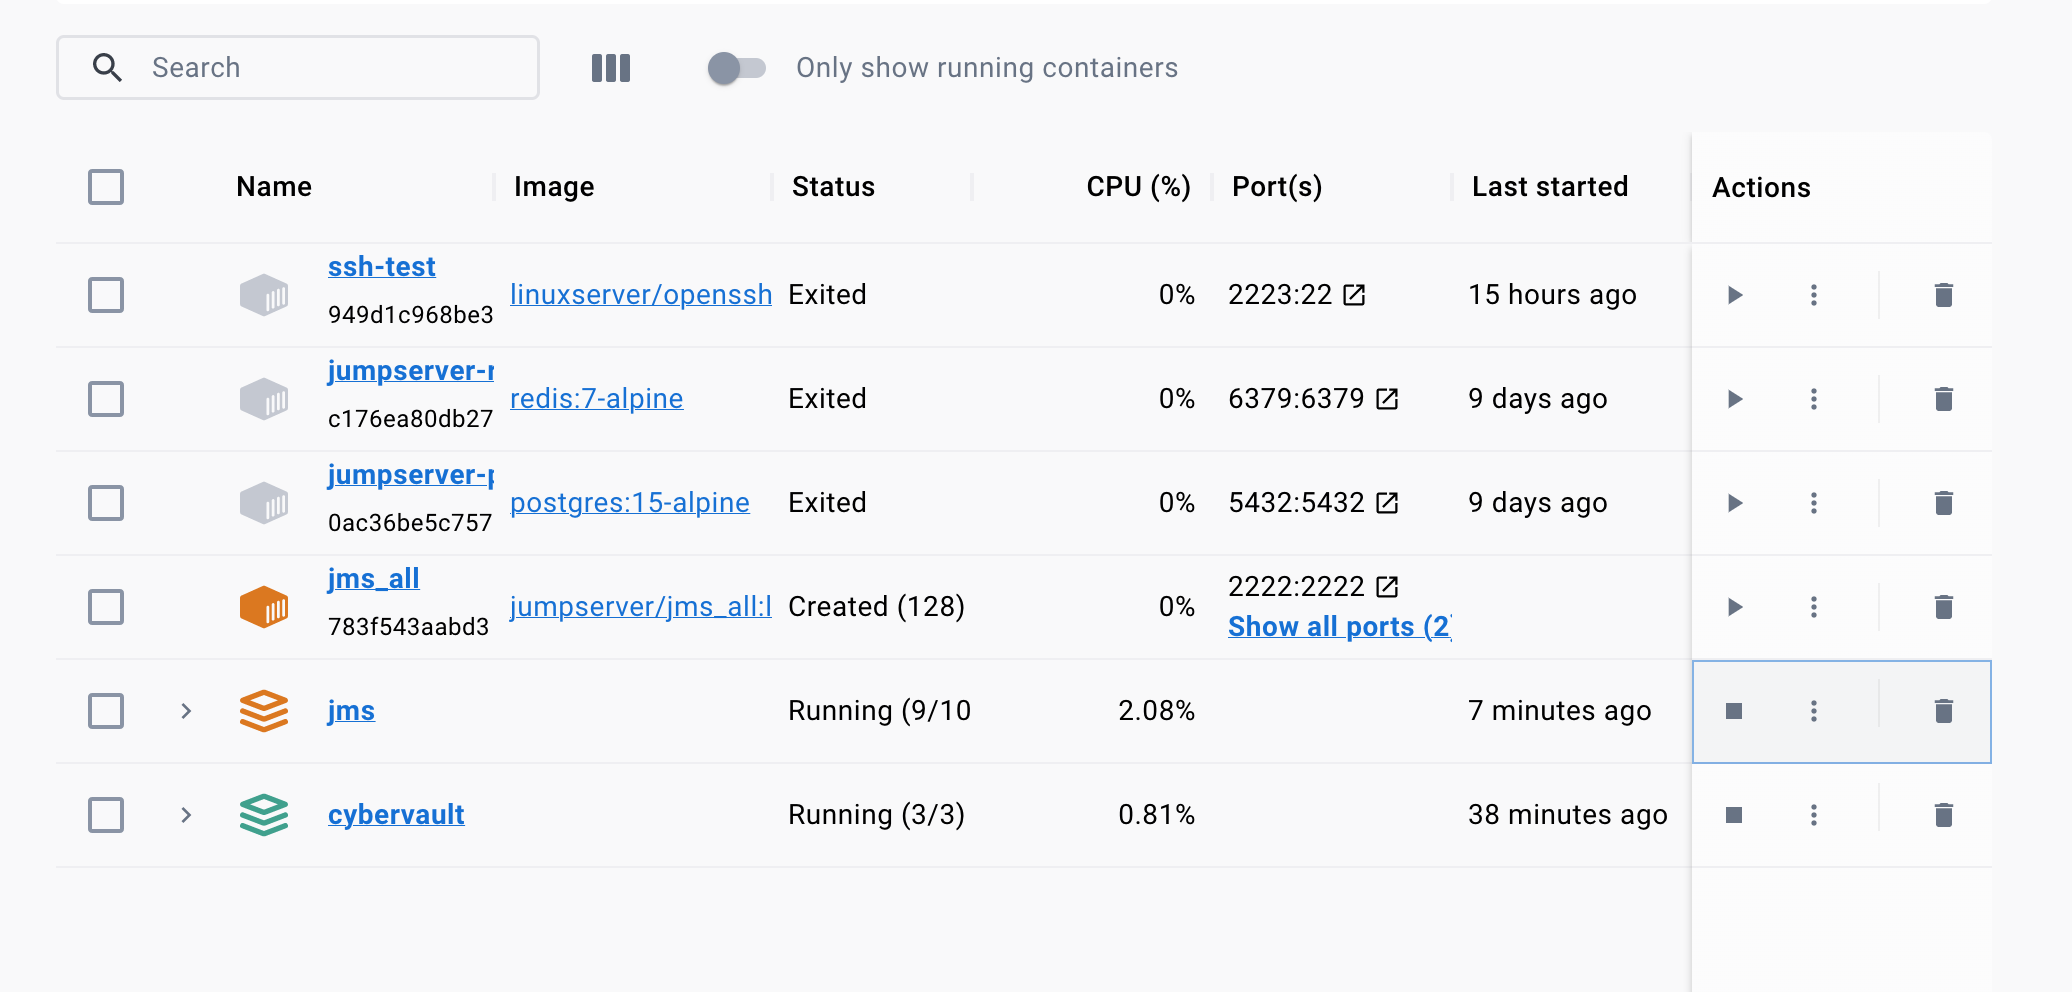
\includegraphics[width=0.92\textwidth]{docker-desktop-stacks.png}
\caption{Orchestration locale observée dans Docker Desktop : piles
\texttt{jms} (JumpServer) et \texttt{cybervault} (analyse et interface)
cohabitent sur le même hôte.}
\label{fig:deploy-docker-desktop}
\end{figure}

\begin{figure}[H]
\centering
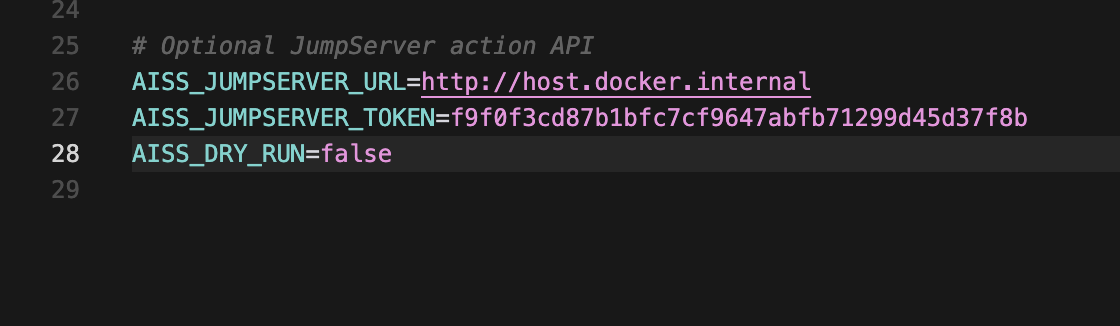
\includegraphics[width=0.88\textwidth]{env-jumpserver-api.png}
\caption{Extrait de configuration \path{.env} : URL JumpServer, jeton API et
\texttt{AISS\_DRY\_RUN=false} pour autoriser les actions réelles en
laboratoire.}
\label{fig:deploy-env-api}
\end{figure}

Le lancement typique du POC local suit trois étapes. Premièrement, démarrer
JumpServer (compose ou installateur officiel) jusqu'à l'accès à l'interface
web. Deuxièmement, lancer CyberVault par
\texttt{docker compose up -d --build} à la racine du dépôt. Troisièmement,
configurer l'intégration dans l'écran \emph{Mon PAM} (URL, jeton, e-mail
d'alerte) et vérifier \path{/health}. Cette procédure reste volontairement
guidée et mono-hôte : elle vise la reproductibilité de la démonstration, non
une haute disponibilité.

\section{Déploiement AWS et état réel de la feuille de route}

Le projet met en œuvre une preuve de concept AWS basée sur EC2. Le modèle
\path{deploy/aws/cloudformation-ec2-poc.yaml} crée un VPC
\texttt{10.42.0.0/16}, un sous-réseau public, une passerelle Internet, une
table de routage, un groupe de sécurité, une instance Ubuntu avec un volume
EBS de 40 Gio et une adresse IP élastique. Le \emph{user data} installe les
outils de base et Docker, puis écrit un témoin d'amorçage. Les sorties
fournissent l'adresse publique, une commande SSH et les URL attendues.

CloudFormation automatise l'infrastructure EC2 de base. L'opérateur exécute
ensuite \path{deploy/aws/run-poc.sh}, installe JumpServer avec son
installateur officiel, modifie sa configuration puis lance le script de
connexion. Cette approche guidée permet une preuve de concept cloud tout en
documentant explicitement les étapes manuelles. Le groupe de sécurité ouvre
22, 80, 443, 2222 et 8090 au paramètre \texttt{AllowedCidr}. La documentation
recommande une adresse d'administration en \texttt{/32} pour restreindre
l'accès, établissant les bonnes pratiques de sécurité.

Le producteur Django pour Kinesis est implémenté : il peut écrire dans un flux
existant lorsque \texttt{boto3}, la région, le nom de flux et les identifiants
sont fournis. Cette implémentation établit la base pour une extension
cloud-native. Le répertoire \path{ai-security-service/infra/} documente
l'architecture cible : Kinesis en mode à la demande, Firehose vers S3, Lambda
pour l'enrichissement et l'exécution, et DynamoDB pour les décisions, les
baselines et la configuration. Cette documentation architecturale fournit une
feuille de route claire pour l'industrialisation progressive.

\section{Frontières de confiance et sécurité de l'API}

La figure~\ref{fig:impl-deployment} synthétise le déploiement en conservant la
distinction entre éléments exécutables, capacités incomplètes et cible
d'industrialisation.

\begin{figure}[H]
\centering
\resizebox{0.98\textwidth}{!}{%
\begin{tikzpicture}[
  node distance=9mm and 12mm,
  implemented/.style={draw,rounded corners,thick,fill=cv2!12,
                      align=center,minimum width=29mm,minimum height=9mm},
  partial/.style={draw,rounded corners,thick,dashed,fill=cv4!12,
                  align=center,minimum width=29mm,minimum height=9mm},
  planned/.style={draw,rounded corners,dash dot,fill=cv5!10,
                  align=center,minimum width=29mm,minimum height=9mm},
  boundary/.style={draw,dashed,rounded corners,inner sep=5mm},
  flow/.style={-{Latex[length=2mm]},thick},
  partialflow/.style={-{Latex[length=2mm]},thick,dashed},
  plannedflow/.style={-{Latex[length=2mm]},dash dot,color=cv5}
]
\node[implemented] (jumpserver) {JumpServer\\Django + Celery};
\node[implemented, right=of jumpserver] (local) {Fichier / Redis / HTTP\\producteurs et consommateurs};
\node[implemented, below=of local] (aiss) {AISS :8090\\moteur + API HTTP};
\node[implemented, left=of aiss] (state) {Volume AISS\\JSON / JSONL};
\node[implemented, below=of jumpserver] (ec2) {EC2 + VPC + EIP\\CloudFormation};

\node[partial, right=20mm of local] (kinesis) {Kinesis\\producteur seul};
\node[planned, below=of kinesis] (firehose) {Firehose + S3\\archive planifiée};
\node[planned, right=of firehose] (lambda) {Lambda\\traitement planifié};
\node[planned, below=of lambda] (dynamo) {DynamoDB\\état planifié};

\node[boundary, fit=(jumpserver)(local)(aiss)(state)(ec2),
      label={[font=\small]above:POC sur hôte local ou EC2}] {};

\draw[flow] (jumpserver) -- (local);
\draw[flow] (local) -- (aiss);
\draw[flow] (aiss) -- (state);
\draw[flow] (ec2) -- (jumpserver);
\draw[partialflow] (jumpserver) -- (kinesis);
\draw[plannedflow] (kinesis) -- node[right,font=\scriptsize]{consommation absente} (firehose);
\draw[plannedflow] (firehose) -- (lambda);
\draw[plannedflow] (lambda) -- (dynamo);

\node[implemented, below=18mm of state, minimum width=20mm] (leg1) {implémenté};
\node[partial, right=of leg1, minimum width=20mm] (leg2) {partiel};
\node[planned, right=of leg2, minimum width=20mm] (leg3) {planifié};
\end{tikzpicture}}
\caption{Déploiement de CyberVault selon l'état attesté du dépôt. Le POC
local ou EC2 est implémenté, Kinesis est limité au producteur, et la chaîne
Firehose--S3--Lambda--DynamoDB demeure planifiée.}
\label{fig:impl-deployment}
\end{figure}

Le webhook compare le bearer token à la valeur
\texttt{AISS\_WEBHOOK\_TOKEN} lorsqu'elle est définie. Lorsqu'elle est vide,
il accepte toute requête atteignant \path{/events}. L'interface possède par
ailleurs un magasin d'utilisateurs local : les mots de passe sont dérivés par
PBKDF2-HMAC-SHA256 avec sel, les jetons sont aléatoires, expirent et sont
comparés de manière constante. Ces mesures sont utiles, mais elles ne
constituent pas une autorisation complète.

En effet, l'authentification est appliquée à certaines mutations, telles que
la connexion d'intégration, l'envoi d'un test, l'effacement de l'historique ou
le rejeu. Plusieurs lectures restent ouvertes, notamment l'état, la
configuration, les décisions, les détails et l'activité. Plus grave, la
lecture et l'écriture de \path{/api/config} ne vérifient pas systématiquement
l'utilisateur. Les utilisateurs, sessions, jetons JumpServer et paramètres
sont enregistrés dans des fichiers locaux en clair ; le navigateur conserve
son bearer dans \texttt{localStorage}. Une redirection côté client ne protège
pas une route serveur. L'authentification doit donc être qualifiée de
partielle.

Le client de contrôle JumpServer transmet un jeton statique et l'en-tête
d'organisation attendu pour demander le verrouillage ou l'arrêt d'une
session. Il faut lui attribuer un compte de service au privilège minimal,
séparer son secret des journaux et renouveler le jeton. Le port AISS doit
rester sur un réseau restreint, derrière un proxy inverse qui assure TLS,
limitation de débit, taille maximale des requêtes et journalisation. Dans
l'état présent, le service n'offre ni TLS natif, ni protection CSRF homogène,
ni rôles, ni scellement des journaux.

Une divergence de configuration peut encore affecter le mode simulation. Les
variables d'environnement interprètent correctement
\texttt{AISS\_DRY\_RUN=false}, et le processeur privilégie désormais cette
valeur d'environnement lorsque la simulation est exigée comme garde-fou. En
pratique de laboratoire, la désactivation effective du mode test nécessite
néanmoins de recréer le conteneur \texttt{backend} après modification du
fichier \path{.env}, faute de quoi le processus conserve l'ancienne valeur en
mémoire. L'écran d'état et la configuration utilisateur doivent rester alignés
avec cette source pour éviter toute ambiguïté avant une action réelle.

\section{Interfaces du prototype de démonstration}

Outre les diagrammes d'architecture, la démonstration s'appuie sur des
interfaces web qui rendent visibles l'intégration et le contrôle. La
figure~\ref{fig:ui-jumpserver-login} présente la page d'authentification de
JumpServer, point d'entrée du bastion sur l'instance locale. Après connexion,
l'administrateur peut compléter son profil (figure~\ref{fig:ui-jumpserver-profile}),
notamment l'adresse e-mail et les options MFA, avant d'ouvrir des sessions
privilégiées.

\begin{figure}[H]
\centering
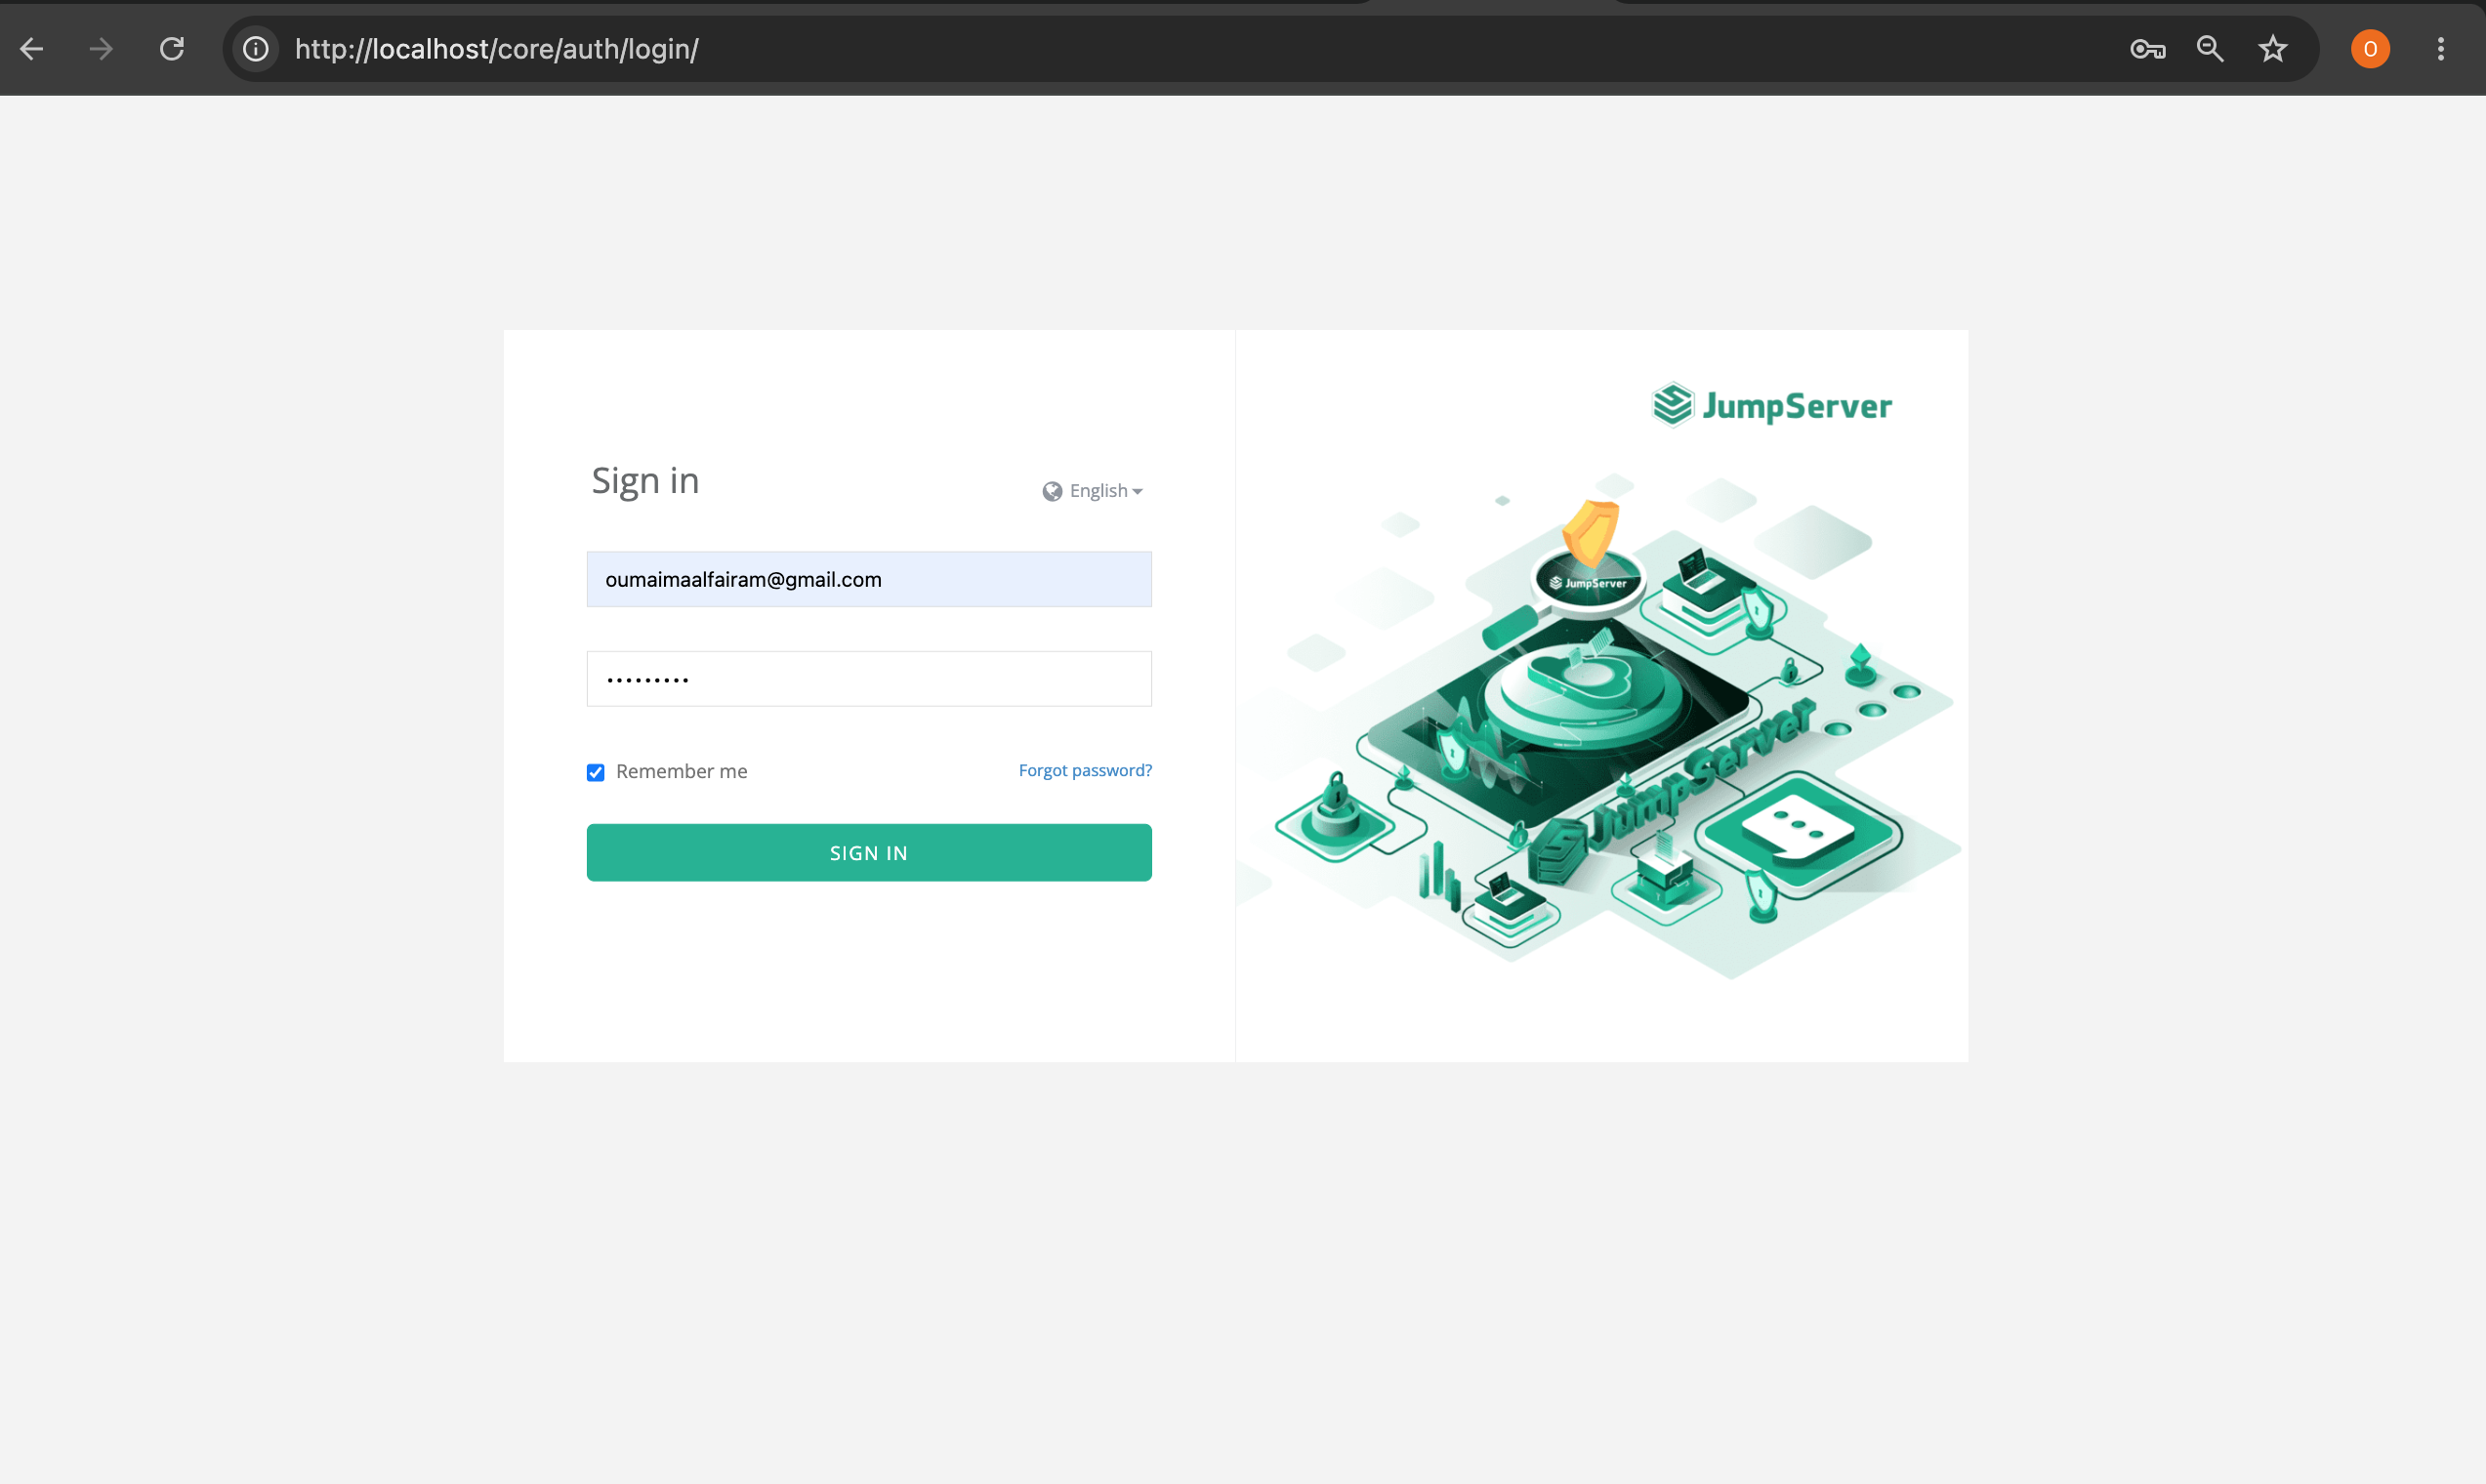
\includegraphics[width=0.88\textwidth]{jumpserver-login.png}
\caption{Interface d'authentification JumpServer (instance locale
\texttt{localhost}).}
\label{fig:ui-jumpserver-login}
\end{figure}

\begin{figure}[H]
\centering
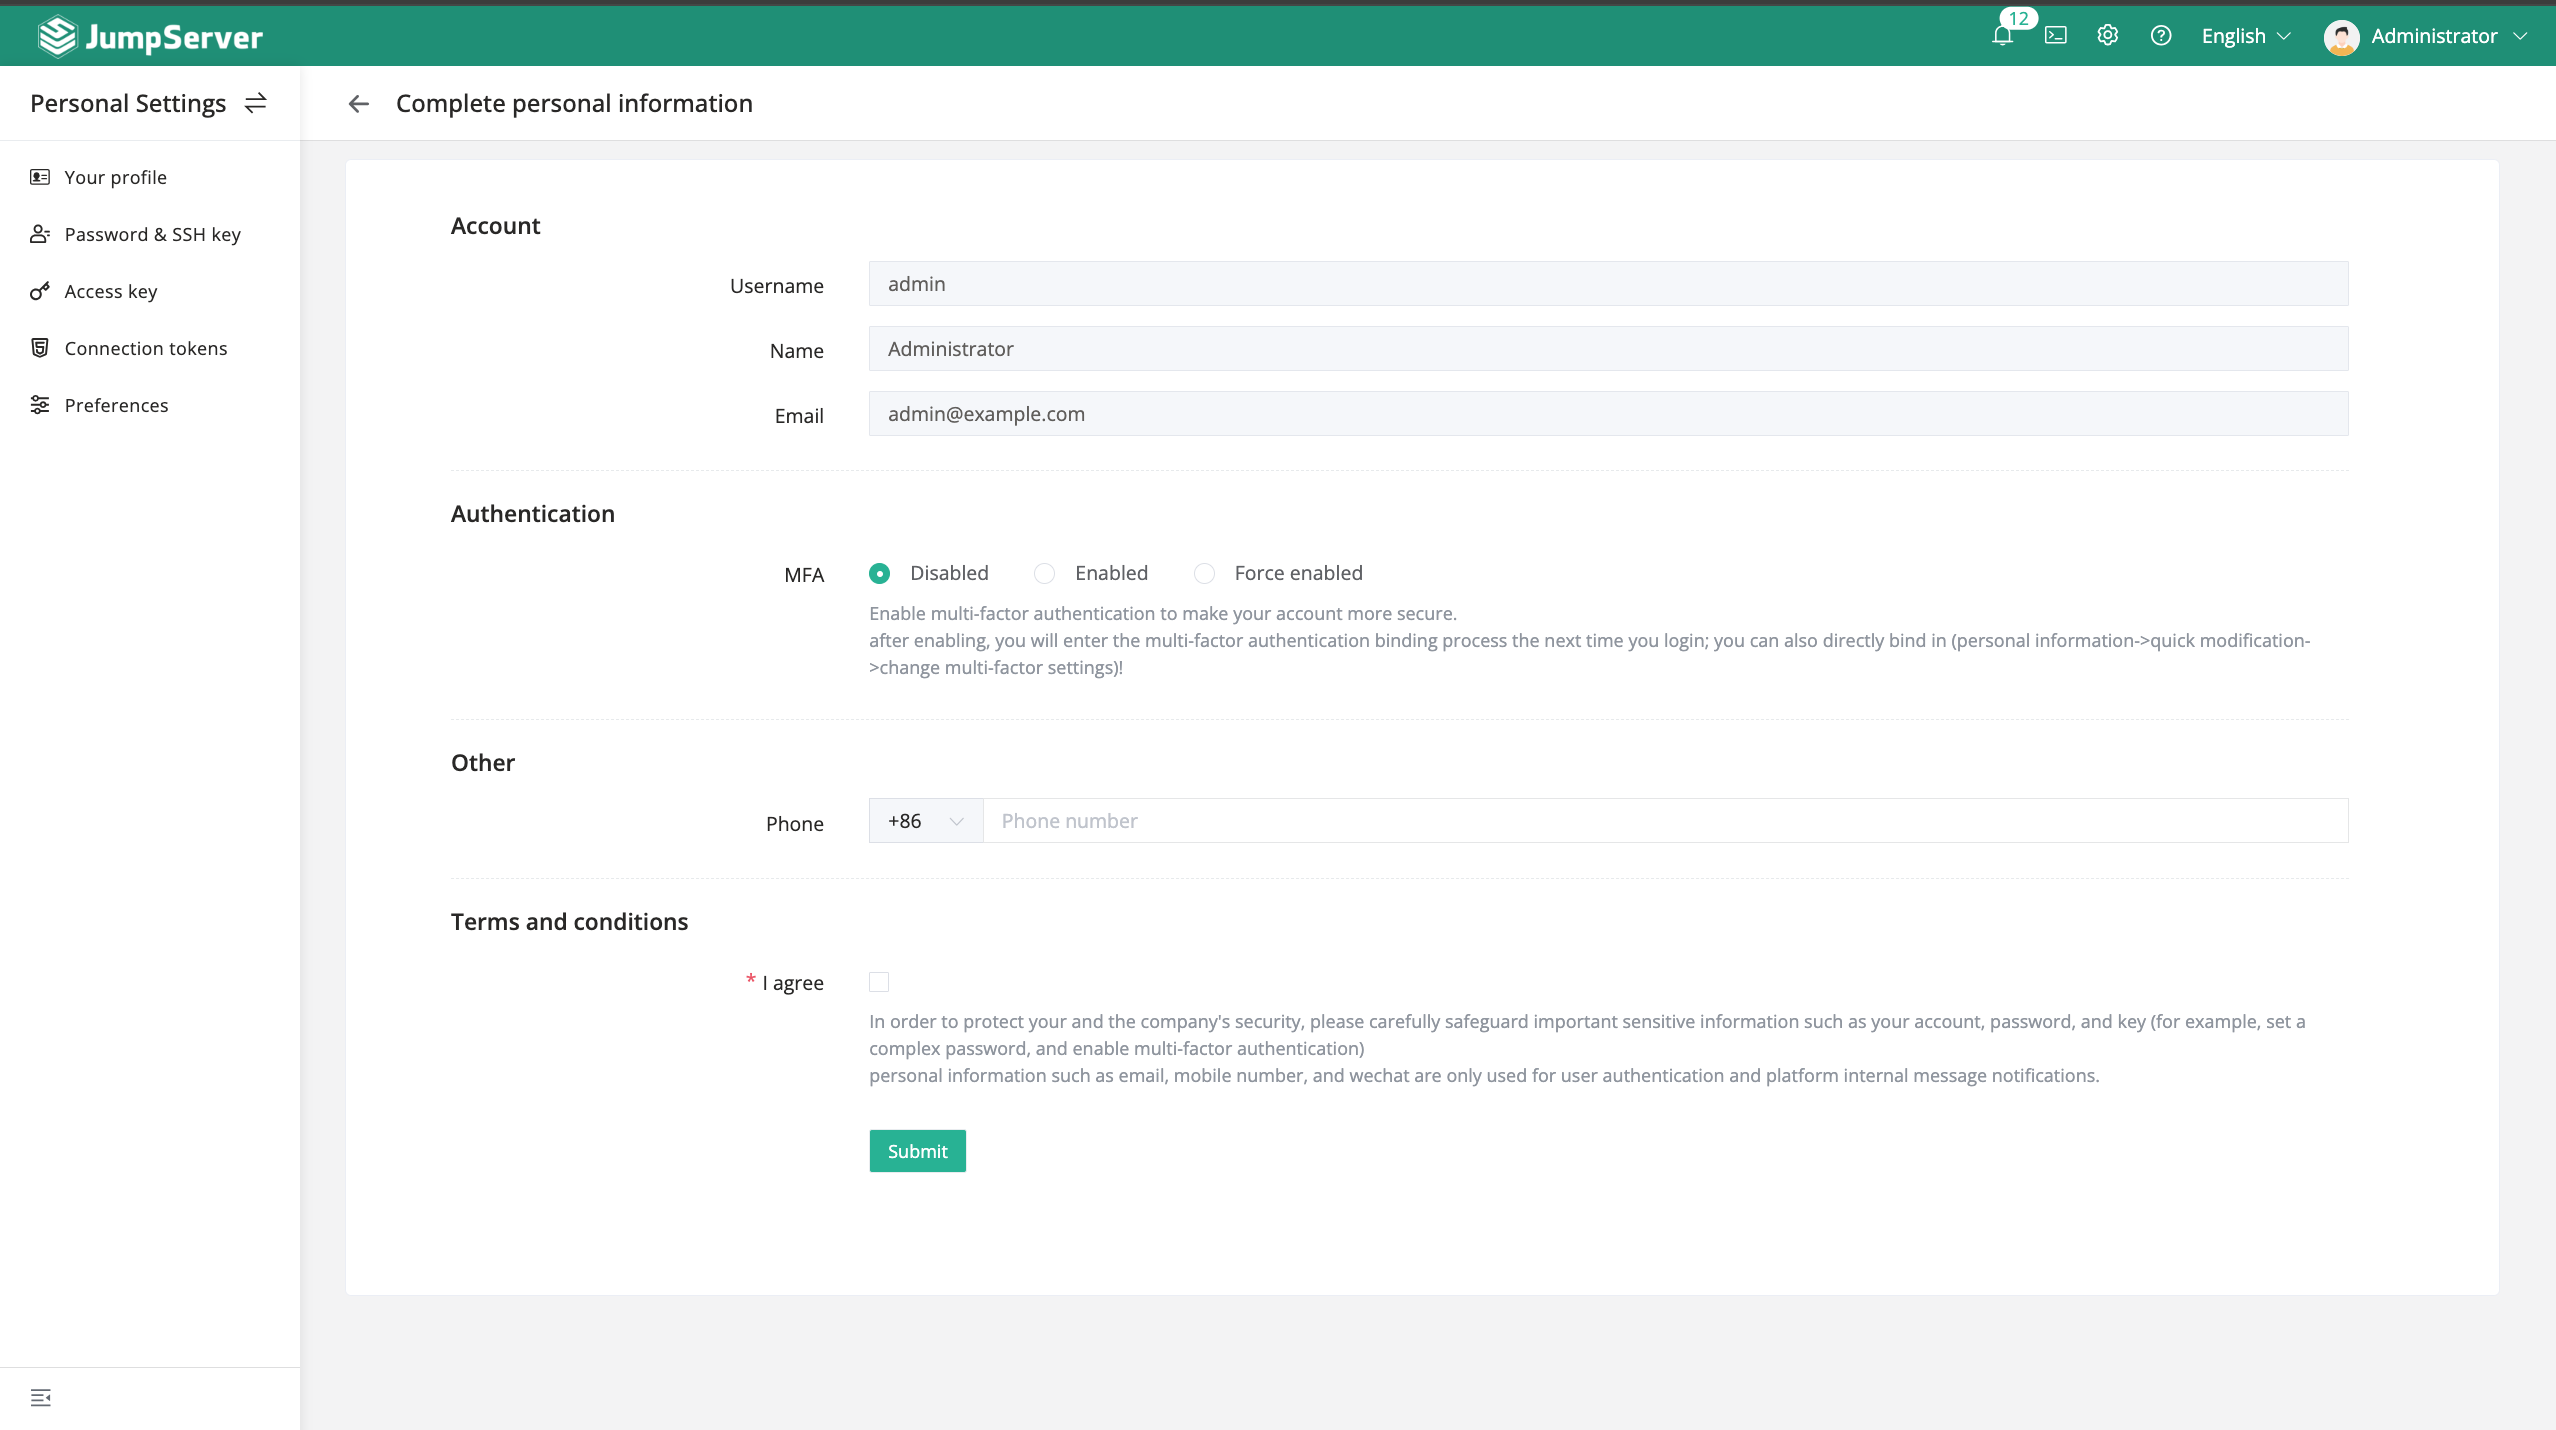
\includegraphics[width=0.88\textwidth]{jumpserver-profile.png}
\caption{Complétion du profil administrateur JumpServer : identité, e-mail et
options d'authentification multifacteur.}
\label{fig:ui-jumpserver-profile}
\end{figure}

Du côté CyberVault, le premier compte créé devient administrateur de
l'instance (figure~\ref{fig:ui-cybervault-signup}). L'écran \emph{Mon PAM}
(figure~\ref{fig:ui-mon-pam}) centralise ensuite le branchement JumpServer
(URL et jeton API) et la configuration des alertes e-mail. Ces écrans ne
remplacent pas le bastion : ils exposent la couche d'analyse et de notification
pour l'opérateur SOC.

\begin{figure}[H]
\centering

\includegraphics[width=0.88\textwidth]{cybervault-signup.png}
\caption{Création du compte CyberVault : le premier compte devient
administrateur de l'instance ; le panneau gauche rappelle les capacités
(détection temps réel, dry-run, intégration cloud).}
\label{fig:ui-cybervault-signup}
\end{figure}

\begin{figure}[H]
\centering

\includegraphics[width=0.88\textwidth]{cybervault-mon-pam.png}
\caption{Écran \emph{Mon PAM} : intégration JumpServer et paramétrage des
alertes administrateur par e-mail.}
\label{fig:ui-mon-pam}
\end{figure}

\section{Transition vers le temps réel}

Le déploiement réalisé permet d'instrumenter JumpServer, de transporter les
événements par trois chemins complets (fichier, Redis, HTTP), d'exécuter AISS
et de conserver un état inspectable. Cette architecture établit la faisabilité
de bout en bout sur un poste ou une instance unique, démontrant ainsi les
principes d'intégration.

Une industrialisation progressive nécessiterait une image reproductible
incluant les ressources statiques, un registre d'artefacts contrôlé, une
authentification serveur systématique et une topologie réseau explicite. La
persistance pourrait évoluer vers un stockage transactionnel, et la branche
AWS compléter le consommateur Kinesis pour introduire progressivement
l'archivage et l'état gérés.

La section suivante examine le fonctionnement en temps réel : le comportement
observable du chemin implémenté depuis l'événement JumpServer jusqu'à la
décision AISS. Cette transition préserve la distinction entre la mécanique
d'intégration et de déploiement établie ici, et l'étude de son fonctionnement
lors de l'arrivée effective des événements.



\section{Fonctionnement en temps réel}
\label{sec:impl-realtime}

\section{Principe d'exécution et garanties effectives}

Le fonctionnement en temps réel de CyberVault relie l'activité observée dans
JumpServer à une décision de sécurité inspectable. Le terme « temps réel »
désigne un traitement événementiel déclenché après l'activité. La chaîne est
asynchrone jusqu'à l'ingestion, puis synchrone dans le processus consommateur
pour l'analyse d'un événement. Elle suit un ordre déterminé : hook JumpServer,
tâche Celery, transport, ingestion, décodage, enrichissement, règles et UEBA,
modèles tabulaires conditionnels, modèles profonds expérimentaux facultatifs,
fusion, explicabilité conditionnelle, choix d'une réponse, exécution, mise à
jour comportementale et persistance. Cet ordre architectural garantit que
chaque étape prépare les invariants exigés par la suivante.

L'architecture préserve JumpServer comme autorité pour l'authentification,
l'autorisation, l'enregistrement et le contrôle des sessions. CyberVault est
un consommateur secondaire de télémétrie structurée. Cette séparation offre
une intégration résiliente : une indisponibilité de CyberVault ne bloque pas
le chemin nominal du bastion. Réciproquement, une décision CyberVault ne
produit un effet sur une session que si l'action est prise en charge, si les
paramètres de contrôle sont présents et si le mode simulation est désactivé,
offrant un contrôle explicite sur les actions automatisées. La chaîne
privilégie le découplage et l'inspectabilité.

\section{De JumpServer à l'entrée du processeur}

\subsection{Hook JumpServer : observer après l'opération métier}

Le point de départ est un hook placé au plus près de l'activité pertinente.
Les récepteurs Django observent notamment la création et la fin d'une session,
la réussite ou l'échec d'une connexion, le cycle de vie d'un compte de service,
le stockage de commandes et les violations d'ACL de commandes. Les événements
de commande sont émis après leur stockage groupé réussi, et le cycle de vie
d'un compte est transmis après la création du journal JumpServer. Ce
positionnement est important : CyberVault reçoit la description d'une
opération déjà reconnue par le bastion, au lieu d'intercepter et de modifier
son chemin métier.

Le hook construit une enveloppe contenant, selon le type disponible,
l'identifiant d'événement, l'horodatage UTC, l'utilisateur, la session,
l'actif, le compte cible, l'adresse distante et une charge utile telle qu'une
commande ou un niveau ACL. Cette représentation commune permet aux étapes
ultérieures de traiter des sources hétérogènes selon un contrat stable. La
contribution du hook est donc double : sélectionner les points d'observation
ayant une signification de sécurité et préserver la provenance JumpServer.
Il ne garantit toutefois pas que toute activité système soit visible : seules
les opérations instrumentées et les données structurées fournies par le
bastion entrent dans l'analyse.

\subsection{Celery : sortir les entrées-sorties du chemin JumpServer}

Lorsque \texttt{AI\_SECURITY\_ENABLED} est actif, le répartiteur délègue la
publication à \texttt{publish\_security\_events\_task.delay()}. La construction
de l'événement reste dans le processus de requête ou de signal, tandis que le
worker Celery réalise les entrées-sorties externes. Cette séparation évite
qu'une latence HTTP, Redis ou Kinesis ne prolonge directement le traitement
interactif de JumpServer. Elle apporte également un point unique pour choisir
le transport et consigner les erreurs de publication.

Cette transmission suit un modèle \emph{best-effort}. Le choix asynchrone
protège la disponibilité du bastion et offre un découplage efficace entre
les responsabilités.

\subsection{Transport : quatre sorties, trois chemins d'entrée}

La tâche Celery sélectionne le transport configuré. Le mode fichier ajoute un
objet JSON par ligne ; il facilite l'observation et le rejeu local, sans
verrouillage interprocessus ni synchronisation forcée sur disque. Redis publie
sur un canal Pub/Sub ; il réduit le couplage, mais ne fournit ni persistance ni
acquittement. HTTP envoie un lot sous la forme
\texttt{\{"events":[...]\}} avec délai d'expiration et jeton bearer
facultatif ; une réponse non \(2xx\) devient une erreur de publication.
Kinesis appelle \texttt{put\_record} pour chaque événement et utilise la
session ou l'événement comme clé de partition, ce qui peut préserver l'ordre
dans une partition, sous les garanties du service.

Le producteur Kinesis est implémenté : il appelle \texttt{put\_record} pour
chaque événement et utilise la session ou l'événement comme clé de partition,
préservant ainsi l'ordre dans une partition sous les garanties du service.
Cette implémentation établit la base pour une architecture cloud-native. Le
consommateur Kinesis appartient à la feuille de route d'industrialisation,
documentée dans le répertoire \path{ai-security-service/infra/}. Cette
approche par étapes distingue explicitement les composants implémentés des
extensions planifiées.

\subsection{Ingestion et contrôle syntaxique : établir une frontière minimale}

Le consommateur fichier lit les nouvelles lignes, avec un sondage périodique,
et ignore les lignes JSON mal formées. Le consommateur Redis s'abonne au canal
et décode chaque message. En parallèle, le serveur HTTP accepte un événement
unitaire ou une liste sur \path{/events}. Le webhook ne vérifie le bearer que
si \texttt{AISS\_WEBHOOK\_TOKEN} est défini ; une valeur vide ne constitue
donc pas une authentification. L'ingestion transforme ces trois formes en un
appel commun au processeur, ce qui évite que le choix du transport modifie la
logique de détection.

Le transport vérifie que la charge est un objet JSON décodable, puis transmet
le dictionnaire au processeur. Celui-ci enrichit directement les champs
disponibles et applique plusieurs valeurs par défaut, garantissant ainsi une
syntaxe exploitable. Le schéma formel \path{schemas/security_event.json}
documente le contrat attendu ; une validation formelle avant l'enrichissement
renforcerait la frontière de confiance pour un durcissement opérationnel.

\section{Construction du contexte et évaluation ordonnée}

\subsection{Enrichissement : replacer l'observation dans son historique}

\texttt{FeatureStore.enrich()} est exécuté avant tous les détecteurs. Il
maintient, par session, jusqu'à cinquante commandes, un nombre d'événements et
le dernier horodatage, ainsi qu'un cumul de commandes par utilisateur.
L'événement enrichi reçoit notamment les volumes de session, le total
utilisateur, les dix commandes récentes, l'heure UTC, l'adresse normalisée et
les indicateurs ACL. Cette étape rend calculables la vélocité, la nouveauté et
les motifs dépendant d'une séquence récente, impossibles à déduire de la seule
ligne courante.

L'enrichissement transforme une télémétrie ponctuelle en observation
contextuelle. Il précède nécessairement le score, garantissant ainsi que tous
les moteurs opèrent sur des informations cohérentes. Son état JSON offre une
persistance inspectable adaptée au prototype mono-processus. Une extension
distribuée nécessiterait un stockage transactionnel avec coordination entre
consommateurs.

\subsection{Règles puis UEBA : conserver le connu et mesurer l'écart}

Le moteur de règles examine d'abord des connaissances explicites : violation
d'ACL, commande destructive, volume de commandes élevé et niveau ACL
critique. Chaque motif possède une sévérité, et le score \(r_R\) est le maximum
des règles activées. Cette méthode conserve sans dilution un interdit connu :
une commande destructive ne devient pas bénigne parce que d'autres moteurs
sont silencieux. Elle fournit aussi un motif directement auditable, mais ne
couvre que les expressions et seuils configurés.

L'UEBA évalue ensuite l'événement contre le profil de l'utilisateur. Après
cinq observations apprises, il recherche une heure, une adresse, un actif ou
un compte inhabituel, une vélocité excessive, des échecs de connexion, une
rafale d'échecs ou une dispersion sur de nombreux actifs. Son score \(r_B\)
est également une sévérité maximale. Sa contribution est de détecter un usage
atypique même lorsque chaque commande reste légitime. Avant maturité, il
signale explicitement son initialisation, préservant ainsi la distinction entre
détection fondée sur un profil établi et détection en phase d'apprentissage.
Les réseaux d'entreprise configurés peuvent ramener son score à zéro,
offrant ainsi un contrôle explicite sur la confiance accordée aux réseaux
internes ; un réglage plus fin par indicateur comportemental renforcerait la
granularité du contrôle.

\subsection{IF et RF conditionnelles : exploiter les artefacts disponibles}

Le vecteur tabulaire de douze caractéristiques est construit après
l'enrichissement. La Forêt d'isolation (IF) mesure l'isolement d'une
observation par rapport aux normales d'entraînement ; elle apporte un signal
de nouveauté sans nécessiter un catalogue complet d'attaques. La Forêt
aléatoire (RF) exploite au contraire les étiquettes et apprend des interactions
non linéaires entre indicateurs, volumes et contexte. Lorsque les deux modèles
sont chargés, leur composante commune vaut
\[
 r_M=0.40\,r_M^{\mathrm{IF}}+0.60\,r_M^{\mathrm{RF}}.
\]
Si un seul modèle existe, son score est utilisé ; si aucun n'existe,
\(r_M=0\) est accompagné d'un statut explicite d'indisponibilité, préservant
ainsi la distinction entre absence de modèle et faible risque détecté.

L'architecture prévoit l'entraînement et l'injection contrôlée des poids de
modèles. Des métadonnées JSON documentent le schéma attendu. L'interface de
dégradation permet aux règles et à l'UEBA de continuer l'évaluation en
l'absence de modèles appris, garantissant ainsi une détection de base même sans
artefacts d'apprentissage. Cette architecture en couches offre une résilience
opérationnelle : le système reste fonctionnel avec des capacités réduites
plutôt que de s'arrêter complètement.

\subsection{LSTM et GNN : extensions expérimentales facultatives}

Après les moteurs tabulaires, le processeur peut appeler une branche
séquentielle LSTM puis une branche de graphe GNN. La première vise les motifs
ordonnés de commandes ou d'événements ; la seconde vise les relations entre
utilisateurs, sessions et actifs. Leur intérêt est de représenter
respectivement la dynamique temporelle et la structure relationnelle que le
vecteur fixe résume de manière limitée.

Ces deux branches sont expérimentales et facultatives. Elles produisent un
signal lorsque leurs dépendances et artefacts sont disponibles. Leur présence
dans le code établit l'architecture extensible : elles sont exécutées après
IF/RF pour préserver l'ordre d'orchestration, et leur absence n'interrompt ni
les moteurs déterministes ni l'UEBA. Cette architecture en couches permet
l'intégration progressive de nouveaux moteurs sans perturber les composants
existants.

\subsection{Fusion : préserver le signal le plus sévère}

Les sorties disponibles sont fusionnées seulement après l'évaluation de tous
les moteurs :
\[
 r=\max\{r_R,r_B,r_M,r_{\mathrm{LSTM}},r_{\mathrm{GNN}}\}.
\]
La confiance est agrégée séparément par maximum, les motifs sont concaténés et
le résultat indique quels moteurs ont effectivement contribué. Le maximum
répond à l'asymétrie du contrôle privilégié : un indice fort ne doit pas être
abaissé par la moyenne de plusieurs moteurs absents ou silencieux. Cette
contribution est conservatrice et lisible, mais elle transmet également le
bruit du moteur le plus sensible ; le score fusionné n'est ni une probabilité
calibrée ni une preuve causale.

\subsection{XAI RF conditionnelle : expliquer sans décider}

Une explication est tentée après la fusion des scores appris lorsque le seuil
configuré est atteint et lorsque RF ainsi qu'une matrice de fond existent.
TreeSHAP et LIME peuvent alors associer aux caractéristiques des contributions
locales, conservées avec la décision. Cette position dans la chaîne évite que
l'explication influence le risque : elle sert à examiner une prédiction déjà
produite.

L'XAI est ciblée sur RF, le modèle supervisé tabulaire. Elle fournit des
contributions locales pour ce composant, complétées par les motifs nommés des
règles et de l'UEBA pour le reste de la chaîne. Cette portée est un choix de
conception : TreeSHAP et LIME offrent des garanties théoriques adaptées à RF.
Lorsque RF ou la matrice de référence sont indisponibles, la décision se
poursuit sans explication locale, ce qui préserve la continuité du service. Les
contributions SHAP documentent une prédiction et offrent une aide concrète à
l'investigation.

\section{De la décision à l'état visible}

\subsection{Seuils et repli : sélectionner une action admissible}

Le risque fusionné est d'abord projeté sur une table de seuils. Un risque
inférieur à \(0.25\) conduit à l'absence d'action ; de \(0.25\) à \(0.55\), à
la journalisation ; de \(0.55\) à \(0.75\), à l'alerte analyste ; de \(0.75\)
à \(0.90\), au verrouillage ; à partir de \(0.90\), à l'arrêt. Cette
correspondance rend le comportement ordinaire prévisible et auditable.

L'arrêt n'est admissible ni pour un compte protégé ni lorsque la confiance est
inférieure à \(0.70\), préservant ainsi la disponibilité des comptes critiques.
Si le candidat viole une contrainte, un repli scalarisé énumère les actions
autorisées et minimise un coût combinant risque résiduel, perturbation
opérationnelle et fatigue. Il garantit ainsi une décision unique et
admissible. Les coefficients sont configurés et documentés, offrant une base
pour l'ajustement selon les priorités opérationnelles. Le paramètre de nombre
maximal d'arrêts par utilisateur et par heure existe dans la configuration,
fournissant un contrôle supplémentaire pour une extension future du solveur.

\subsection{Journal, notification et action : distinguer intention et effet}

\texttt{ActionExecutor} détermine d'abord le résultat d'exécution. Pour
\texttt{LOCK\_SESSION} ou \texttt{KILL\_SESSION} hors simulation, il tente
l'appel JumpServer puis écrit le journal JSONL contenant contexte, scores,
motifs, explication, action et résultat. Cette trace rend la décision
consultable et auditable. L'ordre actuel tente l'effet puis persiste le
résultat ; une écriture préalable ou transactionnelle renforcerait la
garantie pour un durcissement opérationnel.

\subsubsection{Alertes par e-mail}

Une alerte e-mail est tentée lorsque trois conditions sont réunies : les
notifications e-mail sont activées dans la configuration utilisateur, une
adresse administrateur est renseignée (écran \emph{Mon PAM},
figure~\ref{fig:ui-mon-pam}), et la décision dépasse le seuil d'alerte (action
autre que la simple journalisation, ou score de risque élevé). Le message
contient le score de risque, l'action retenue, l'utilisateur, l'IP source,
l'actif, le compte, la commande observée, l'identifiant de session, les motifs
principaux et un lien vers le tableau de bord. Chaque tentative est archivée
dans \path{alert_outbox.jsonl} ; les succès sont dédupliqués sur vingt-quatre
heures afin de limiter la fatigue. Les exceptions SMTP sont absorbées pour ne
pas interrompre le flux d'analyse, préservant ainsi la disponibilité du
système. Ce canal fournit une notification immédiate pour que
l'administrateur SOC réagisse hors de l'interface web.

Les contrôles JumpServer implémentés sont le verrouillage et l'arrêt d'une
session. Ils exigent un identifiant de session, une URL, un client et un jeton
valides. Le mode \emph{dry-run} est la valeur sûre par défaut : tant qu'il
reste actif, l'exécuteur décrit ce qui serait fait sans modifier la session,
offrant ainsi un contrôle explicite avant toute action automatisée. La
création de ticket est documentée comme statut, établissant la base pour une
intégration future. Le journal atteste d'une décision logicielle ; l'effet
JumpServer et la livraison SMTP sont conditionnels à la disponibilité des
canaux respectifs.

\subsection{Mise à jour UEBA, persistance et tableau de bord}

La mise à jour du profil intervient après la décision et l'exécution, jamais
avant. L'événement n'alimente la référence que si
\[
 r\leq 0.40.
\]
Cette porte réduit le risque d'apprendre immédiatement un comportement déjà
jugé suspect. Elle permet au profil de suivre progressivement l'activité
considérée comme faible risque, mais ne supprime pas l'empoisonnement lent :
une attaque qui reste sous le seuil peut encore être incorporée.

Enfin, \texttt{FeatureStore}, \texttt{BaselineStore}, les décisions et les
états de notification sont persistés dans des fichiers JSON ou JSONL. Le
tableau de bord et l'API relisent ces données pour afficher événements,
scores, motifs, statuts et détails. Ils constituent une surface locale
d'investigation et d'export ; ils ne forment \textbf{ni un SIEM, ni un
système de ticketing}. Aucun connecteur SIEM ni création effective de ticket
n'est présent. Les statuts affichés reflètent les traitements et tentatives
de CyberVault, sous les limites de la persistance non transactionnelle et,
pour l'image de conteneur auditée, de fichiers statiques du tableau de bord
non copiés.

La séquence complète des interactions est placée auprès du diagramme de
classes, à la Figure~\ref{fig:impl-sequence}. Cette proximité relie les
responsabilités statiques des composants à l'ordre de leurs appels. Le présent
chapitre en développe la sémantique opérationnelle ; le parcours illustré
ci-dessous et le pseudocode qui suit en fournissent la traduction concrète
puis algorithmique.

\subsection{Parcours illustré d'un événement destructeur}

Pour rendre tangible la chaîne précédente, la validation de laboratoire a
rejoué un scénario complet sur un actif SSH de démonstration. La
figure~\ref{fig:realtime-session-before} montre une session JumpServer
ouverte sur \texttt{lab-server} : le terminal web affiche le prompt et
l'identité de l'opérateur sous forme de filigrane d'audit. La
figure~\ref{fig:realtime-command} capture ensuite la saisie d'une commande
destructrice de laboratoire (\texttt{rm -rf /tmp/demo-lab}), point de départ
de l'événement \texttt{command.ingested}.

\begin{figure}[H]
\centering
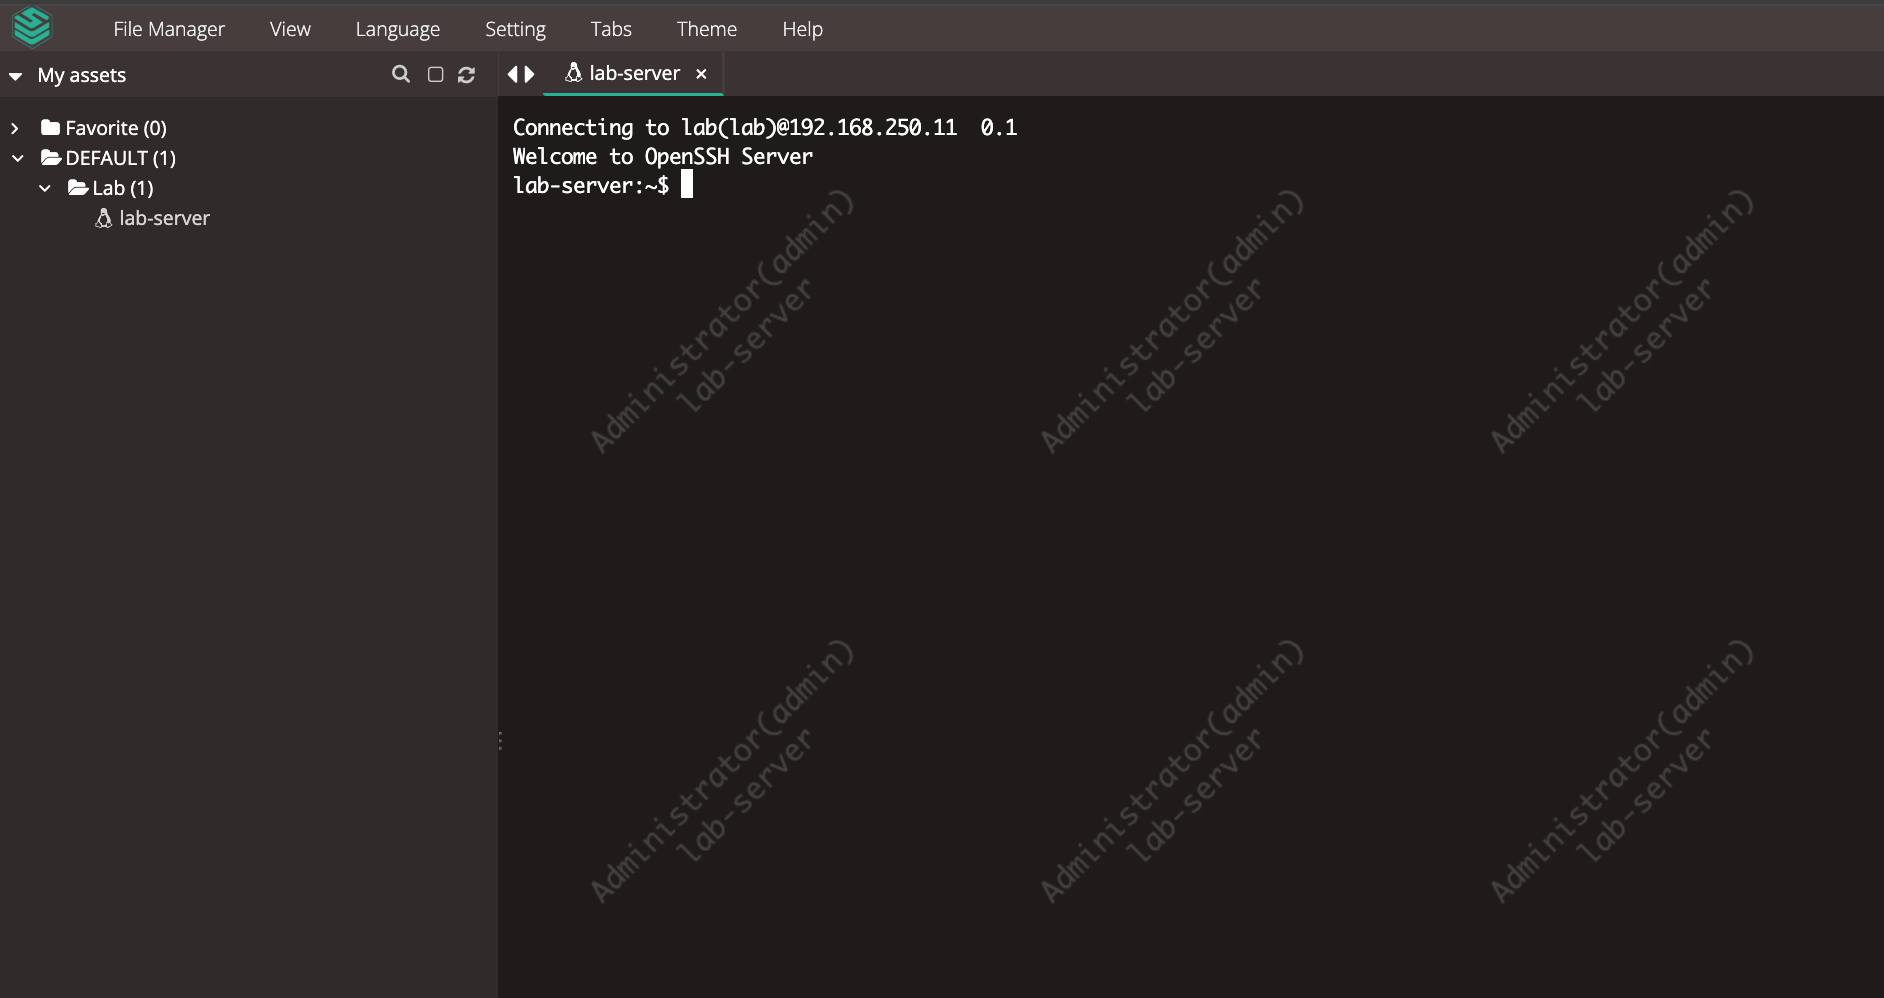
\includegraphics[width=0.88\textwidth]{session-before.png}
\caption{Session privilégiée active dans le terminal web JumpServer
(\texttt{lab-server}) avant l'intervention.}
\label{fig:realtime-session-before}
\end{figure}

\begin{figure}[H]
\centering
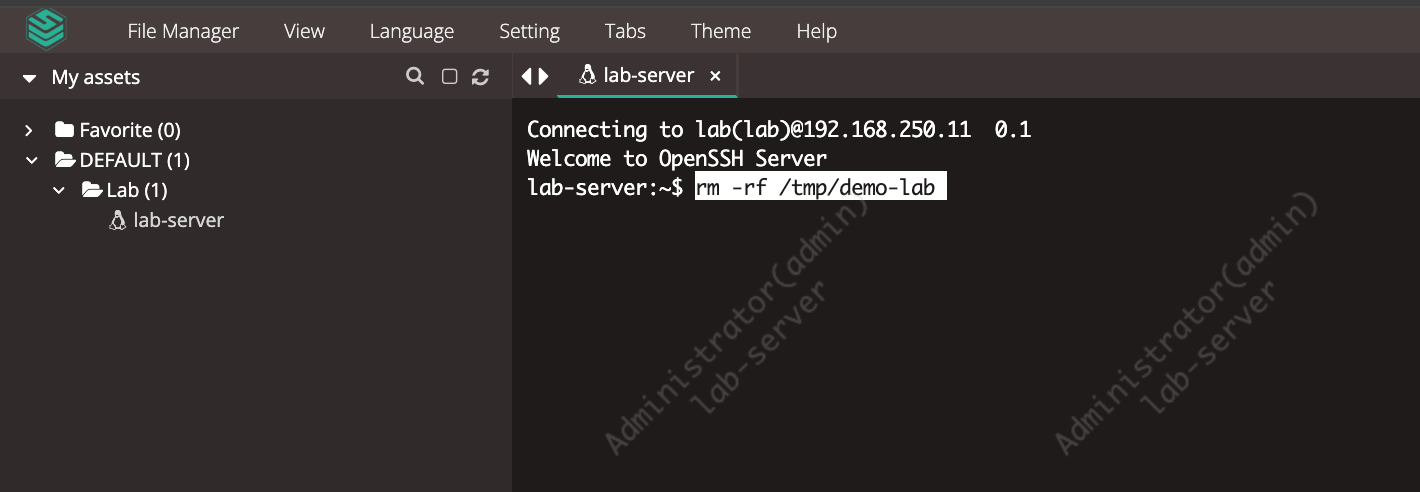
\includegraphics[width=0.78\textwidth]{session-command.png}
\caption{Commande destructrice saisie dans la session surveillée : déclencheur
de l'événement analysé par CyberVault.}
\label{fig:realtime-command}
\end{figure}

Une fois l'événement ingéré, le processeur enrichit le contexte, évalue les
moteurs disponibles, fusionne les scores et sélectionne une action. Hors mode
simulation, l'exécuteur demande à JumpServer l'arrêt de la session. La
figure~\ref{fig:realtime-session-after} montre le résultat visible côté
bastion : le message rouge \emph{Terminated by admin} et la fermeture de la
connexion WebSocket. En parallèle, le tableau de bord CyberVault
(figure~\ref{fig:ui-decisions}) journalise la décision : utilisateur, actif,
niveau de risque, action retenue (par exemple \emph{Couper session}) et
raison principale (\emph{Commande destructrice}). L'interface se rafraîchit
périodiquement afin d'afficher les nouvelles lignes sans intervention manuelle
systématique.

\begin{figure}[H]
\centering
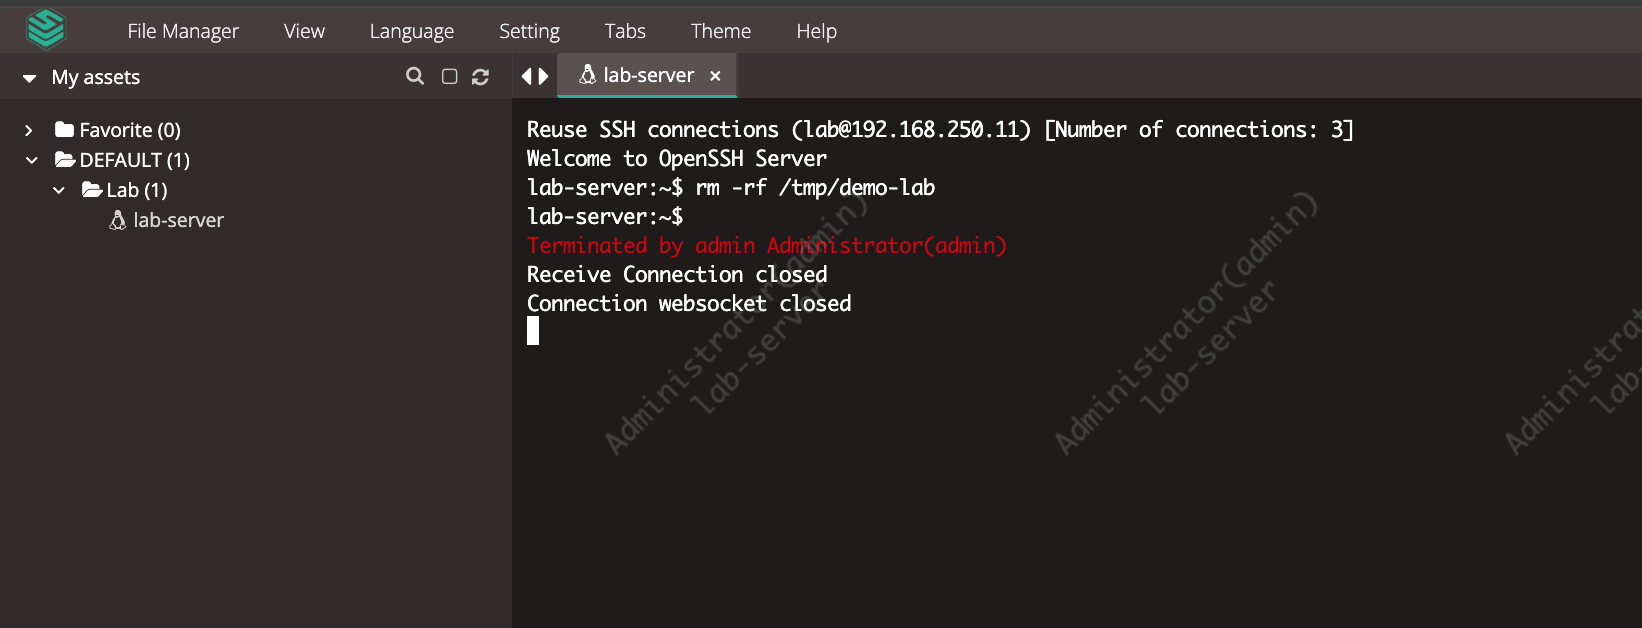
\includegraphics[width=0.88\textwidth]{session-after-kill.png}
\caption{Session JumpServer terminée après décision CyberVault : message
\emph{Terminated by admin} et fermeture de la connexion.}
\label{fig:realtime-session-after}
\end{figure}

\begin{figure}[H]
\centering
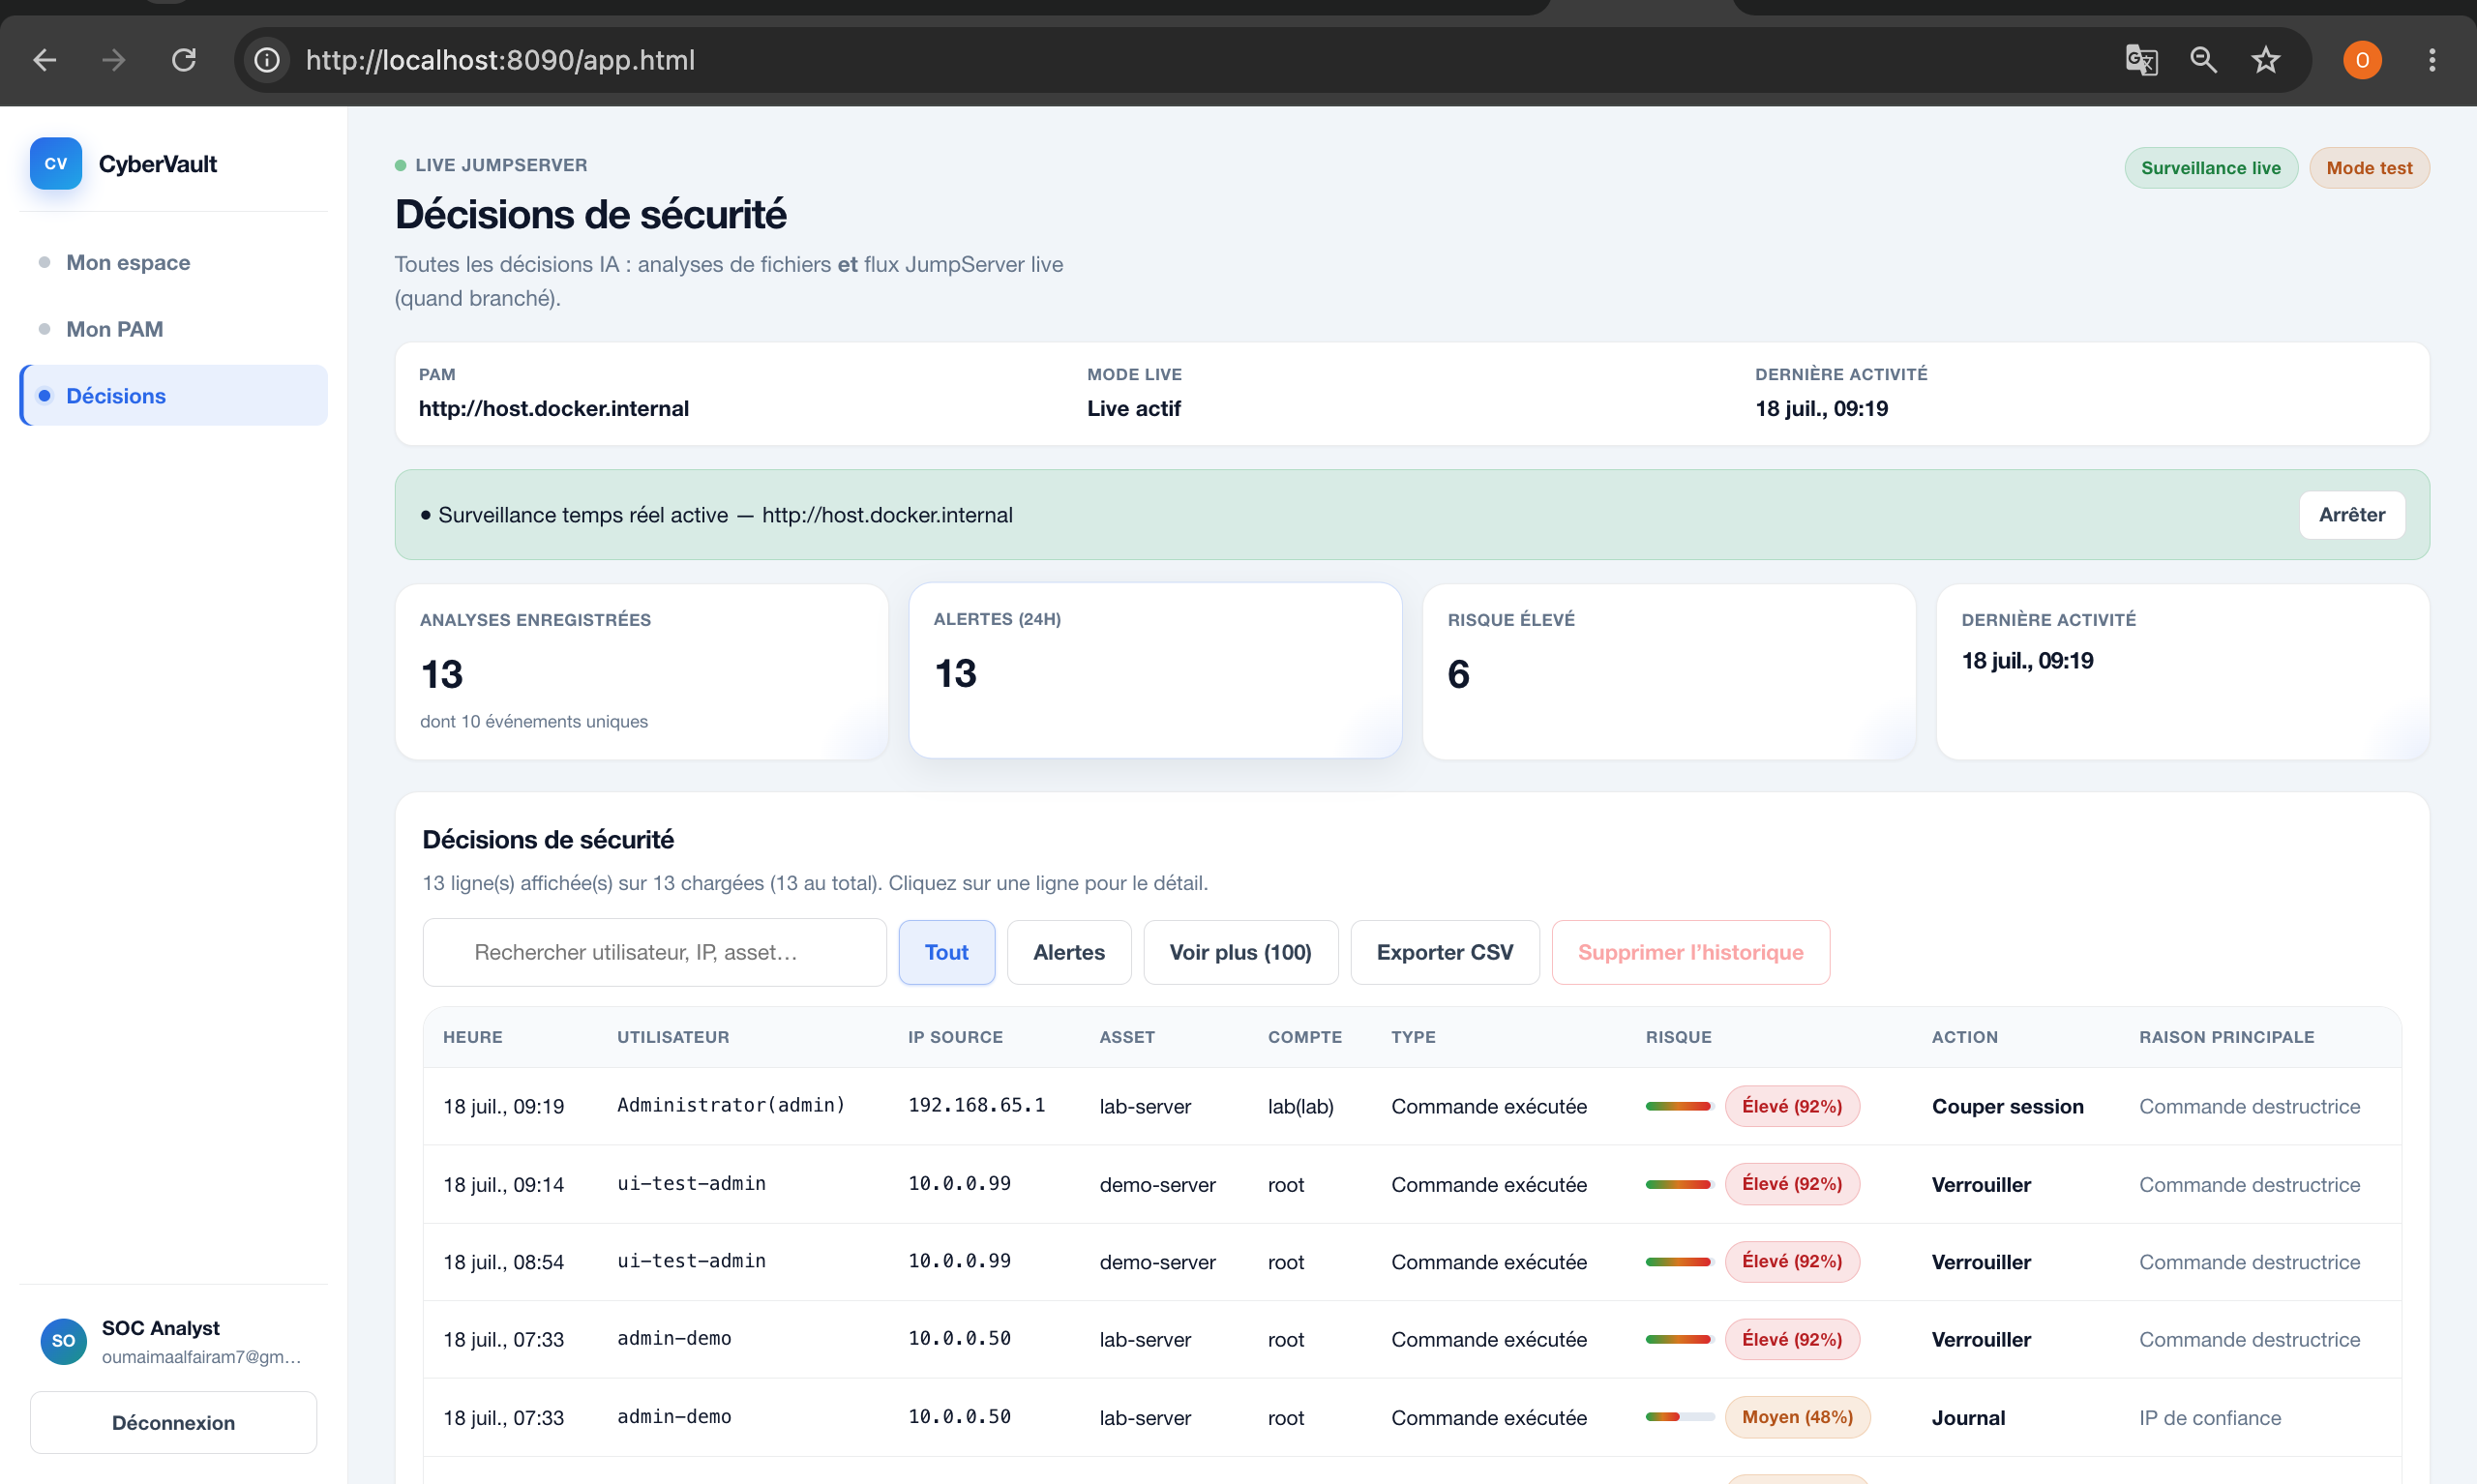
\includegraphics[width=0.92\textwidth]{cybervault-decisions.png}
\caption{Tableau de bord \emph{Décisions de sécurité} : surveillance live,
indicateurs d'alerte et journal des actions (coupure, verrouillage,
journalisation) avec motifs explicites.}
\label{fig:ui-decisions}
\end{figure}

Ce parcours ne prétend pas à une latence nulle. Entre la frappe, l'enregistrement
JumpServer, le transport, l'analyse, l'appel d'API et le rafraîchissement de
l'interface, plusieurs secondes peuvent s'écouler. Il démontre en revanche la
chaîne de bout en bout : observation, décision inspectable, effet sur la
session et, le cas échéant, alerte e-mail.

\section{Algorithme global du traitement en ligne}

Le pseudocode suivant constitue l'unique description algorithmique de bout en
bout. Il rend explicites la dégradation en l'absence d'artefacts, la portée de
l'XAI et la position tardive de l'apprentissage comportemental.

\begin{algorithm}[H]
\caption{Traitement en ligne global d'un événement CyberVault}
\label{alg:method-online}
\begin{algorithmic}[1]
\Require activité JumpServer \(o\), configuration, états persistés, artefacts facultatifs
\Ensure décision journalisée \(d\), état sauvegardé au mieux
\State \(e\leftarrow\Call{BuildEvent}{o}\)
\State \(t\leftarrow\Call{SelectTransport}{configuration}\)
\State \(\Call{CeleryPublishBestEffort}{e,t}\)
\State \(e\leftarrow\Call{Ingest}{fichier,Redis,HTTP}\) \Comment{aucun consommateur Kinesis}
\State \(e_v\leftarrow\Call{DecodePayload}{e}\) \Comment{pas de validation métier formelle}
\State \(\tilde e,\mathbf{x}\leftarrow\Call{EnrichAndFeatures}{e_v,FeatureStore}\)
\State \(R\leftarrow\Call{Rules}{\tilde e}\) ; \(B\leftarrow\Call{UEBAEvaluate}{\tilde e,BaselineStore}\)
\State \(I\leftarrow\Call{IFIfAvailable}{\mathbf{x}}\) ; \(F\leftarrow\Call{RFIfAvailable}{\mathbf{x}}\)
\State \(M\leftarrow\Call{BlendAvailable}{I,F,0.40,0.60}\) \Comment{sinon statut indisponible}
\State \(S\leftarrow\Call{LSTMIfAvailable}{\tilde e}\) ; \(G\leftarrow\Call{GNNIfAvailable}{\tilde e}\)
\State \(r,c,motifs\leftarrow\Call{MaxFusion}{R,B,M,S,G}\)
\If{\(\Call{XAIGate}{M}\) et RF + matrice de fond disponibles}
  \State \(\phi\leftarrow\Call{ExplainRF}{F,\mathbf{x}}\)
\Else
  \State \(\phi\leftarrow\emptyset\)
\EndIf
\State \(\hat a\leftarrow\Call{ThresholdMap}{r}\)
\If{\(\hat a\) est admissible}
  \State \(a^*\leftarrow\hat a\)
\Else
  \State \(a^*\leftarrow\Call{ScalarizedFallback}{r,c,\tilde e}\)
\EndIf
\State \(z\leftarrow\Call{ExecuteJumpServer}{a^*,\tilde e}\) si hors \emph{dry-run}
\State \(d\leftarrow\Call{AppendDecisionLog}{\tilde e,r,c,motifs,\phi,a^*,z}\)
\State \(\Call{NotifyBestEffort}{d}\) si éligible
\If{\(r\leq0.40\)}
  \State \(\Call{UpdateBaseline}{BaselineStore,\tilde e}\)
\EndIf
\State \(\Call{Persist}{FeatureStore,BaselineStore,statuts}\)
\State \(\Call{ExposeToDashboard}{d,statuts}\) \Comment{sans SIEM ni ticketing}
\State \Return \(d\)
\end{algorithmic}
\end{algorithm}

\section{Synthèse et transition vers la validation}

La chaîne temps réel offre une orchestration cohérente et inspectable. Le hook
préserve la sémantique JumpServer ; Celery découple les entrées-sorties ; les
transports rendent l'intégration adaptable ; l'ingestion et le décodage
rendent les entrées traitables ; l'enrichissement fournit le contexte ; règles
et UEBA maintiennent une détection disponible sans poids appris ; IF/RF, puis
LSTM/GNN, interviennent lorsque leurs artefacts existent ; le maximum conserve
le signal sévère ; l'XAI documente RF ; les seuils et le repli produisent une
action admissible ; enfin, journalisation, notification, contrôle conditionnel,
apprentissage filtré et persistance rendent le résultat exploitable.

Cette architecture établit les conditions de validation : événements livrés de
manière asynchrone, producteur Kinesis implémenté, effets contrôlés par le
mode simulation, explication ciblée sur RF et interface locale pour
l'investigation. La section suivante aborde la validation en distinguant
clairement la qualité algorithmique mesurée, la disponibilité de bout en bout
et l'effectivité des actions.



\section{Résultats expérimentaux principaux}

\subsection{Objet de la validation et périmètre probant}
\label{sec:validation-scope}

Cette section met en relation les résultats expérimentaux, les choix de
conception et les conditions d'emploi de CyberVault. Les expérimentations
réalisées couvrent trois plans introduits au chapitre~\ref{chap:impl} :
l'adaptation de corpus publics et de traces de laboratoire (CERT, LANL,
télémétrie JumpServer), les essais techniques de bout en bout (Docker,
intégration bastion, sessions SSH/RDP, réponse et POC AWS), ainsi que la
comparaison des politiques de réponse multi-objectifs. Les résultats des
règles expertes, de l'UEBA, de l'Isolation Forest, de la Random Forest et de
leur fusion sont documentés dans les
Tableaux~\ref{tab:method-rules-results}, \ref{tab:method-ueba-results},
\ref{tab:method-if-results}, \ref{tab:method-rf-results} et
\ref{tab:method-hybrid-results}. Ils constituent le point de départ de
l'analyse transversale des compromis entre méthodes.

Le principal artefact quantitatif agrégé est le fichier
\texttt{ai-security-service/data/research/benchmark\_results.json}. Il décrit
une exécution historique sur 1\,000 événements synthétiques complémentaires et
un pli de test commun aux cinq méthodes. Cette archive conserve graine,
partage et métriques agrégées, établissant ainsi une base auditable pour
l'évaluation. La frontière entre code, configuration et mesure expérimentale
est maintenue explicitement.

Les corpus CERT et LANL, ainsi que la télémétrie JumpServer de laboratoire,
élargissent le périmètre au-delà du générateur : ils documentent
respectivement le transfert de formats hors ligne et le comportement du
pipeline en conditions de session réelle contrôlée. Le jeu synthétique offre
un rôle de non-régression contrôlée : prévalence définie, motifs programmés et
partition documentée permettent une validation méthodologique reproductible.

Le jeu contrôlé vérifie la transformation et la combinaison cohérentes de
signaux hétérogènes. Le pli commun rend visibles les orientations des
détecteurs et fournit un cas de non-régression auditable. Les essais
JumpServer démontrent qu'une décision peut être produite et, hors simulation,
relayée vers une action de session, établissant ainsi la chaîne de bout en
bout.

\begin{table}[H]
\centering
\small
\caption{Couverture réelle des dimensions d'évaluation demandées.}
\label{tab:validation-metric-coverage}
\begin{tabularx}{\textwidth}{@{}p{3.4cm}p{2.2cm}X@{}}
\toprule
\textbf{Dimension} & \textbf{Statut} & \textbf{Justification}\\
\midrule
Exactitude, précision, rappel, $F_1$, FPR & Disponible &
Calculables à partir des cinq matrices agrégées au seuil $0.55$.\\
ROC-AUC et PR-AUC & Indisponible &
Les scores individuels et les points de courbe ne sont pas archivés.\\
Temps de détection et d'inférence & Non mesuré &
Aucun chronométrage brut, percentile, matériel figé ou protocole chaud/froid.\\
Mémoire & Non mesurée &
Aucun pic RSS, taille complète des artefacts ou profil par composant.\\
Coût de calcul & Théorique seulement &
Des complexités asymptotiques sont données, sans benchmark reproductible.\\
Qualité XAI & Non validée &
Exemples techniques disponibles, sans fidélité agrégée ni étude analyste.\\
Qualité de la réponse MOO & Non discriminée &
Le proxy binaire ne conserve pas les actions détaillées ni leurs coûts.\\
\bottomrule
\end{tabularx}
\end{table}


\subsection{Comparaison transversale des compromis de détection}
\label{sec:validation-detection}

La comparaison détaillée du chapitre~\ref{sec:method-ai-ro} ne fait apparaître aucune
méthode dominant toutes les autres. Les règles expertes et la Random Forest
sont les plus sélectives sur le pli archivé : elles limitent fortement les
signalements indus, mais laissent échapper une part importante des anomalies.
L'UEBA étend la couverture en comparant l'activité à des habitudes apprises,
au prix d'alertes supplémentaires. L'Isolation Forest adopte, au point de
fonctionnement conservé, le comportement le plus agressif à l'égard des
événements normaux. La fusion par maximum obtient la meilleure couverture et
le meilleur \(F_1\) archivés, mais hérite de faux positifs produits par ses
composantes. Ce résultat doit être lu comme un déplacement du point de
fonctionnement vers le rappel et non comme une supériorité absolue.

Les règles relient chaque alerte à une condition révisable. Leur précision
apparente porte toutefois sur peu de prédictions positives et sur des scénarios
qui leur sont favorables ; leur faible couverture rappelle qu'elles ne
reconnaissent que les cas anticipés. Elles conviennent aux interdictions nettes
et aux garde-fous, non aux abus sans signature directe.

L'UEBA repère plutôt une rupture avec le passé d'un utilisateur ou d'un actif,
pertinente lorsqu'une commande légitime dans un rôle devient atypique dans un
autre. Il dépend cependant de l'ordre et de la ligne de base : astreinte,
migration ou prestataire peuvent créer une rupture bénigne, tandis qu'un abus
lent peut être normalisé. Son apprentissage doit donc être borné, réversible
et assorti d'une quarantaine.

L'Isolation Forest ne requiert pas d'annotation complète, mais rareté et
nocivité ne coïncident pas. Ses nombreuses fausses alertes excluent un pilotage
direct d'actions perturbatrices ; son score peut alimenter le triage après
étalonnage sur une prévalence réaliste et avec le contexte nécessaire.

La fusion par maximum privilégie la sensibilité : un composant alarmant impose
son signal, ce qui explique son rappel, mais transmet aussi les dérives ou le
mauvais étalonnage du moteur le plus agressif. Faute de prédictions appariées,
les agrégats ne distinguent pas complémentarité réelle, effet de seuil et
recouvrement particulier au pli.

Ce constat conduit à séparer trois usages. Pour une alerte informative, une
orientation vers le rappel peut être acceptable si le regroupement et la
priorisation maintiennent la charge dans un budget défini. Pour une demande de
confirmation humaine, le score peut soutenir l'investigation sans se
substituer au jugement. Pour une action telle qu'un verrouillage ou une
interruption, le même point de fonctionnement est insuffisant : le coût d'un
faux positif devient beaucoup plus élevé, et des preuves supplémentaires ainsi
que des contraintes strictes sont nécessaires. Détection et autorité de
réponse ne doivent donc pas être confondues. Un soupçon élevé justifie
éventuellement un examen ; il ne constitue pas, à lui seul, une preuve
d'intention malveillante.

Le choix dépend d'une fonction de coût absente du benchmark : gravité, taux
d'arrivée, temps de triage, réversibilité et comptes protégés. Le \(F_1\)
résume un compromis binaire mais symétrise des erreurs aux conséquences
différentes. L'hybride est donc le meilleur candidat archivé pour un triage
orienté couverture ; les méthodes sélectives représentent des fonctionnements
plus conservateurs.


\subsection{Politique à seuils, optimisation et mécanisme de repli}
\label{sec:validation-response}

L'expérience de réponse compare une politique à seuils à une politique
combinant optimisation, contraintes et mécanisme de repli. Sur l'indicateur
binaire conservé, les deux politiques produisent les mêmes décisions
d'intervention au seuil archivé. Ce résultat établit que les deux approches
convergent dans cette configuration spécifique.

L'indicateur binaire agrège plusieurs niveaux d'action (alerte, ticket,
verrouillage, interruption) en une seule classe positive. Or la finalité de
l'optimisation est précisément d'arbitrer entre ces niveaux selon le risque
résiduel, la perturbation, la réversibilité, la fatigue opérationnelle et les
contraintes. L'agrégation masque donc la dimension où une différence pourrait
apparaître. Une évaluation complète nécessiterait de conserver l'action
détaillée par événement, les coûts attendus, les contraintes actives et les
violations évitées.

La formalisation multi-objectifs offre une valeur de conception importante.
Elle rend explicites les hypothèses qu'une cascade de seuils peut dissimuler :
poids attribué au risque, coût d'une interruption, priorité des comptes
d'urgence et limites non négociables. Elle fournit ainsi un langage de
gouvernance et un support d'audit pour les arbitrages de sécurité. Les coûts
et contraintes doivent être approuvés par les parties prenantes, testés par
sensibilité et révisés à partir de conséquences observables.

Le mécanisme de repli offre une sûreté architecturale en cas d'information
manquante, d'infaisabilité ou de défaillance. Un repli sûr choisit l'action
appropriée selon la réversibilité, le rayon d'impact et les procédures
d'urgence : journaliser, alerter, demander confirmation ou interrompre. Cette
propriété architecturale est inspectable ; une évaluation avec traces
détaillées quantifierait sa performance opérationnelle.


\subsection{Analyse des erreurs et traitement de l'incertitude}
\label{sec:validation-errors}

Les résultats du chapitre~\ref{sec:method-ai-ro} permettent de comparer les
nombres agrégés de faux positifs et de faux négatifs au niveau des matrices de
confusion. Cette granularité établit les compromis entre méthodes et fournit
une base pour la comparaison. Une analyse approfondie nécessiterait
l'identification des événements concernés pour attribuer les erreurs à un
scénario, un utilisateur, une session ou une période spécifiques.

Les erreurs présentent des portées différentes : manquer une commande
destructive ou un échec de connexion diffère d'alerter ou de verrouiller à tort
pendant une maintenance. La classification binaire permet de comparer les
méthodes ; une analyse opérationnelle conserverait sous-type, gravité, contexte
et action pour modéliser le risque de manière plus fine.

L'archive conserve une graine et un partage documentés. L'estimation
d'incertitude statistique nécessiterait plusieurs graines et partitions pour
fournir variance entre exécutions, intervalles de confiance et tests
d'hypothèse. Les événements d'un même utilisateur ou d'une même session ne sont
pas indépendants, et l'UEBA maintient un état. Une estimation ultérieure
prendrait l'entité ou la session comme unité de rééchantillonnage, et
réserverait une période finale indépendante lorsque l'ordre temporel importe.

Les métriques agrégées établissent les compromis au point de fonctionnement
conservé. Les scores individuels permettraient l'étude de la proximité au seuil,
des courbes précision--rappel, de l'étalonnage et des points de fonctionnement
alternatifs.

Le résultat établi est que, au point de fonctionnement et sur le pli archivés,
la fusion présente le compromis le plus favorable au rappel parmi les méthodes
comparées. Ce constat est réplicable à partir des effectifs conservés ; une
généralisation à d'autres graines, partitions, populations et périodes
nécessiterait des données complémentaires.


\subsection{Reproductibilité et audit des artefacts}
\label{sec:validation-reproducibility}

\begin{table}[tb]
  \centering
  \caption{Audit du résultat historique archivé.}
  \label{tab:eval-repro-audit}
  \small
  \begin{tabular}{@{}p{0.31\linewidth}p{0.18\linewidth}p{0.43\linewidth}@{}}
    \toprule
    Élément & Statut & Conséquence \\
    \midrule
    JSON agrégé & Disponible &
    Effectifs et métriques arrondies auditables \\
    Code du benchmark et des métriques & Disponible &
    Logique actuelle inspectable \\
    Graine et partition & Documentées &
    Graine et partage historiques connus \\
    Entrée historique à 1\,000 événements & Archive distincte &
    Générateur évolué vers 1\,640 événements enrichis \\
    Scores, actions et modèles entraînés & Niveau agrégé conservé &
    Métriques au niveau de confusion disponibles \\
    Environnement et matériel & Documenté au niveau configuration &
    Environnement logiciel versionné \\
    \bottomrule
  \end{tabular}
\end{table}

L'audit du Tableau~\ref{tab:eval-repro-audit} établit la distinction entre
auditabilité et reproductibilité complète. Le JSON permet de recalculer les
indicateurs agrégés et de vérifier la cohérence arithmétique des effectifs. Le
code actuel permet d'inspecter la logique générale. Ces éléments rendent le
résultat historique auditable au niveau de son résumé.

Le générateur a évolué de 1\,000 à 1\,640 événements en intégrant des sessions
progressives, des séquences multicommandes bénignes et des négatifs difficiles
: cette évolution enrichit les capacités de test. Le projet distingue
clairement l'archive historique de 1\,000 événements comme référence
documentée, et le générateur actuel de 1\,640 événements comme outil de
non-régression enrichi. Cette séparation méthodologique préserve la traçabilité
des expériences passées tout en offrant des capacités étendues pour les
validations futures.

L'architecture actuelle fournit une base pour l'extension : un paquet complet
associerait données et empreintes, code, configuration, dépendances,
partitions, schéma de caractéristiques, modèles, scores, prédictions, actions
et mesures brutes. L'archive actuelle permet la vérification du résumé
quantitatif.

Le projet établit plusieurs garde-fous méthodologiques : vérification des
effectifs, séparation explicite des étiquettes et des caractéristiques,
documentation de l'ordre des événements et distinction entre divergences
tolérées et écarts invalidants. Cette discipline méthodologique offre une base
pour la gouvernance des modèles en production, où la traçabilité des versions
et des politiques est essentielle.



\chapter{Analyse et discussion}
\label{chap:discussion}

Ce chapitre évalue les réalisations du prototype CyberVault, répond aux questions de recherche et examine les conditions d'adoption industrielle. Il rassemble ensuite les limites scientifiques et opérationnelles ainsi que les perspectives prioritaires dans une section unifiée. Les mesures détaillées ont été présentées au Chapitre~\ref{chap:impl} ; l'accent est placé ici sur l'interprétation constructive des contributions et sur la définition d'une progression rigoureuse vers un éventuel déploiement opérationnel.

\section{Synthèse des résultats expérimentaux}
\label{sec:discussion-results}

Les expérimentations menées établissent plusieurs réalisations architecturales, techniques et métriques. Le prototype CyberVault fonctionne de bout en bout : instrumentation réussie de JumpServer, ingestion multi-canal opérationnelle (fichier, Redis, HTTP, Kinesis), traitement analytique hybride combinant règles, UEBA et apprentissage automatique, génération d'explications SHAP et LIME, et simulation de réponses graduées sous contraintes. Les adaptateurs développés pour les corpus publics CERT Insider Threat et LANL permettent l'ingestion et le traitement de données de référence, démontrant la capacité du système à s'intégrer avec des sources standardisées. Les validations techniques couvrent le déploiement Docker, l'intégration SSH et RDP avec JumpServer, et une preuve de concept AWS EC2.

Sur le plan métrique, le benchmark synthétique historique de 300 événements fournit une base de comparaison descriptive entre détecteurs. La fusion hybride atteint un score $F_1$ de $66{,}23\%$ et un rappel de $81{,}97\%$, représentant le meilleur compromis archivé dans cette configuration et démontrant l'intérêt de combiner plusieurs familles de détection. Une expérimentation bornée sur les politiques de réponse multi-objectifs complète ce volet, établissant la faisabilité de l'optimisation sous contraintes même si la supériorité métrique par rapport aux seuils fixes reste à démontrer sur l'espace complet des actions.

Ces éléments établissent la faisabilité de l'architecture proposée et fournissent une base inspectable pour un pilote en simulation. Les sections suivantes répondent aux questions de recherche, précisent les implications industrielles, puis rassemblent les limites scientifiques et les perspectives dans une section unifiée qui définit les validations complémentaires nécessaires à un déploiement opérationnel.


\section{Réponses aux questions de recherche}
\label{sec:validation-rqs}

Les quatre sous-questions et la question principale de recherche sont examinées à la lumière des éléments probants disponibles.

\paragraph{SRQ1 : détection hybride.}
La fusion par maximum des scores de règles, UEBA et modèles tabulaires atteint le meilleur rappel et le meilleur \(F_1\) archivés sur le pli synthétique au seuil de \(0.55\), démontrant l'intérêt d'une approche hybride pour privilégier la couverture. Ce résultat établit la valeur de la combinaison dans le cadre expérimental étudié. Les validations complémentaires nécessaires en matière de stabilité statistique, d'étalonnage et de transfert à d'autres sources sont précisées en section~\ref{sec:limites-perspectives}.

\paragraph{SRQ2 : caractère exploitable des explications.}
Le système génère avec succès des explications SHAP et LIME ainsi que des justifications textuelles issues des règles et du profilage comportemental. Ces capacités d'explication sont opérationnelles et inspectables, constituant une base technique solide. L'évaluation de leur utilité opérationnelle pour les analystes --- impact sur l'exactitude, le temps de décision et le biais d'automatisation --- constitue une perspective prioritaire détaillée en section~\ref{sec:limites-perspectives}.

\paragraph{SRQ3 : optimisation de la réponse.}
L'architecture de décision sous contraintes est formalisée, implémentée et inspectable. La comparaison bornée des politiques de réponse (optimisation multi-objectifs vs seuils) a été menée selon un indicateur binaire, configuration dans laquelle les deux approches obtiennent des résultats équivalents. L'évaluation complète nécessite des métriques distinguant les coûts, réversibilités, contraintes et préjudices de chaque niveau d'action (alerte, ticket, verrouillage, interruption), dimension détaillée en section~\ref{sec:limites-perspectives}.

\paragraph{SRQ4 : valeur de l'intégration.}
L'intégration de la chaîne détection--explication--décision accroît la sensibilité mesurée et démontre la faisabilité de l'architecture complète tout en conservant la provenance des signaux et en séparant le calcul du risque de l'autorité d'action. Le prototype établit la traçabilité des décisions et la modularité de l'approche. Les ablations contrôlées isolant la contribution causale de chaque composante, l'évaluation de la XAI avec des analystes et la différenciation entre politiques de réponse constituent des extensions prioritaires précisées en section~\ref{sec:limites-perspectives}.

\begin{table}[tb]
  \centering
  \caption{Réponses aux questions de recherche selon les preuves disponibles.}
  \label{tab:disc-rq-summary}
  \small
  \begin{tabular}{@{}p{0.11\linewidth}p{0.25\linewidth}p{0.54\linewidth}@{}}
    \toprule
    Question & État & Conclusion \\
    \midrule
    SRQ1 & Démontrée sur benchmark archivé &
      La fusion hybride atteint le meilleur rappel et \(F_1\) archivés, démontrant l'intérêt de combiner règles, UEBA et apprentissage. Validation externe et stabilité statistique à établir. \\
    SRQ2 & Capacité technique établie &
      Les explications SHAP/LIME et justifications textuelles sont fonctionnelles et inspectables. Évaluation de l'utilité opérationnelle avec analystes à mener. \\
    SRQ3 & Architecture formalisée &
      L'architecture de décision sous contraintes est opérationnelle et inspectable. Évaluation comparative sur actions différenciées à compléter. \\
    SRQ4 & Architecture validée, contributions à isoler &
      L'intégration apporte une valeur mesurable en sensibilité et traçabilité. Ablations contrôlées à réaliser pour isoler la contribution causale de chaque maillon. \\
    MRQ & Étayée en laboratoire &
      CyberVault fournit une chaîne inspectable pour le triage et la validation
      technique en environnement contrôlé. Les validations opérationnelles
      complémentaires sont définies en section~\ref{sec:limites-perspectives}. \\
    \bottomrule
  \end{tabular}
\end{table}

La réponse à la question principale de recherche (MRQ) confirme que CyberVault fournit une combinaison inspectable et fonctionnelle de règles, UEBA, apprentissage tabulaire, explications et décision sous contraintes pour soutenir l'analyse des événements PAM. Le prototype atteint les objectifs architecturaux, démontre la faisabilité de l'intégration complète et établit des éléments de comparaison descriptive en laboratoire. Les validations opérationnelles complémentaires nécessaires à un déploiement en production sont précisées en section~\ref{sec:limites-perspectives}. Le Tableau~\ref{tab:disc-rq-summary} synthétise cette lecture équilibrée des preuves disponibles.


\section{Implications industrielles et conditions d'adoption}
\label{sec:validation-industry}

Le prototype CyberVault offre plusieurs voies d'exploitation industrielle graduées selon le niveau de risque acceptable. À court terme, le rôle le plus approprié est celui d'un pilote en mode \emph{dry-run}, adjacent au dispositif PAM existant. Dans cette configuration, CyberVault reçoit une copie des événements, calcule ses scores, génère des explications et journalise les actions qu'il aurait proposées, sans modifier l'état des sessions actives. Cette approche permet de mesurer la charge d'alertes, d'identifier les cas récurrents, de corréler les signaux avec les incidents connus et de réviser progressivement les politiques, tout en préservant la continuité opérationnelle.

Le prototype complète, sans remplacer, les contrôles PAM existants : authentification, habilitations, enregistrement et procédures d'urgence conservent leur autorité. L'architecture hybride démontre la faisabilité d'une détection enrichie et la traçabilité des décisions. Une adoption progressive doit toutefois s'appuyer sur des critères mesurables : budget acceptable de faux positifs, charge d'investigation, objectifs de détection adaptés à la prévalence réelle et aux conséquences des actions.

Le suivi en exploitation devrait couvrir la dérive des modèles, la disponibilité des données, la gestion des dérogations et le retour d'expérience sur les actions proposées. Chaque recommandation devrait porter les versions du modèle, de la politique et du schéma d'événements afin d'assurer la reproductibilité et l'audit. Les lignes de base comportementales nécessitent un apprentissage borné et un mécanisme de retour arrière pour éviter qu'une activité hostile progressive ne devienne progressivement considérée comme normale.

L'adoption doit rester proportionnée à la réversibilité des actions. Une alerte ou un ticket peut tolérer un niveau d'incertitude supérieur à un verrouillage. Les actions perturbatrices exigent une approbation humaine, un double contrôle pour les ressources critiques, une durée bornée et une procédure de restauration testée. Les comptes d'urgence, les opérations de reprise et les fenêtres de maintenance doivent bénéficier de protections explicites. La fonction analytique ne doit jamais devenir un point unique capable de provoquer un déni de service sur le plan de contrôle.


\section{Éthique, responsabilité et sûreté}
\label{sec:validation-ethics}

Les conséquences d'une erreur dépendent moins de son étiquette binaire que de
l'action qui la suit. Une fausse alerte consomme du temps ; un verrouillage
injustifié peut interrompre une maintenance, empêcher une reprise ou affecter
un service essentiel. L'automatisation doit donc exiger davantage de preuves
que le triage et appliquer les principes de moindre privilège, de
réversibilité, de limitation du rayon d'impact et de séparation des fonctions.
Une responsabilité explicite doit être attribuée pour la validation des
politiques, les dérogations et l'examen après incident.

Les explications enrichissent le triage lorsqu'elles sont présentées comme
des descriptions locales du modèle, accompagnées des données manquantes, de la
version, des facteurs contradictoires et d'un degré d'incertitude. L'interface
autorise l'analyste à confirmer ou contester la recommandation ; les désaccords
sont enregistrés comme des informations de gouvernance.

La télémétrie privilégiée révèle des habitudes de travail, des horaires, des
lieux, des actifs sensibles et parfois le contenu d'opérations. Les principes
de minimisation, de limitation des finalités et de la conservation, de
chiffrement et d'accès auditable s'appliquent même après pseudonymisation. Les
compromis entre confidentialité et utilité analytique, ainsi que les
transformations envisagées, sont détaillés au chapitre~\ref{chap:impl}. Dans la
validation, il importe surtout de ne pas confondre absence d'identifiant direct
et absence de risque de réidentification.

Travail distant, astreintes et urgences peuvent produire davantage d'écarts.
Le suivi par groupes légitimes, ainsi que les recours et corrections, doivent
empêcher qu'une pratique différente devienne une suspicion personnelle.

Enfin, le système lui-même appartient au modèle de menace. Un attaquant peut
éviter les signatures, étaler son activité, provoquer des alertes ou empoisonner
les lignes de base. Un service analytique compromis pourrait devenir un outil
de déni de service s'il contrôle des interruptions. Des journaux protégés
contre l'altération, une limitation de débit, une supervision indépendante et
un comportement sûr en cas de panne sont indispensables. La sûreté ne résulte
pas de la seule précision d'un classifieur ; elle dépend de la gouvernance de
toute la chaîne de décision.


\section{Déploiement progressif et adoption industrielle}
\label{sec:validation-roadmap}

Le prototype CyberVault offre plusieurs voies d'exploitation industrielle graduées selon le niveau de maturité des validations. La trajectoire recommandée privilégie l'observation et l'apprentissage organisationnel avant toute automatisation d'actions perturbatrices.

\paragraph{Phase pilote en mode observation.} À court terme, le rôle le plus approprié est celui d'un pilote en mode \emph{dry-run}, adjacent au dispositif PAM existant et sans autorité d'action. Dans cette configuration, CyberVault reçoit une copie des événements, calcule ses scores, génère des explications et journalise les actions qu'il aurait proposées, sans modifier l'état des sessions actives. Cette approche permet de mesurer la charge d'alertes, d'identifier les faux positifs récurrents, de calibrer les seuils et politiques, de corréler les signaux avec les incidents connus et d'évaluer la pertinence des explications pour les analystes, tout en préservant la continuité opérationnelle.

\paragraph{Intégration progressive avec contrôle humain.} Une fois le pilote stabilisé et les politiques affinées sur plusieurs mois de télémétrie, les étapes suivantes peuvent être envisagées : simulation visible permettant aux analystes de commenter et d'enrichir les décisions, puis actions réversibles (verrouillage temporaire, suspension) approuvées manuellement pour les comptes non critiques. Chaque niveau d'automatisation accrue doit être justifié par des critères de sortie mesurables : taux de faux positifs accepté, temps de réponse des analystes, absence de blocages d'opérations légitimes critiques et validation des mécanismes de reprise. Les comptes d'urgence, les opérations de maintenance planifiée et les fenêtres de déploiement doivent bénéficier de protections explicites et testées.

\paragraph{Critères d'adoption et gouvernance.} L'adoption industrielle doit s'appuyer sur une gouvernance explicite couvrant la validation des politiques, la gestion des dérogations, l'audit des actions proposées ou exécutées, et le retour d'expérience systématique sur les incidents. Chaque recommandation devrait porter les versions du modèle, de la politique et du schéma d'événements afin d'assurer la reproductibilité. Le suivi en exploitation doit inclure la dérive des modèles, la disponibilité des données, la latence sous charge réelle et la satisfaction des analystes. Une automatisation complète sans approbation humaine ne devrait être envisagée que pour les actions à faible impact (alertes, tickets) et après validation approfondie selon les critères détaillés en section~\ref{sec:limites-perspectives}.


\section{Limites et perspectives}
\label{sec:limites-perspectives}

Cette section regroupe les limites réellement structurantes du travail et les perspectives qui en découlent. Elle évite de répéter ces points dans le reste du mémoire, afin de laisser place à la présentation des réalisations.

\subsection{Limites scientifiques}

Le benchmark métrique archivé repose sur un pli synthétique unique ($n=300$, seuil $0.55$, graine documentée). Il fournit une comparaison descriptive solide entre détecteurs, mais n'établit pas encore la stabilité multi-graines, l'étalonnage probabiliste ni une généralisation à une prévalence industrielle. CERT Insider Threat et LANL ont été adaptés et exercés pour l'ingestion ; une campagne $F_1$ versionnée, comparable au benchmark PAM, reste à constituer. La proximité sémantique entre certains scénarios générés et les caractéristiques favorise la récupération de motifs programmés : ce choix est utile pour la non-régression, et invite à des validations sur télémétrie annotée indépendante.

Sur le plan décisionnel, la comparaison bornée des politiques (seuils vs repli multi-objectifs) montre l'équivalence selon un proxy binaire ; elle n'évalue pas encore distinctement coûts, réversibilité et préjudice de chaque action. Les explications SHAP/LIME sont opérationnelles et inspectables ; leur utilité pour les analystes (exactitude, temps, biais d'automatisation) n'a pas fait l'objet d'une étude contrôlée. Enfin, aucune campagne de latence sous charge n'est archivée : la faisabilité temps réel est démontrée en laboratoire, sans borne de performance industrialisée.

\subsection{Limites opérationnelles}

CyberVault est un prototype adjacent à JumpServer, conçu pour un déploiement progressif. Le mode simulation par défaut, la séparation entre score et autorité d'action, et la protection des comptes critiques constituent des choix de sûreté. L'industrialisation (haute disponibilité, multi-région, chaîne managée complète, intégration SIEM/ticketing généralisée) dépasse le périmètre du POC, même si Docker, l'intégration bastion et le chemin AWS EC2 en établissent la portabilité.

\subsection{Perspectives prioritaires}

Les perspectives s'organisent autour de six axes, dans la continuité des acquis :
\begin{enumerate}[leftmargin=*]
  \item constituer un corpus expérimental immuable et versionné (empreintes, partitions, modèles, scores individuels) ;
  \item répéter les mesures (graines, séparations par utilisateur, session et période) et publier des intervalles de confiance ;
  \item conduire une campagne métrique sur CERT, LANL puis sur une télémétrie JumpServer approuvée et anonymisée ;
  \item évaluer les politiques de réponse sur l'espace complet des actions (coûts, contraintes, préjudices) ;
  \item mesurer latence à chaud/à froid et utilité des explications avec des analystes ;
  \item progresser par critères de sortie : observation, simulation visible, actions réversibles approuvées, automatisation bornée.
\end{enumerate}

Ces perspectives prolongent CyberVault comme banc d'essai inspectable et comme base d'un pilote opérationnel maîtrisé, plutôt que comme une rupture brutale vers l'autonomie.


\section{Synthèse de la discussion}

CyberVault établit la faisabilité d'une architecture hybride intégrant règles, UEBA, apprentissage tabulaire, explications et décision sous contraintes pour l'analyse des sessions privilégiées. Sur le benchmark synthétique archivé, la fusion démontre un compromis favorable au rappel avec un \(F_1\) de $66{,}23\%$ et un rappel de $81{,}97\%$. L'implémentation complète valide l'instrumentation de JumpServer, les transports multi-canaux, le traitement analytique et la simulation de réponses graduées. Les adaptateurs CERT et LANL ainsi que les validations techniques (Docker, SSH/RDP, AWS) démontrent la capacité d'intégration du système.

Les perspectives prioritaires consolidant ces acquis sont détaillées en section~\ref{sec:limites-perspectives}.

La contribution de CyberVault réside dans l'intégration traçable des mécanismes, dans la séparation entre détection et autorité d'action, dans la formalisation des contraintes de sûreté et dans la définition d'une progression rigoureuse vers un éventuel usage industriel. Le prototype fournit un banc d'essai inspectable pour les politiques de détection et de réponse, ainsi qu'une base solide pour les validations opérationnelles futures. La conclusion générale reprend ces acquis et situe la portée finale de la contribution.


\chapter{Conclusion générale}
\label{chap:conclusion}

Ce mémoire a conçu, implémenté et évalué CyberVault, une couche analytique opérationnelle intégrée à JumpServer pour détecter, expliquer et encadrer la réponse aux comportements suspects observés après l'authentification d'une session privilégiée. La contribution repose sur une chaîne de décision ouverte, traçable et vérifiable qui associe des règles nommées, des lignes de base UEBA, plusieurs modèles d'apprentissage tabulaire, des mécanismes d'explication et une sélection de réponse soumise à des contraintes explicites. Le prototype sépare le calcul du risque de l'autorisation d'agir, conserve la provenance des signaux et privilégie la simulation, permettant d'étudier l'IA appliquée au PAM sans confondre capacité logicielle, performance expérimentale et aptitude au déploiement. L'audit de bout en bout établit ce qui est effectivement implémenté, ce qui demeure expérimental et ce qui relève d'une extension future.

L'architecture réalisée organise CyberVault comme un plan analytique adjacent au plan de contrôle de JumpServer. Les événements de session alimentent des détecteurs complémentaires dont les sorties sont fusionnées et accompagnées d'éléments explicatifs avant qu'une politique ne propose une action graduée. La fusion par maximum traduit un choix volontairement orienté vers la sensibilité, tandis que SHAP et LIME fournissent une capacité d'explication locale fonctionnelle. En aval, la politique sous contraintes distingue l'alerte, l'ouverture d'un ticket, le verrouillage et l'interruption. Cette organisation complète les contrôles PAM existants (identité, habilitations, enregistrement, procédures d'urgence) en ajoutant un niveau d'observation et d'aide à la décision. Sa valeur tient à la modularité, à la traçabilité des propositions et aux contraintes de sûreté qui limitent les effets.

Les résultats expérimentaux établissent plusieurs réalisations mesurables. Sur le sous-ensemble synthétique historique de 300 événements (seuil \(0.55\)), le détecteur hybride atteint un rappel de $81{,}97\%$ et un \(F_1\) de $66{,}23\%$, les meilleurs niveaux archivés dans cette configuration. Par rapport aux règles seules, le \(F_1\) progresse d'environ 15 points et les faux négatifs diminuent de 40 à 11, ce qui met en évidence l'intérêt d'une approche hybride pour privilégier la couverture. Le travail expérimental inclut également l'adaptation de corpus publics de référence (CERT Insider Threat, LANL), la validation opérationnelle du pipeline JumpServer--CyberVault (déploiement Docker, intégration SSH/RDP, preuve de concept AWS EC2), et une comparaison des politiques de réponse. Ces éléments constituent une base solide pour un pilote en simulation, sous contrôle explicite du coût des alertes et de la gravité des actions.

Les limites scientifiques et opérationnelles, ainsi que les perspectives prioritaires, sont rassemblées en section~\ref{sec:limites-perspectives}. CyberVault s'y présente comme un prototype de recherche inspectable et un banc d'essai de politiques, prêt à soutenir une progression graduée vers un usage industriel.

CyberVault établit ainsi un socle auditable pour étudier comment une détection comportementale hybride peut soutenir l'analyse des sessions privilégiées tout en préservant la maîtrise humaine des opérations critiques. La contribution scientifique réside dans l'intégration traçable des mécanismes de détection et d'explicabilité, dans la formalisation des contraintes d'action et de sûreté, et dans la définition d'une trajectoire méthodique vers un éventuel usage industriel. Le prototype démontre la faisabilité architecturale d'une approche IA--recherche opérationnelle pour la surveillance comportementale des accès privilégiés, et ouvre la voie à des validations opérationnelles qui pourront confirmer et affiner cette proposition.

\appendix

\chapter{Annexe : éléments de pilotage}
\label{chap:app-management}

Cette annexe rappelle brièvement que le projet a été suivi avec une approche Agile/Kanban adaptée à un POC. Les registres détaillés de backlog, user stories et risques ont servi à l'organisation du stage, mais ne constituent pas le cœur scientifique du mémoire. Les figures de planification éventuellement conservées dans le dépôt documentaire peuvent être consultées séparément si nécessaire.

\section{Une conduite adaptée à une preuve de concept exploratoire}

CyberVault relève à la fois de la recherche appliquée et de l'ingénierie : il
fallait comprendre la télémétrie de JumpServer, éprouver plusieurs familles de
détection, formuler une décision sous contraintes, puis construire un protocole
d'évaluation et en expliciter les limites. Dans un tel contexte, l'incertitude
ne porte pas seulement sur la charge de travail, mais aussi sur la pertinence
des pistes techniques. Une hypothèse peut être abandonnée après une expérience,
une interface peut évoluer lorsque le schéma d'événements est mieux compris et
un résultat intermédiaire peut modifier la priorité du travail suivant.

L'\emph{Agile} est ici compris comme un ensemble de principes de pilotage
favorisant l'adaptation, la livraison incrémentale et le retour fréquent sur un
résultat observable. Le terme ne désigne donc ni l'absence de planification ni
l'application automatique d'un cadre particulier. La planification reste
nécessaire, mais elle est révisable à mesure que les connaissances progressent.
Pour ce POC, un flux Kanban continu a été préféré à Scrum. Kanban rend visible
l'état des éléments de travail, limite l'encours et autorise le réordonnancement
du travail restant sans attendre la frontière d'une itération. Cette souplesse
est cohérente avec un projet individuel, exploratoire, dans lequel les activités
de lecture, d'intégration, d'expérimentation et de rédaction s'entrecroisent.

Scrum aurait exigé de documenter des rôles, un objectif de sprint, un
engagement de contenu, des événements récurrents et un incrément évalué à chaque
itération. Le projet a privilégié, de façon délibérée, des
\textbf{cycles hebdomadaires de planification} : examen des travaux
terminés, actualisation des risques, choix du prochain élément admissible et
vérification de la capacité disponible. Une revue plus large pouvait être
menée avec l'encadrement, dans un rythme adapté au POC plutôt qu'à un cadre
Scrum formalisé.

\chapter{Annexe : Dossier de reproductibilité}
\label{app:reproducibility}

Cette annexe délimite ce qui peut être vérifié et ce qui peut être régénéré.
L'artefact numérique faisant autorité est
\path{ai-security-service/data/research/benchmark_results.json} ; le fichier
\path{BENCHMARK_REPORT.md} adjacent en donne une présentation arrondie. Aucune
prédiction par événement, aucun modèle ajusté, aucune trace temporelle et aucun
verrouillage complet de l'environnement n'accompagnent cette exécution. Le
répertoire audité n'étant pas une copie de travail Git, aucun commit ne peut
être attribué au résultat. Ces absences appartiennent au manifeste : elles ne
doivent pas être reconstituées a posteriori.

\section{Manifeste}
\label{app:manifest}

\begin{table}[H]
\centering
\caption{Manifeste du benchmark CyberVault archivé.}
\label{tab:app-manifest}
\small
\begin{tabular}{@{}p{0.25\textwidth}p{0.67\textwidth}@{}}
\toprule
Élément & Valeur auditée \\
\midrule
Expérience & Classification binaire d'événements privilégiés synthétiques ;
graine 42 ; mélange puis partition positionnelle 70/30 ; seuil 0.55. \\
Population & 1\,000 événements, dont 800 normaux et 200 anormaux ; les
anomalies déclarées couvrent commandes destructrices, heures, actifs et IP
inhabituels, combinaisons latérales et échecs de connexion. \\
Test & 300 événements : 239 négatifs et 61 positifs, d'après les effectifs
archivés présentés dans les tables de la méthode et de l'évaluation. \\
Méthodes & Règles, UEBA, Isolation Forest, Random Forest et hybride par maximum. \\
Résultats & \path{ai-security-service/data/research/benchmark_results.json}\\
& SHA-256 :
\nolinkurl{9b7988e83293b5be87d3eab74829d3ea7cf5de045e48f2e72d78a8441cc290c1}. \\
Rapport & \path{ai-security-service/data/research/BENCHMARK_REPORT.md}\\
& SHA-256 :
\nolinkurl{d4fc9fd1a4519cf688fe14531bc79c540fd29ac2d39d32c73337557c8665a355}. \\
Dépendances & \path{ai-security-service/requirements.txt}\\
& SHA-256 :
\nolinkurl{82cf4b6dd2bd748cbd5e49aad5f046be5a6735b8732155aa94e17f26db3da863};
plages de versions, sans environnement entièrement résolu. \\
Logiciels déclarés & Python 3.10 ou ultérieur, Redis, Requests, PyYAML, NumPy
\((\geq1.24,<2)\), scikit-learn \((\geq1.3)\), SHAP, LIME et PyTorch. \\
Commande & Depuis \path{ai-security-service/} :
\texttt{python -m aiss.evaluation.run\_benchmark --output data/research --seed 42}. \\
\bottomrule
\end{tabular}
\end{table}

\section{Procédure de vérification et limites}

Une vérification minimale consiste à recalculer les trois empreintes SHA-256,
à contrôler qu'elles correspondent au tableau~\ref{tab:app-manifest}, puis à
comparer les métriques du JSON au rapport mis en forme. Les effectifs détaillés
ne sont pas reproduits ici afin d'éviter une matrice dupliquée ; ils restent
dans les tables de la méthode et du chapitre d'évaluation, auxquelles la
discussion se réfère. Le contrôle doit également confirmer la graine, le seuil,
la taille du test et l'identité des méthodes avant toute comparaison.

Pour une nouvelle exécution, le dossier devrait recevoir un identifiant unique
et un manifeste généré automatiquement. Celui-ci associerait les empreintes des
données, de la configuration, du code, de l'image d'exécution et des sorties.
Les journaux indiqueraient la plateforme, les graines de chaque bibliothèque et
les avertissements d'entraînement. Les résultats ne seraient promus vers le
rapport qu'après vérification de ces liens et des sommes de population. Cette
chaîne de garde rendrait détectable toute substitution silencieuse d'un fichier
ou d'une politique.

La commande indiquée produit un nouveau benchmark, mais ne recrée pas
exactement l'artefact historique. Le générateur actuel audité émet 1\,640
événements, alors que le résultat conservé en décrit 1\,000. Les métadonnées des
modèles existent, mais les poids pickle, NumPy et PyTorch requis par les
chargeurs ne sont pas versionnés. Les versions déclarées des bibliothèques ne
suffisent pas non plus à reconstruire exactement les dépendances transitives,
la plateforme et les variantes numériques utilisées.

Une réexécution strictement reproductible exigerait donc une copie immuable du
générateur historique, les événements produits ou leurs indices de partition,
un environnement résolu avec image de conteneur, les modèles ajustés et les
scores de chaque composant par événement. Elle devrait en outre conserver les
versions de la politique, les explications, les actions proposées et les
mesures temporelles brutes. En leur absence, le JSON doit être cité comme une
mesure historique archivée, et toute nouvelle exécution comme une expérience
distincte. Cette convention évite d'attribuer à une régénération actuelle la
provenance ou les garanties de l'artefact initial. Elle permettrait aussi de
recalculer de nouvelles métriques sans réentraîner les modèles et d'étudier les
erreurs appariées, ce que les seuls agrégats actuels interdisent.

% Label historique conservé pour les renvois existants ; la matrice dupliquée
% a été remplacée par un renvoi aux tables de la méthode et de l'évaluation.
\phantomsection
\label{app:confusion-counts}
\label{tab:app-confusion}

\chapter{Annexe : Périmètre de l'état d'implémentation}
\label{app:status}

Le tableau~\ref{tab:app-status} résume l'état d'implémentation observé dans le
dépôt : fonctions opérationnelles, capacités partielles et extensions prévues.

\begin{longtable}{@{}p{0.27\textwidth}p{0.18\textwidth}p{0.47\textwidth}@{}}
\caption{État compact des fonctionnalités CyberVault.}
\label{tab:app-status}\\
\toprule
Fonctionnalité & État & Portée probante \\
\midrule
\endfirsthead
\toprule
Fonctionnalité & État & Portée probante \\
\midrule
\endhead
Événements JumpServer ; transports fichier, Redis et HTTP &
Implémentés & Hooks, producteurs et voies d'ingestion opérationnels (livraison
asynchrone au mieux). \\
Règles et UEBA & Implémentées & Motifs déterministes et lignes de base avec
état exécutables dans la notation en direct. \\
Isolation Forest--Random Forest & Implémenté, artefacts incomplets & Code
d'entraînement et d'inférence présent ; poids absents de l'extraction, donc un
nouveau service peut être non entraîné. \\
Fusion par maximum et réponse MOO & Implémentées & Décisions et contraintes
journalisées ; verrouillage et interruption disponibles, avec simulation par
défaut. \\
SHAP/LIME & Implémentés & Explicateurs conditionnels opérationnels ; étude
d'utilité auprès d'analystes prévue (voir limites). \\
Tableau de bord et JSON/JSONL & Preuve de concept & Vues et persistance locale
opérationnelles pour le POC. \\
LSTM, Transformer et GNN & Expérimentaux & Interfaces et entraînement présents,
mais poids absents et modèles exclus du benchmark tabulaire archivé. \\
MOO des privilèges & Consultative & Recommandation journalisée, prête à être
reliée à un actionneur d'ACL audité. \\
Kinesis & Partielle & Producteur présent, sans consommateur ni point de reprise. \\
Tickets et export SIEM & Prévus & Ticket différé ; export non industrialisé. \\
Validation CERT/LANL & Adaptée & Chargeurs, notebook et essais d'ingestion ;
campagne $F_1$ versionnée en perspective. \\
Plateforme cloud & POC & Preuve de concept CloudFormation/EC2 ; industrialisation
multi-AZ et SLA en feuille de route. \\
\bottomrule
\end{longtable}

\chapter{Annexe : Éthique et IA responsable}
\label{app:ethics}

Cette checklist complète la discussion de la
section~\ref{sec:validation-ethics} sans en répéter l'analyse. Elle doit être
réexaminée avant chaque changement de données, de modèle, de politique ou de
niveau d'automatisation.

\begin{itemize}[leftmargin=*]
  \item \textbf{Finalité et proportionnalité :} documenter l'objectif de
  sécurité, exclure les usages disciplinaires automatiques et vérifier que la
  collecte reste proportionnée au risque.

  \item \textbf{Données :} minimiser commandes, identifiants, actifs, adresses
  et horodatages ; définir conservation et suppression ; chiffrer les données
  et limiter les accès selon les rôles.

  \item \textbf{Vie privée :} pseudonymiser les jeux d'évaluation, évaluer le
  risque de réidentification par actifs rares ou horaires, informer les
  personnes concernées et prévoir rectification et contestation conformément à
  la juridiction applicable.

  \item \textbf{Équité opérationnelle :} suivre les erreurs pour les horaires
  atypiques, le travail distant, l'accessibilité et les missions d'urgence,
  sans créer de nouveaux profils intrusifs ni conclure à partir de groupes trop
  petits.

  \item \textbf{Explications :} présenter SHAP/LIME comme des descriptions du
  modèle, non comme une causalité ou une preuve de malveillance ; afficher les
  versions, données manquantes, incertitudes et signaux contradictoires.

  \item \textbf{Responsabilité humaine :} conserver une approbation explicite
  pour les actions à fort impact, autoriser le désaccord de l'analyste et
  journaliser décisions, motifs et dérogations.

  \item \textbf{Sûreté des actions :} privilégier simulation et actions
  réversibles ; protéger comptes d'urgence, appliquer double contrôle,
  limitation de débit, rayon d'impact borné et retour arrière testé.

  \item \textbf{Sécurité du plan analytique :} authentifier et autoriser les
  API, protéger les secrets, détecter les altérations et télémétries absentes,
  appliquer le moindre privilège et éviter un point unique de défaillance.

  \item \textbf{Arrêt sûr :} suspendre l'automatisation lorsque la qualité des
  données, l'intégrité du service, l'état du modèle ou la validité de la
  politique sont incertains.

  \item \textbf{Validation :} avant un pilote, obtenir les approbations
  sécurité, exploitation, vie privée et emploi ; avant toute application en
  direct, réussir une réexécution en bac à sable et un exercice de reprise.

  \item \textbf{Traçabilité et recours :} conserver la version des données,
  du modèle et de la politique ayant produit chaque décision ; désigner un
  responsable capable d'expliquer, d'annuler et de corriger une action, avec
  une voie de recours accessible aux personnes affectées.

  \item \textbf{Réévaluation périodique :} fixer des seuils d'alerte pour la
  dérive, les erreurs et les dérogations, puis réexaminer régulièrement la
  nécessité du traitement et le niveau d'automatisation autorisé.
\end{itemize}

Le prototype actuel ne satisfait pas un niveau d'assurance de production :
l'autorisation de certaines ressources HTTP, la conservation durable de la
télémétrie et la protection du transport contre les altérations restent à
durcir. Il doit donc être présenté comme une preuve de concept sous supervision
humaine.

\chapter{Annexe : Notes sur l'API, les événements et la configuration}
\label{app:api}

L'ingestion HTTP accepte sur \path{/events} un événement JSON ou un tableau
\texttt{"events"}. Si \texttt{AISS\_WEBHOOK\_TOKEN} est défini, le client
l'envoie comme jeton porteur ; vide, il laisse la voie auditée sans
authentification. Exemple réduit :

\begin{verbatim}
POST /events
Authorization: Bearer <AISS_WEBHOOK_TOKEN>
Content-Type: application/json

{"events":[{
  "event_id":"evt-example",
  "event_type":"command.ingested",
  "timestamp":"2026-07-09T10:00:00Z",
  "session_id":"session-example",
  "user_id":"admin-test",
  "account":"root",
  "asset_id":"prod-web-01",
  "protocol":"ssh",
  "remote_addr":"203.0.113.50",
  "payload":{"input":"rm -rf /tmp/cybervault-live-test"},
  "metadata":{"source":"jumpserver","test":true}
}]}
\end{verbatim}

La réponse contient \texttt{ok} et \texttt{results}. Chaque résultat expose
\texttt{event\_id}, \texttt{action}, \texttt{risk\_score} et
\texttt{status}. L'action et le score dépendent de la politique, des lignes de
base et des modèles chargés ; aucune valeur fixe n'est donc garantie.

\begin{table}[H]
\centering
\caption{Principales variables de configuration du service audité.}
\label{tab:app-config}
\small
\begin{tabular}{@{}p{0.33\textwidth}p{0.57\textwidth}@{}}
\toprule
Variable & Signification ou valeur par défaut \\
\midrule
\texttt{AISS\_CONSUMER\_MODE} & \texttt{file} ; Redis également pris en charge. \\
\texttt{AISS\_REDIS\_URL}, \texttt{AISS\_REDIS\_CHANNEL} &
\texttt{redis://127.0.0.1:6379/10} ; \texttt{fm.security\_events}. \\
\texttt{AISS\_EVENTS\_FILE} & Entrée du consommateur par fichier. \\
\texttt{AISS\_HTTP\_INGEST}, \texttt{AISS\_HTTP\_INGEST\_PORT} &
HTTP activé par défaut, port 8090. \\
\texttt{AISS\_WEBHOOK\_TOKEN} & Jeton facultatif dans le prototype ; à rendre
obligatoire derrière TLS hors environnement local. \\
\texttt{AISS\_POLICY\_PATH} & YAML des règles, seuils, coûts, contraintes et
paramètres comportementaux ou modèles. \\
\texttt{AISS\_DRY\_RUN} & Vrai par défaut ; journalise les actions sans
verrouillage ni interruption. \\
\texttt{AISS\_JUMPSERVER\_URL}, \texttt{AISS\_JUMPSERVER\_TOKEN} &
Connexion requise pour les actions en direct. \\
\texttt{AISS\_DECISION\_LOG\_PATH}, \texttt{AISS\_FEATURE\_STORE\_PATH},
\texttt{AISS\_BASELINES\_PATH}, \texttt{AISS\_ML\_MODEL\_DIR} &
Décisions, état des caractéristiques, lignes de base et modèles. \\
\bottomrule
\end{tabular}
\end{table}

\paragraph{Vérification du mode simulation.}
Définir seulement \texttt{AISS\_DRY\_RUN=false} ne suffit pas dans la voie web
auditée : la configuration utilisateur fournit \texttt{dry\_run=true}, que le
constructeur privilégie sur l'environnement. Avant un essai contrôlé, il faut
corriger cette priorité, authentifier et autoriser l'API, stocker les secrets
hors de l'état en clair, activer TLS et la restriction réseau, puis vérifier les
comptes protégés. Une réexécution préalable en mode simulation doit confirmer
l'action calculée et le journal de décision avant toute activation réelle.

Le test doit utiliser un événement explicitement marqué comme synthétique et
un actif sans effet de production. Il convient de vérifier successivement la
réception, l'identifiant de corrélation, les scores des composants, la décision
et l'absence d'appel au client JumpServer. Les journaux et lignes de base créés
pendant l'essai doivent être isolés puis supprimés ou archivés avec leur
configuration. En cas d'échec partiel, une nouvelle soumission ne doit être
tentée qu'après vérification de l'idempotence, afin d'éviter qu'un événement
dupliqué déclenche plusieurs actions.

Pour un pilote non local, le jeton statique devrait être remplacé ou encadré par
une rotation, une portée minimale et une expiration. Les erreurs d'API ne
doivent jamais être interprétées comme une autorisation implicite : le
comportement sûr consiste à journaliser la proposition, refuser l'action et
alerter l'opérateur lorsque l'identité, l'organisation ou l'état de la session
ne peuvent être vérifiés.

\begin{thebibliography}{99}


\bibitem{venthone2026home}
{Venthone}, ``Venthone --- 100\% humain et 100\% digital : présentation, activités et présence européenne,'' site institutionnel, 2026. [En ligne]. Disponible : \url{https://www.venthone.lu/}. Consulté en juillet 2026.

\bibitem{venthone2026about}
{Venthone}, ``À propos --- historique et développement de Venthone,'' site institutionnel, 2026. [En ligne]. Disponible : \url{https://www.venthone.lu/about}. Consulté en juillet 2026.

\bibitem{paperjam2026venthone}
{Paperjam}, ``Venthône S.A. --- fiche d'organisation,'' \emph{Paperjam Bible}, 2026. [En ligne]. Disponible : \url{https://paperjam.lu/guide/organisation/0467843450/venthone}. Consulté en juillet 2026.


\bibitem{ref1}
Alruwies, M. H., Mishra, S., and AlShehri, M. A. R., ``Identity Governance Framework for Privileged Users,'' \emph{Computer Systems Science and Engineering}, vol.~40, no.~3, pp.~995--1005, 2022. doi: \url{https://doi.org/10.32604/csse.2022.019355}.

\bibitem{ref2}
Tirtadjaja, W., Rana, M. E., and Shanmugam, K., ``Managing High Privileged Accounts in {IT} Enterprise: Enhanced Security Infrastructure,'' \emph{Proc. Int. Conf. Data Analytics for Business and Industry ({ICDABI})}, pp.~655--660, 2021. doi: \url{https://doi.org/10.1109/ICDABI53623.2021.9655847}.

\bibitem{ref5}
{JumpServer Project}, ``Open-Source Bastion Host Documentation,'' \emph{\url{https://docs.jumpserver.org}}, 2024. Accessed Jul. 2026.

\bibitem{ref7}
Nassif, A. B., Talib, M. A., Nasir, Q., and Dakalbab, F. M., ``Machine Learning for Anomaly Detection: A Systematic Review,'' \emph{IEEE Access}, vol.~9, pp.~78658--78700, 2021. doi: \url{https://doi.org/10.1109/ACCESS.2021.3083060}.

\bibitem{ref24}
Alzaabi, F. R. and Mehmood, A., ``A Review of Recent Advances, Challenges, and Opportunities in Malicious Insider Threat Detection Using Machine Learning Methods,'' \emph{IEEE Access}, vol.~12, pp.~30907--30927, 2024. doi: \url{https://doi.org/10.1109/ACCESS.2024.3369906}.

\bibitem{ref27}
Khaliq, S., Abideen Tariq, Z. U., and Masood, A., ``Role of User and Entity Behavior Analytics in Detecting Insider Attacks,'' \emph{Proc. Int. Conf. Cyber Warfare and Security ({ICCWS})}, pp.~1--6, 2020. doi: \url{https://doi.org/10.1109/ICCWS48432.2020.9292394}.

\bibitem{ref12}
Lundberg, S. M. and Lee, S.-I., ``A Unified Approach to Interpreting Model Predictions,'' \emph{Proc. Advances in Neural Information Processing Systems ({NeurIPS})}, 2017. doi: \url{https://doi.org/10.48550/arXiv.1705.07874}.

\bibitem{ref13}
Ribeiro, M. T., Singh, S., and Guestrin, C., ````Why Should {I} Trust You?'': Explaining the Predictions of Any Classifier,'' \emph{Proc. {ACM} {SIGKDD} Int. Conf. Knowledge Discovery and Data Mining ({KDD})}, pp.~1135--1144, 2016. doi: \url{https://doi.org/10.1145/2939672.2939778}.

\bibitem{ref25}
Capuano, N., Fenza, G., Loia, V., and Stanzione, C., ``Explainable Artificial Intelligence in CyberSecurity: A Survey,'' \emph{IEEE Access}, vol.~10, pp.~93575--93600, 2022. doi: \url{https://doi.org/10.1109/ACCESS.2022.3204171}.

\bibitem{ref16}
{CyberArk Software Ltd.}, ``Privileged Access Management,'' \emph{\url{https://www.cyberark.com}}, 2024. Vendor documentation; commercial PAM baseline.

\bibitem{ref17}
{BeyondTrust}, ``Privileged Remote Access,'' \emph{Product documentation}, 2024. Vendor documentation; commercial PAM baseline.

\bibitem{ref18}
{Delinea}, ``Secret Server Privileged Access Management,'' \emph{Product documentation}, 2024. Vendor documentation; commercial PAM baseline.

\bibitem{ref22}
Rose, S., Borchert, O., Mitchell, S., and Connelly, S., ``Zero Trust Architecture,'' \emph{National Institute of Standards and Technology}, no.~NIST SP 800-207, 2020. doi: \url{https://doi.org/10.6028/NIST.SP.800-207}.

\bibitem{ref47}
Syed, N. F., Shah, S. W., Shaghaghi, A., Anwar, A., Baig, Z., and Doss, R., ``Zero Trust Architecture ({ZTA}): A Comprehensive Survey,'' \emph{IEEE Access}, vol.~10, pp.~57143--57179, 2022. doi: \url{https://doi.org/10.1109/ACCESS.2022.3174679}.

\bibitem{ref6}
Homoliak, I., Toffalini, F., Guarnizo, J., Elovici, Y., and Ochoa, M., ``Insight Into Insiders and {IT}: A Survey of Insider Threat Taxonomies, Analysis, Modeling, and Countermeasures,'' \emph{ACM Computing Surveys}, vol.~52, no.~2, pp.~1--40, 2019. doi: \url{https://doi.org/10.1145/3303771}.

\bibitem{ref32}
Al-Mhiqani, M. N., Ahmad, R., Abidin, Z. Z., Yassin, W., Hassan, A., Abdulkareem, K. H., Ali, N. S., and Yunos, Z., ``A Review of Insider Threat Detection: Classification, Machine Learning Techniques, Datasets, Open Challenges, and Recommendations,'' \emph{Applied Sciences}, vol.~10, no.~15, pp.~5208, 2020. doi: \url{https://doi.org/10.3390/app10155208}.

\bibitem{ref40}
Jaiswal, A., Dwivedi, P., and Dewang, R. K., ``Machine Learning Approaches to Detect, Prevent and Mitigate Malicious Insider Threats: State-of-the-Art Review,'' \emph{Multimedia Tools and Applications}, vol.~84, no.~24, pp.~28909--28949, 2024. doi: \url{https://doi.org/10.1007/s11042-024-20273-0}.

\bibitem{ref8}
Liu, F. T., Ting, K. M., and Zhou, Z.-H., ``Isolation Forest,'' \emph{Proc. IEEE Int. Conf. Data Mining ({ICDM})}, pp.~413--422, 2008. doi: \url{https://doi.org/10.1109/ICDM.2008.17}.

\bibitem{ref30}
Breiman, L., ``Random Forests,'' \emph{Machine Learning}, vol.~45, no.~1, pp.~5--32, 2001. doi: \url{https://doi.org/10.1023/A:1010933404324}.

\bibitem{ref19}
Breunig, M. M., Kriegel, H.-P., Ng, R. T., and Sander, J., ``{LOF}: Identifying Density-Based Local Outliers,'' \emph{Proc. {ACM} {SIGMOD} Int. Conf. Management of Data}, pp.~93--104, 2000. doi: \url{https://doi.org/10.1145/342009.335388}.

\bibitem{ref20}
Sch{\"o}lkopf, B., Platt, J. C., Shawe-Taylor, J. C., Smola, A. J., and Williamson, R. C., ``Estimating the Support of a High-Dimensional Distribution,'' \emph{Neural Computation}, vol.~13, no.~7, pp.~1443--1471, 2001. doi: \url{https://doi.org/10.1162/089976601750264965}.

\bibitem{ref10}
Tuor, A., Kaplan, S., Hutchinson, B., Nichols, N., and Robinson, S., ``Deep Learning for Unsupervised Insider Threat Detection in Structured Cybersecurity Data Streams,'' \emph{Proc. {AAAI} Workshop on Artificial Intelligence for Cyber Security ({AICS})}, 2017. doi: \url{https://doi.org/10.48550/arXiv.1710.00811}. Also available as arXiv:1710.00811.

\bibitem{ref31}
Nasir, R., Afzal, M., Latif, R., and Iqbal, W., ``Behavioral Based Insider Threat Detection Using Deep Learning,'' \emph{IEEE Access}, vol.~9, pp.~143266--143274, 2021. doi: \url{https://doi.org/10.1109/ACCESS.2021.3118297}.

\bibitem{ref44}
Paul, S. and Mishra, S., ``{LAC}: {LSTM} {AUTOENCODER} with Community for Insider Threat Detection,'' \emph{Proc. Int. Conf. Big Data Research ({ICBDR})}, pp.~71--77, 2020. doi: \url{https://doi.org/10.1145/3445945.3445958}.

\bibitem{ref36}
Vaswani, A., Shazeer, N., Parmar, N., Uszkoreit, J., Jones, L., Gomez, A. N., Kaiser, {\L}., and Polosukhin, I., ``Attention Is All You Need,'' \emph{Proc. Advances in Neural Information Processing Systems ({NeurIPS})}, 2017. doi: \url{https://doi.org/10.48550/arXiv.1706.03762}. arXiv:1706.03762.

\bibitem{ref23}
Ma, X., Wu, J., Xue, S., Yang, J., Zhou, C., Sheng, Q. Z., Xiong, H., and Akoglu, L., ``A Comprehensive Survey on Graph Anomaly Detection With Deep Learning,'' \emph{IEEE Transactions on Knowledge and Data Engineering}, vol.~35, no.~12, pp.~12012--12038, 2023. doi: \url{https://doi.org/10.1109/TKDE.2021.3118815}.

\bibitem{ref39}
Marler, R. T. and Arora, J. S., ``Survey of Multi-Objective Optimization Methods for Engineering,'' \emph{Structural and Multidisciplinary Optimization}, vol.~26, no.~6, pp.~369--395, 2004. doi: \url{https://doi.org/10.1007/s00158-003-0368-6}.

\bibitem{ref33}
Khouzani, M. H. R., Liu, Z., and Malacaria, P., ``Scalable Min-Max Multi-Objective Cyber-Security Optimisation over Probabilistic Attack Graphs,'' \emph{European Journal of Operational Research}, vol.~278, no.~3, pp.~894--903, 2019. doi: \url{https://doi.org/10.1016/j.ejor.2019.04.035}.

\bibitem{ref38}
Motzek, A., Gonzalez-Granadillo, G., Debar, H., Garcia-Alfaro, J., and M{\"o}ller, R., ``Selection of {Pareto}-Efficient Response Plans Based on Financial and Operational Assessments,'' \emph{EURASIP Journal on Information Security}, vol.~2017, no.~1, pp.~12, 2017. doi: \url{https://doi.org/10.1186/s13635-017-0063-6}.

\bibitem{ref15}
Islam, C., Babar, M. A., and Nepal, S., ``A Multi-Vocal Review of Security Orchestration,'' \emph{ACM Computing Surveys}, vol.~52, no.~2, pp.~1--45, 2019. doi: \url{https://doi.org/10.1145/3305268}.

\bibitem{ref41}
Saint-Hilaire, K. A., Neal, C., Cuppens, F., Boulahia-Cuppens, N., and Hadji, M., ``Optimal Automated Generation of Playbooks,'' \emph{ICT Systems Security and Privacy Protection}, IFIP Advances in Information and Communication Technology, pp.~191--199, Springer, 2024. doi: \url{https://doi.org/10.1007/978-3-031-65172-4_12}.

\bibitem{ref43}
{CERT Insider Threat Center}, ``{CERT} Insider Threat Test Dataset,'' \emph{Software Engineering Institute, Carnegie Mellon University}, 2016. Available: \url{https://kilthub.cmu.edu/articles/dataset/Insider_Threat_Test_Dataset/12841247}. Synthetic insider-threat corpora (e.g., r4.2 / r6.2); documentation at SEI/CERT.

\bibitem{ref45}
Chandola, V., Banerjee, A., and Kumar, V., ``Anomaly Detection: A Survey,'' \emph{ACM Computing Surveys}, vol.~41, no.~3, pp.~1--58, 2009. doi: \url{https://doi.org/10.1145/1541880.1541882}.

\bibitem{ref46}
Sarker, I. H., Furhad, M. H., and Nowrozy, R., ``{AI}-Driven Cybersecurity: An Overview, Security Intelligence Modeling and Research Directions,'' \emph{SN Computer Science}, vol.~2, no.~3, pp.~173, 2021. doi: \url{https://doi.org/10.1007/s42979-021-00557-0}.

\bibitem{ref48}
Le, D. C. and Zincir-Heywood, N., ``Anomaly Detection for Insider Threats Using Unsupervised Ensembles,'' \emph{IEEE Transactions on Network and Service Management}, vol.~18, no.~2, pp.~1152--1164, 2021. doi: \url{https://doi.org/10.1109/TNSM.2021.3071928}.

\bibitem{ref11}
Yuan, S. and Wu, X., ``Deep Learning for Insider Threat Detection: Review, Challenges and Opportunities,'' \emph{Computers \& Security}, vol.~104, pp.~102221, 2021. doi: \url{https://doi.org/10.1016/j.cose.2021.102221}.

\bibitem{ref26}
Koot, A., ``Introduction to Privileged Access Management,'' \emph{IDPro Body of Knowledge}, vol.~1, no.~13, 2024. doi: \url{https://doi.org/10.55621/idpro.101}.

\bibitem{ref37}
Kipf, T. N. and Welling, M., ``Semi-Supervised Classification with Graph Convolutional Networks,'' \emph{Proc. Int. Conf. Learning Representations ({ICLR})}, 2017. doi: \url{https://doi.org/10.48550/arXiv.1609.02907}.

\end{thebibliography}

\end{document}
